\documentclass[
	%dbse, 	   % include logo of DBSE working group
	%german,   % titles for a thesis in German, A4 paper
	a4paper,   % forces A4 format even if <german> is not selected (useful for printing)
	hints,     % shows instructions on how to write the thesis
	%draft,    % omit title page, listings, and particular chapters selected below using include only
	print,    % the printed version does not use colored links
	final,    % removes all TODOs
]{tex/ttthesis}

% Color Scheme http://colorschemedesigner.com/#3w40I--ALK-K-
% Base Color of the OVGU INF logo, tetraed, -45
\definecolor{blue1}{RGB}{0,105,180} % gray 95
\definecolor{blue2}{RGB}{40,87,121}
\definecolor{blue3}{RGB}{0,57,97}
\definecolor{blue4}{RGB}{76,166,230}
\definecolor{blue5}{RGB}{136,191,230}
\definecolor{orange1}{RGB}{255,144,0} % gray 133
\definecolor{orange2}{RGB}{171,121,56}
\definecolor{orange3}{RGB}{137,78,0}
\definecolor{orange4}{RGB}{255,181,84}
\definecolor{orange5}{RGB}{255,210,151}
\definecolor{green1}{RGB}{11,215,0} % gray 75
\definecolor{green2}{RGB}{52,144,48}
\definecolor{green3}{RGB}{6,116,0}
\definecolor{green4}{RGB}{88,241,80}
\definecolor{green5}{RGB}{148,241,143}
\definecolor{red1}{RGB}{253,0,6} % gray 86
\definecolor{red2}{RGB}{170,56,59}
\definecolor{red3}{RGB}{136,0,3}
\definecolor{red4}{RGB}{254,84,88}
\definecolor{red5}{RGB}{254,151,154}

\definecolor{background}{named}{white}
\definecolor{bgborder}{named}{black}
\definecolor{comment}{named}{red3}
\definecolor{hint}{named}{blue3}

\definecolor{blue}{named}{blue1}
\definecolor{green}{named}{green1}
\definecolor{red}{named}{red1}
\definecolor{orange}{named}{orange1}

\definecolor{pdflinkcolor}{named}{blue3}
\definecolor{pdfcitecolor}{named}{green3}

\usepackage{listings} % source code listings

%\renewcommand\lstlistingname{Quelltext}

\lstdefinestyle{java}{
%code formatting
	language=Java,
	tabsize=4,
	breaklines=false,
	basicstyle=\fontfamily{pcr}\footnotesize\selectfont,
	commentstyle=\fontshape{it}\color{darkgray}\selectfont,
	keywordstyle=\fontseries{b}\selectfont,
	stringstyle=\fontfamily{cmr}\selectfont,
%line numbering
	numbers=left,
	numberstyle=\footnotesize,
%frame properties
	captionpos=b,
	frame=single,%trblTRBL
	framesep=3pt,
	xleftmargin=4pt,
	xrightmargin=4pt,
	rulecolor=\color{bgborder},
}

\usepackage{pgfplots}
\usepackage{tikz}
	\usetikzlibrary{arrows,positioning,backgrounds,fit,trees} 
	\usetikzlibrary{fadings,shapes.geometric}
	\usetikzlibrary{decorations,scopes,calc,decorations.pathreplacing}

\ifgerman{
	\pgfplotsset{tick label style={/pgf/number format/1000 sep=.,/pgf/number format/use comma}}
}

% Tortendiagramme
\newcommand{\slice}[4]{
  \pgfmathparse{0.5*#1+0.5*#2}
  \let\midangle\pgfmathresult

  % slice
  \draw[thick,
	%fill=background
	] (0,0) -- (#1:1) arc (#1:#2:1) -- cycle;

  % outer label
  \node[label=\midangle:#4] at (\midangle:1) {};

  % inner label
  \pgfmathparse{min((#2-#1-10)/110*(-0.3),0)}
  \let\temp\pgfmathresult
  \pgfmathparse{max(\temp,-0.5) + 0.8}
  \let\innerpos\pgfmathresult
  \node at (\midangle:\innerpos) {#3};
}
\newcommand{\mypiechart}[2]{
	\begin{tikzpicture}[scale=#1]
		\newcounter{a}
		\newcounter{b}
		\foreach \p/\t in {#2}
			{
				\setcounter{a}{\value{b}}
				\addtocounter{b}{\p}
				\slice{\thea/100*360}
							{\theb/100*360}
							{\p\%}{\t}
			}
	\end{tikzpicture}
}

% surrounding TODOs with this command, gives you the ability to remove all if necessary
\iffinal{
	\newcommand{\todo}[1]{}
	\newcommand{\todots}{}
}{
	\newcommand{\todo}[1]{{\color{comment}\textit{[#1]}}}
	\newcommand{\todots}{\todo{\ldots}}
}
\ifhints{
	\newcommand{\hint}[1]{{\color{hint}\textit{#1}}}
}{
	\newcommand{\hint}[1]{}
}

% propositional formulas
\newcommand{\pand}{\wedge}
\newcommand{\por}{\vee}
\newcommand{\pnot}{\neg}
\newcommand{\pequals}{\Leftrightarrow}
\newcommand{\pimplies}{\Rightarrow}
\newcommand{\pnimplies}{\nRightarrow}
\newcommand{\patmostone}{\mbox{\textit{atmost1}}}
\newcommand{\pchooseone}{\mbox{\textit{choose1}}}

% mathematical definitions and theorems
\newtheorem{definition}{Definition}[chapter]
\newtheorem{theorem}{Theorem}[chapter]
\newtheorem{lemma}{Lemma}[chapter]

% print URLs not in Typewriter Font
\def\UrlFont{\rm}

% empty page without page number, continue on the next right page
\newcommand{\blankpage}{\clearpage{\pagestyle{empty}\cleardoublepage}}

% index stuff
\makeatletter
\def\mydotfill{\leavevmode\xleaders\hb@xt@ .44em{\hss.\hss}\hfill\kern\z@}
\makeatother
\def\bold#1{{\bfseries #1}}
\newbox\dbox \setbox\dbox=\hbox to .4em{\hss.\hss} % dot box for leaders
\newskip\rrskipb \rrskipb=.5em plus3em % ragged right space before break
\newskip\rrskipa \rrskipa=-.17em plus -3em minus.11em % ditto, after
\newskip\rlskipa \rlskipa=0pt plus3em % ragged left space after break
\newskip\rlskipb \rlskipb=.33em plus-3em minus.11em % ragged left before break
\newskip\lskip \lskip=3.3\wd\dbox plus1fil minus.3\wd\dbox % for leaders
\newskip \lskipa \lskipa=-2.67em plus -3em minus.11em %after leaders
\mathchardef\rlpen=1000 \mathchardef\leadpen=600
\def\rrspace{\nobreak\hskip\rrskipb\penalty0\hskip\rrskipa}
\def\rlspace{\penalty\rlpen\hskip\rlskipb\vadjust{}\nobreak\hskip\rlskipa}
\let\indexbreak\rlspace
\def\raggedurl{\penalty10000 \hskip.5em plus15em \penalty0 \hskip-.17em plus-15em minus.11em}
\def\raggeditems{\nobreak\hskip\rrskipb \penalty\leadpen \hskip\rrskipa %
\vadjust{}\nobreak\leaders\copy\dbox\hskip\lskip %
\kern3em \penalty\leadpen \hskip\lskipa %
\vadjust{}\nobreak\hskip\rlskipa}
\renewcommand*\see[2]{\rlspace\emph{\seename}~#1} % from makeidx.sty

\usepackage{caption}
\usepackage{array}
\usepackage{multirow}
\usepackage[normalem]{ulem}
\useunder{\uline}{\ul}{}
%****************************************https://www.overleaf.com/project/5bf3df67d5a222068c001d80*****************************%
% META                                                                %
%*********************************************************************%

% available profiles: ovgu, tubs, tubs_isf
\ifgerman{
  \newcommand{\university}{Otto-von-Guericke-Universit�t Magdeburg}
  \newcommand{\school}{Fakult�t f�r Informatik}
}{
  \newcommand{\university}{University of Magdeburg}
  \newcommand{\school}{School of Computer Science}
}
\newcommand{\logo}{
\includegraphics[trim=0mm 0mm 50mm 0mm,clip,height=3cm]{INF_SIGN_druck}\ifdbse{\\[0.4cm]
  \logodbse}{ }}
\newcommand{\logodbse}{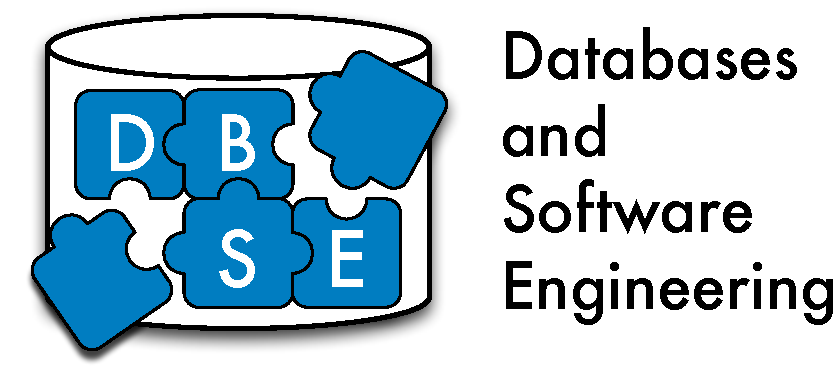
\includegraphics[scale=.45]{DBSE}}

\newcommand{\signatureplace}{Magdeburg}

\newcommand{\advisorone}{Prof. \ {Dr. rer. nat. habil. Gunter Saake}}
\newcommand{\departmentone}{\ifgerman{Institut für}{Institute for}Technical and Operational Information Systems}

\newcommand{\advisortwo}{}
\newcommand{\departmenttwo}{}
\newcommand{\setdate}{}
% Thesis kind
\ifgerman{\newcommand{\thesiskind}{Masterarbeit}}{\newcommand{\thesiskind}{Master's Thesis}}
%\ifgerman{\newcommand{\thesiskind}{Bachelorarbeit}}{\newcommand{\thesiskind}{Bachelor Thesis}}
%\newcommand{\thesiskind}{Diplomarbeit} %do not translate
%\ifgerman{\newcommand{\thesiskind}{Doktorarbeit}}{\newcommand{\thesiskind}{Dissertation}}

\ifgerman{
	\newcommand{\theforename}{\todo{Vorname}}
	\newcommand{\thesurname}{\todo{Nachname}}
	\newcommand{\thetitle}{\todo{Titel der Arbeit}}
	\newcommand{\thedate}{\todo{13. Monat 2014}}
}{
	\newcommand{\theforename}{Jay Dilipbhai}
	\newcommand{\thesurname}{Vala}
	\newcommand{\thetitle}{Classification of multilingual legal text Using deep learning: Evaluation of General-Purpose Resources for a Legal Domain-Specific Task}
	\newcommand{\thedate}{4. Monat 2019}
	
}
\newcommand{\theyear}{2019}
% date for signature in erklaerung.tex (declaration of originality)
\newcommand{\signaturedate}{4. Monat 2019}

%*********************************************************************%
% SETUP                                                               %
%*********************************************************************%

% meta informations of the document
\hypersetup{
 pdfauthor={\theforename\ \thesurname},
 pdftitle={\thetitle}
}

% open index file
\ifnotdraft{\makeindex}

%*********************************************************************%
% ACRONYMS                                                            %
%*********************************************************************%

% HOWTO: \gls{IDE} for singular or \glspl{IDE} for plural with 's
\makeglossaries
\newacronym{SVM}{SVM}{Support Vector Machines}
\newacronym{LSTM}{LSTM}{Long Short Term Memory}
\newacronym{BiLSTM}{BiLSTMs}{Bidirectional Long Short Term Memory}
\newacronym{TF-IDF}{TF-IDF}{Term Frequency Inverse Document Frequency}
\newacronym{AI}{AI}{Artificial Intelligence}
\newacronym{NLP}{NLP}{Natural Language Processing}
\newacronym{ANN}{ANN}{Artificial Neural Network}
\newacronym{RNN}{RNN}{Recurrent Neural Network}
\newacronym{CNN}{CNN}{Convolutional Neural Network}
\newacronym{TP}{TP}{True Positive}
\newacronym{TN}{TN}{True Negative}
\newacronym{FP}{FP}{False Positive}
\newacronym{FN}{FN}{False Negative}
%\glsaddall % use only if you have acronyms that occur only in graphics

%*********************************************************************%
% THE DOCUMENT                                                        %
%*********************************************************************%

\begin{document}

\ifgerman{
	\labelformat{lstlisting}{Quelltext~#1}
	\renewcommand{\lstlistingname}{Quelltext}
}{
	\labelformat{lstlisting}{Listing~#1}
}

% set the path where graphics are located
\graphicspath{{pics/}}

\ifnotdraft{
	\frontmatter
	\pagenumbering{roman}
	\newcommand{\theauthor}{\theforename\ \thesurname}
\newcommand{\theauthorr}{\thesurname,\ \theforename}
\begin{titlepage}
 \thispagestyle{empty}
 \begin{center}
  {\university}\\[0.4cm]
  {\school}\\[2.0cm]
   \hbox{}\hfill
    \begin{minipage}[t]{\textwidth}
      \begin{center}
        \logo
	  \end{center}
    \end{minipage} 
   \hfill\hbox{}
  \ \\[0.4cm]
  \ifdbse{
  {\large \thesiskind \\[1cm]}
  {\huge\bf \thetitle \\[1cm]}
  }
  {
  {\large \thesiskind \\[1.6cm]}
  {\huge\bf \thetitle \\[1.6cm]}
  }
  { \ifgerman{Autor:}{Author:}}\\[0.4cm]
  {\huge \theauthor}\\[0.8cm]
  {\large\thedate}\\[0.8cm]
  {\ifgerman{Betreuer:}{Advisors:}}\\[0.4cm] 
  {\large
\advisorone
  }\\[0.2cm]
  {
\departmentone
  }\\[0.8cm]
  {\large
\advisortwo\ 
  }\\[0.2cm]
  {
\departmenttwo\ 
  }
 \end{center}
\end{titlepage}

%%%%%%%%%%%%%%%%%%%%%%%%%%%%%%%%%%%%%%%%%%%%%%%%%%%%%%%%%%%%%%%%%%%%%%%%%%%%
%%% Titelrückseite: Bibliographische Angaben
%%%%%%%%%%%%%%%%%%%%%%%%%%%%%%%%%%%%%%%%%%%%%%%%%%%%%%%%%%%%%%%%%%%%%%%%%%%%

\thispagestyle{empty}
\vspace*{\fill}
\begin{minipage}{15.0cm}
\textbf{\theauthorr:}\\
\emph{\thetitle\\}
\thesiskind, \university, \theyear.
\end{minipage}
\newpage

	\ifgerman{\chapter*{Inhaltsangabe}}{\chapter*{Abstract}}
With the plethora of legal corpora available online, it can be overwhelming and hard to comprehend for a non-domain expert. \gls{AI} can be helpful in the organization and exploration of these document \cite{merkl1997exploration}.  Classifying these legal texts into higher level categories using machine learning and deep learning can not only help in the organization of these documents but can also help the non-domain user to navigate and find the relevant documents easily. The diversity, the advantages and the drawbacks of these algorithms makes choosing the algorithm a time-consuming and challenging process.

This thesis goes into investigating a few popular machine learning and deep learning algorithms with different configurations on EUR-Lex Summaries legal data for text classification. It also examines the feasibility of general-purpose resources used by deep learning algorithms for their performance on legal domain-specific data and the performance benefits of using multilingual data which is widely available for legal corpus. These experiments help us in exploring the viability of these algorithms in domain-specific settings and improve our decision-making process.  For the investigation, three different research questions are formulated, first comparing supervised machine learning algorithm  \gls{SVM} to deep learning algorithm \gls{BiLSTM}, second comparing the general-purpose word embeddings to the domain-specific word embeddings for training \gls{BiLSTM} and third comparing performance evaluation of multilingual data to monolingual ones in \gls{BiLSTM}.

Furthermore, with the limited labeled legal domain dataset, and class imbalance, several alternate training, and evaluation strategies were formulated. The training is done on sentences of the document with and without clustering, and the evaluation is done of sentences as well as on documents through the combination of predictions from the sentence. During the evaluation it is observed that adding more languages in case of \gls{BiLSTM} indeed increase the performance of the classifier.
































	\blankpage
    
    % The whole acknowledgement is meant to be written here, so great.
	\chapter*{Acknowledgements}
	 \begin{quote}
	    ``Life is like a box of chocolates. You never know what you’re gonna get" - Forrest Gump
	 \end{quote} 


    Last year in November, I embarked on this fascinating journey of undertaking my Master thesis unaware what lies ahead,  just like a box of chocolates. It gives me immense pleasure and a sense of satisfaction to finish this thesis. This thesis would not have been completed had there not been a few people to support and guide me all along.
    
    First and foremost, I want to thank my supervisor M.Sc. Sabine Wehnert, without whom this thesis would not have been possible in the first place. Her constant support, discussions, and assistance at every step were very helpful. I want to thank M.Sc. Marcus Thiel, for his assistance and suggestions on validating various concepts, and Stefan Langer for his support and ideas.
    
    I want to thank my Mom, Dad, Sister, and Brother for their moral and financial support. They stood by me in my thick and thin. I can not even begin to describe the gratitude and appreciation for their support.
    
    I want to thank my friends for listening to me, and at times tolerating me. They were like a family away from home. 
    
    Last but not least I would like to thank everyone who has supported me directly or indirectly throughout this thesis.


    
	\blankpage
}

%*********************************************************************%
% LISTINGS                                                            %
%*********************************************************************%

\ifnotdraft{
	{\parskip 0pt \pdfbookmark{\contentsname}{\contentsname}\chapterheadfont \tableofcontents} % toc bitte einzeilig
	\blankpage

	\ifgerman{
		\listoffigures
		\addcontentsline{toc}{chapter}{Abbildungsverzeichnis}

		\listoftables
		\addcontentsline{toc}{chapter}{Tabellenverzeichnis}

		\renewcommand{\lstlistlistingname}{Quelltextverzeichnis}
		\blankpage
		\lstlistoflistings
		\addcontentsline{toc}{chapter}{\lstlistlistingname}

		%\renewcommand*{\firstacronymfont}[1]{\emph{#1}}
		%\printglossary[type=acronym,title=List of Acronyms,toctitle=Abkürzungsverzeichnis]
	}{
		\listoffigures
		\addcontentsline{toc}{chapter}{List of Figures}

		\listoftables
		\addcontentsline{toc}{chapter}{List of Tables}

		%\renewcommand{\lstlistlistingname}{List of Code Listings}
		%\blankpage
		%\lstlistoflistings
		%\addcontentsline{toc}{chapter}{\lstlistlistingname}

		\renewcommand*{\firstacronymfont}[1]{\emph{#1}}
		\printglossary[type=acronym,title=List of Acronyms,toctitle=List of Acronyms]
	}
}

%*********************************************************************%
% CHAPTERS                                                            %
%*********************************************************************%

\mainmatter
\pagenumbering{arabic}

\ifgerman{\chapter{Einführung}}{\chapter{Introduction}}

%- Hintergrund
%- Motivation
%- Ziele
%- Aufgaben
%- Allgemeine Beschreibung des Projektes
%- Worum geht es in dieser Arbeit?
%- Wer hat die Arbeit veranlasst und wozu?
%- Wer soll von den Ergebnissen profitieren?
%- Welches Problem soll gelöst werden? Warum?
%- Unter welchen Umständen braucht man eine Verbesserung?
%- Was ist der Stand der Technik?
%- Welche noch offenen Probleme gibt es?
%- Worin unterscheidet sich mein Ansatz von den bisherigen?
%- Welche Ziele hat die Arbeit?
%- Wie will ich diese Ziele erreichen?
%- Was habe ich im Einzelnen vor?

% \hint{}

% \hint{\ldots\ to be continued \ldots}

\section{Introduction}
\glsresetall
There is an abundance of legal corpora available online. The publications office of the European Union (EU) offers different EU laws such as Treaties, Legal acts, Consolidated texts, International agreements, Preparatory documents and Summaries of EU Legislation. It also provides EU case laws, national laws, and national case laws. Other governments in the EU also publish legal text such as the \textit{gesetze-im-internet} website, the German Federal Ministry of Justice and Consumer Protection and the Federal Office of Justice offerings of every federal law of Germany, the \textit{Library of Congress} for the French law and many more.

Large legal text corpora can be overwhelming and hard to comprehend for non-domain experts, especially when jargon is used. Also, the complexity and the capricious nature of the legal texts is a challenge in itself. It can also be challenging for domain experts handling legal text written for different demographics, with different structure, and in different languages. Some of the most common problems with the legal texts are that it may be coming from different sources (different department of the government or from different governments altogether), it is difficult to know which laws overturn other laws, understanding different lexicon that changes with contexts, authority and over time \cite{boella2012nlp}. These barriers make it challenging to organize and aggregate these legal texts in a coherent manner. Traditional full-text search matches the exact text, and this helps in finding relevant information, but it is still challenging to discover all the relevant information such as in the cases where related words and synonyms are used for search \cite{landthaler2016extending}. To get around this, domain ontologies which map the relationships of synonyms, related words and antonyms are used; however, these are hard to create and difficult to maintain. 

The ongoing advancements in \gls{AI} and Machine Learning which is partly due to the availability of computing power can be promising in mitigating some of the difficulties with legal texts mentioned above. \gls{NLP} is a subset of \gls{AI} that focuses on systems that can learn and understand language. \gls{ANN} are a part of AI which was inspired by the biological neural network of human brain \cite{van2018artificial}. They are a framework comprising many different machine learning algorithms learning complex data. The application of \gls{ANN} is suitable for data that has noise which in case of legal text is having no sole representation of a law, that is the perception of law is in accordance with the requirements and needs. Secondly, there is a poor understanding intrinsic structure which means that there is no single entity which knows all the laws and lastly for the data having changing characteristics \cite{merkl1997exploration}. 

Various methods involving machine learning and \gls{AI} have been developed to solve some of the problems with legal texts described above. de Maat et. al (2010) \cite{de2010machine} have shown the effectiveness of using machine learning algorithms to classify legal text compared to a pattern-based classification task on unseen data. Mozina et. al (2005) \cite{movzina2005argument} showed that argumentation-based machine learning can be made using the justification of the case laws making it suitable for legal domain-specific tasks. Boella et. al (2011) \cite{boella2011using} have shown that sophisticated legal document management systems can be further improved using machine learning, the authors used classification algorithms to classify laws and integrate into an existing system. 



\section{Goals of this Thesis}
This thesis focuses on the classification tasks of legal text. There are various classification algorithms with their advantages and disadvantages. The goal of this thesis is to evaluate these algorithms in various configurations, 

Specifically, this thesis will investigate three questions,

\begin{itemize}
    \item 
        \begin{quote}
        Can deep neural network algorithms like \glsfirst{LSTM} networks perform comparatively to the thoroughly studied text classification algorithms like \glsfirst{SVM}?
        \end{quote}
        
        The \gls{SVM} has been thoroughly studied and applied in text classification \cite{Chau:2008:MLA:1322568.1322643, Fan:2006:ITM:1217741.1217764, Forman:2008:BFS:1458082.1458119,10.1007/BFb0026683,Sebastiani:2002:MLA:505282.505283,oro15675}. \glspl{SVM} have been shown to outperform many classification algorithms, but the sensitivity of the parameters to the classification task makes them difficult to use \cite{10.1007/978-0-387-34747-9_18}. Also the text representation technique used by the \gls{SVM} which is \gls{TF-IDF} does not capture the syntactics and semantics of the text \cite{Corr_a_J_nior_2017}. Many deep learning classification algorithms alleviate the problems that \glspl{SVM} posses, with text representation techniques such as word embeddings capturing the semantics and syntactics of the text to represent its context better.
        
        
    \item 
    \begin{quote}
        General-purpose resources such as pretrained word embeddings are getting better and are available from various sources and trained using different algorithms. As they are trained on large generic web scraped data, are they good enough for the legal domain-specific task?    
    \end{quote}
    Recently, various word embeddings such as BERT (Bidirectional Encoder Representations from Transformers) \cite{devlin2018bert}, Fasttext word vectors in 157 languages \cite{bojanowski2017enriching}, Flair \cite{akbik2018coling} and ELMo \cite{Peters:2018} were released. They, however, use general data scraped from websites like Wikipedia or freely available news and other corpora. These corpora do not cover the highly specialized and specific vocabulary used in the legal text; hence the effectiveness of these word embeddings for a legal domain-specific task has to be investigated.
    
    
    \item
    \begin{quote}
      Deep Neural Network algorithms like \gls{LSTM} can take advantage of multilingual data, as the text representation technique of word embeddings has been shown to work on multilingual data. Thus, the performance of \glspl{LSTM} needs to be investigated in case of monolingual and multilingual data to see if there is any advantage of using multilingual data.
    \end{quote}
     Conventionally, multilingual text classification is done by employing a language detector, which detects the language to be classified and then initiating a classifier that is trained on a specific language. This naive approach does not take advantage of the polylinguality of data for classification for a predefined category which may benefit from this data \cite{Wei:2014:EPD:2566999.2567111}. Recent techniques of learning bilingual word embeddings \cite{D13-1141,NIPS2014_5270} have shown to be improving, for this reason, the effect of multilingual embeddings is to be explored. 
\end{itemize}

\section{Structure of the Thesis}
The thesis is divided into seven chapters. \ref{ch:background} provides details of the various machine learning and deep learning methods, algorithms and information about document categorization. \ref{ch:concept} details the conceptual aspects for all the research questions and the techniques such as data cleaning, data collections that will be used to answer the research questions. \ref{ch:implementation} gives the detailed narrative of the tools used in implementing the concepts, the architecture and the hyperparameters of the algorithms provided in the \ref{ch:concept} and the specifics of how they are implemented. \ref{ch:evaluation} provides details of the evaluation approaches and the results of all the research questions.  \ref{ch:relatedwork} shows the similar work done on the legal dataset, and similar techniques used in training and evaluation of the algorithms. \ref{ch:conclusion} presents the conclusion of the thesis, discusses the limitations of some approaches and future works. 
\ifgerman{\chapter{Grundlagen}}{\chapter{Background}}
\label{ch:background}

This chapter covers the background  


\section{Document Categorization}
Due to the internet, we have access to an enormous amount of resources online. Governments, universities and other organizations constantly publish new documents which are hard to oversee. Organization and categorization of these documents is therefore important now more than ever. Due to organizations operating in different geographies, documents publish by them are available in multiple languages and are from different domains which makes it more difficult to categorize and retrieve them. For example, European Union publishes document in all the 24 official languages, big multinational companies like Volkswagen cars are present in 150 markets and are manufactured in more than 14 countries. Document categorization or Document classification is the analysis and assignment of documents into some predefined classes. Categorization is an important part of document retrieval as without categorization it is impossible to label the document and know when to present it to the user in response to the search query. Manually assigning these document (also refereed as indexing) is not feasible due to the continuous addition of new documents every day.

Classification of documents was first introduced by Luhn for creating abstracts in technical resources. Luhn proposed using statistical analysis of word occurrences in the abstract and title of the literature to assign it to a predefined category \cite{luhn1958automatic}. Many early adaptations of document categorization techniques relied upon carefully hand-crafted features \cite{Hayes:1990:CSC:645450.653070, Biebricher:1988:AIS:62437.62470}

\todo{write more}

\section{Machine Learning and Document Categorization}
In this section, we would discuss briefly about concepts of machine learning and its use in document and text categorization.  Machine learning is a field of Artificial Intelligence that provides the computers with the ability to learn and improve based on seen examples. Mitchell formally defines it as, ``\textit{A computer program is said to learn from experience $E$ with respect to some task $T$ and performance measure $P$, if its performance measure $P$ for the task $T$ improves with experience $E$}" \cite{Mitchell:1997:ML:541177}. Machine learning algorithms are divided into two types, \textit{supervised} and \textit{unsupervised} learning algorithms. Supervised learning algorithms learn from a given set of examples and try to predict on unseen target set. Unsupervised learning algorithms learn the relationships between elements of the given data. 

Text categorization or document categorization is a supervised learning problem. We have a set of training data which is labeled and is used to train the machine learning algorithm. This trained classifier is then used on the target or test set to predict the label.

\subsection{Supervised and Unsupervised Learning}
In supervised learning, a machine learning algorithm learns the mapping of a given set of examples to some specified, predefined categories. Formally, let $Z$ be the training set given by $\{(x_{1},y_{1}), (x_{2},y_{2}), (x_{3},y_{3}),...,(x_{n},y_{n})\}$ where $x_{i}$ are the input vectors to the algorithm and $y_{i}$ are the corresponding labels, then a supervised learning algorithm will try to learn the mapping function,

\begin{equation}
    f(X)  = Y
\end{equation}

The goal of this function is to approximate the mapping well enough that when a new data point $(x)$ is passed to the algorithm it can predict label $(y)$ from the data.

Contrary to the supervised way of learning, in unsupervised learning there are no corresponding labels, the algorithm has to model and learn the relationship of the underlying data. It is similar to learning without a teacher \cite{hinton1999unsupervised}.  
\todo{write more}

\todo{supervised(regression, classification), unsupervised}

\section{Multi-class vs Multi-label Classification}
Classification or categorization is the identification of an instance of data into a predefined category or class. Classification can be broadly divided into three types, \textit{Binary} \textit{Multi-class} and \textit{Multi-label} classification. Multi-class classification is the process of identifying an instance into one of many classes. In Binary classification the instances are classified into two classes hence the term \textit{binary}. There are various algorithms that solve the binary classification task. Several methods have been proposed to extend these binary classification problems into multi-class ones, as a multi-class problem can be seen as a set of several binary class problems \cite{aly2005survey}. Some of these extend naturally and some require special transformations to do so. Examples of this natural extension can Neural Networks as instead of having one a single neuron at the output as in binary classification, it has $N$ number of neurons for $N$ classes  \cite{bishop1995neural}. Other algorithms converts the multi-class problems into a set of binary classification problems for example Support Vector Machines \cite{cortes1995support}

In the Multi-label classification problem, instead of identifying an instance of data into a single category or class, it is identified into multiple classes. Multi-label classification is important in case of document classification as a document might contain aspects of different topics, so it is attributed into multiple classes. The most common approach to tackle the multi-label problem is to transform it into several binary or multi-class problems and then these predictions are transformed into multi-label predictions \cite{read2011classifier}.

\todo{write more about multi-label and multi-class with example}
\section{K-means Clustering}
It is often necessary to divide the data into groups in order to better understand it. Clustering is the process of grouping the data such that similar instances are grouped together (in same cluster) and dissimilar objects are grouped separately (in different clusters). Clustering is extensively used in data mining for statistical analysis in the earlier stages of exploratory analysis. The K-means clustering algorithm is an unsupervised machine learning algorithm. 

%It divides or partitions the data into $k$ different clusters \cite{macqueen1967some}. It does so by selecting $k$ randomly initialized cluster centers and refining them iteratively by first assigning each instance $x_{i}$ to the closest cluster center and then update each cluster center $C_{j}$ by mean of all the instances of that cluster. This converges when there is no further assignments of the instance or changes in the assignments of instances to the cluster.

The K-means algorithm separates data into $k$ clusters.  These clusters are such that they are as far away from each other as possible. Each cluster has a center data point (which is randomly initialized) called \textbf{centroid}, so the data point is assigned to a cluster if the point is close to this center.  K-means iteratively minimizes the distance between every data point and the center to find the optimal number of clusters.

Steps involved in K-means clustering is as follows,

\begin{enumerate}
    \item Initialize $k$ data points as centers (centroids) of the clusters.
    \item Calculate the distance between every point and the centroid, and based on this distance assign each point to a nearest cluster.
    \item The cluster centroids are updated by calculating the mean of all the points of that cluster.
    \item If the position of the centroids changes, then the process is repeated from step 2 until there is no change in the position of the centroid.
\end{enumerate}

The process stops when the average distance between the centroids and the distance between the points of a cluster is lowest. The minimal distance between the points of a cluster ensures that the cluster is compact with least variance between the points of a cluster.


\todo{example and equations}

\subsection{Pairwise constrained K-means } \label{constrainedKMeans}

Domain knowledge about the instances can be used to better assign the instances to clusters. It can be used to assess which instances should be or should not be grouped together \cite{wagstaff2001constrained}. There are two types of pairwise constraints.

\begin{itemize}
    \item \textbf{Must-link}: This constraint specifies that the two instances should be in same cluster.
    \item \textbf{Cannot-link}: This constraint specifies that the two instances should not be placed in same cluster.
\end{itemize}

This is a modified version of K-means clustering with the above mentioned constraints. The algorithm takes data $D$ and a set of \textit{must-link} constrains and a set of \textit{cannot links} constrains. As a result the data will be divided into $k$ groups satisfying all the constrains. When a data point is assigned to a cluster the algorithm ensures that it does not violate any of the specified constrains.

\todo{example}


\subsection{Choosing $k$}
To produce high quality clusters, the number of clusters ($k$) that the data needs to be divided into should be known. \textit{Silhouette Score} \cite{rousseeuw1987silhouettes} and \textit{Elbow Analysis} \cite{thorndike1953belongs,ketchen1996application}  are two methods to find out the number of clusters.

\todo{write more}
\subsubsection{Silhouette Score}
Silhouette score is a measure of the quality of a cluster. It determines how well an object fits the cluster assignment. Two things are necessary for the creation of silhouettes,first thing we need is the clusters and second we need the proximity between each of the cluster objects.

Let $s(x)$ be the silhouette score for element $x$ which is placed in cluster $A$ as shown in \ref{fig:sil_score}. We can calculate the dissimilarity $a(x)$ between elements $x$ of cluster $A$ and other elements of cluster $A$,
\begin{equation}\label{eq:sil_1}
    a(x) = \textit{average dissimilarity between x and other elements of cluster A}
\end{equation}
In \ref{fig:sil_score} $a(x)$ is represented by the average length of all the lines of cluster $A$. Now we calculate the dissimilarity of element $x$ with elements from cluster which is not $A$. For example, cluster $B$ which is different from $A$.

\begin{equation}\label{eq:sil_2}
    d(x,B) = \textit{average dissimilarity between x and other elements of cluster B}  
\end{equation} % In the pair wise clustering you forgot to mention anything in comment
In the \ref{fig:sil_score} $d(x,B)$ is represented by the average of lines stretching from element $x$ in the  cluster $A$ to all the elements in the cluster $B$. Once this is calculated for all the clusters, the minimum of these numbers is selected and denoted by 
\begin{equation}\label{eq:sil_3}
    b(x) = minimum(d(x, B))
\end{equation}

Here, for cluster $B$ we have the minimum of $b(x)$, so cluster $B$ is called the \textit{neighbour} of $x$, this is the second best option for $x$, if it cannot be accommodated in cluster $A$.

To calculate the silhouette score of $s(x)$, we use $a(x)$ and $b(x)$ obtained in \ref{eq:sil_1} and \ref{eq:sil_3}

\begin{equation}
    s(x) = \frac{b(x)-a(x)}{max\{a(x),b(x)\}}
\end{equation}


\begin{figure}[!ht]
    \centering
    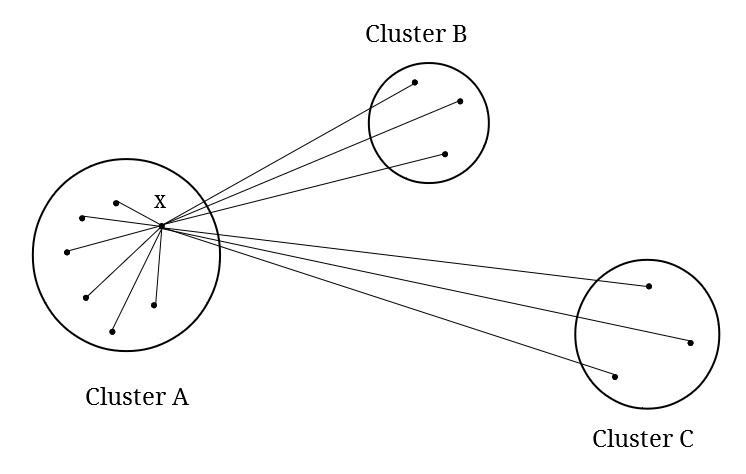
\includegraphics[width= 10cm, keepaspectratio]{pics/sil_score.jpg}
    \captionsetup{justification=centering,margin=2cm}
    \caption{Computation of silhouette score $s(x)$ with three clusters for point $x$ in cluster $A$.}
    \label{fig:sil_score}
\end{figure}


\subsubsection{Elbow Analysis}
Elbow analysis \cite{thorndike1953belongs,ketchen1996application} is another method of finding the number of clusters ($k$). The K-means algorithm works by finding the clusters which minimize the within cluster variance. The sum of squares of all the points in a cluster explains the variance within a cluster and hence it is used in elbow analysis to find the optimal number of clusters. 

Elbow analysis uses the within cluster sum of errors (WCSS). WCSS is calulated as the sum of distances of each point of a cluster and the centroid of that cluster. 

\todo{redraw the figure}
\begin{figure}[!ht]
    \centering
    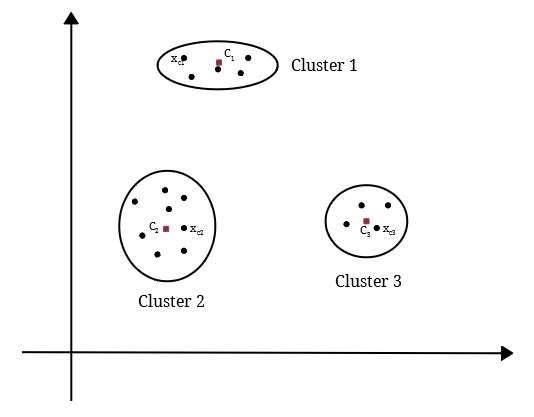
\includegraphics[width=8cm,keepaspectratio]{pics/Elbow.jpg}
     \captionsetup{justification=centering,margin=2cm}
    \caption{An illustration of clusters and centroids, with three clusters and their respective centroids $C_{1}$, $C_{2}$, $C_{3}$}
    \label{fig:elbow}
\end{figure}

For the clusters in the \ref{fig:elbow}, WCSS will be calculated as follows.
\begin{equation}
   WCSS = \sum_{i=1 }^{n}\sum_{k=1}^{n}distance(x_{i,j},C_{k})
\end{equation}

where:
\begin{align*}
      & x_{i,k}=\text{Data point $i$ in cluster $k$}\\
      & C_{k}=\text{Centroid for cluster $k$}\\
\end{align*}

This WCSS distances is plotted against the number of clusters which show an elbow shape; adding more clusters will decrease the information gain and will not model the data better.

\begin{figure}[!ht]
    \centering
    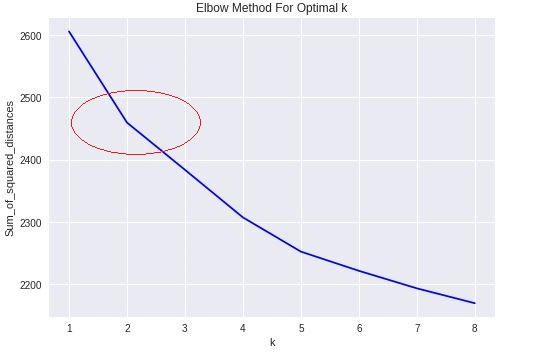
\includegraphics{pics/Elbow_example.jpg}
     \captionsetup{justification=centering,margin=2cm}
    \caption{Illustration of elbow at $k =2$ }
    \label{fig:elbow_at_2}
\end{figure}

In the \ref{fig:elbow_at_2} we can see the elbow shape at $k=2$ on the x axis. This suggest that we divide the data into two clusters.

\todo{why elbow is not trust worth and why it has to be used with silhouette scores.}

\clearpage
\section{Support Vector Machine}\label{sec:svm}
Text Categorization is an important technique for handling and organization of text corpora. The aim of categorization is the classification of text into some predefined categories. Support Vector Machines are based on \textit{Structural Risk Minimization},
which aims to find out a hypothesis $h$ for which we have the lowest \textit{true} error. The true error of $h$ is the probability that $h$ will make an error on the unseen and randomly selected data. Support Vector Machines are universal learners, also their ability to learn is independent of the dimensionality  of the input features. The dimensionality is high in case of text and also most text categorization problems are linearly separable \cite{joachims1998text}, which makes them suitable for text categorization.   

%\todo[inline]{About svm and how it works}
A Support Vector Machines is a supervised learning algorithm. It tries to find linear (in case of Linear SVM Kernel) boundaries in the given feature space. An SVM tries to maximize the distance between the two points of a decision surface \cite{manning2010introduction}.

\begin{figure}[!ht]
    \centering
    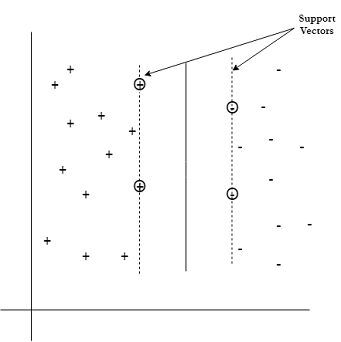
\includegraphics{pics/svm.png}
    \captionsetup{justification=centering,margin=2cm}
    \caption{Support Vector Machines}
    \label{fig:svm}
\end{figure}

 

% The following paragraph will be in the implementation chapter



\clearpage
\section{Deep Learning} \label{sec:DeepLearning}

The rise in digitization brought in the problem of creation of huge and diverse unstructured data. With the increase in computation power and the need to analyse the data to get better insight of it has given rise to deep learning. Deep learning is a sub category of artificial intelligence which is inspired by human brain and replicate the way a human learns. An Artificial Neural Network (ANN) mimics the human brain. Basic neural network will have an input layer, one output layer along with a hidden layer consisting of units that process given input into something that the output layer can use.   ANNs are incredible tools for recognizing patterns which are way too complex for programmers to extract and teach the machine to recognize.Neural Networks have been in to existence since last century, however it is during last decade they have become a major part of artificial intelligence due to the technique called backpropagation.

An artificial neuron is the building block of an ANN. Every input is multiplied with random weights so that the inputs are weighted.  These weighted inputs are then summed up with biases and passed through a transfer function and then the net input is passed through the activation function.

\begin{figure}[!ht]
    \centering
    \captionsetup{justification=centering,margin=2cm}
    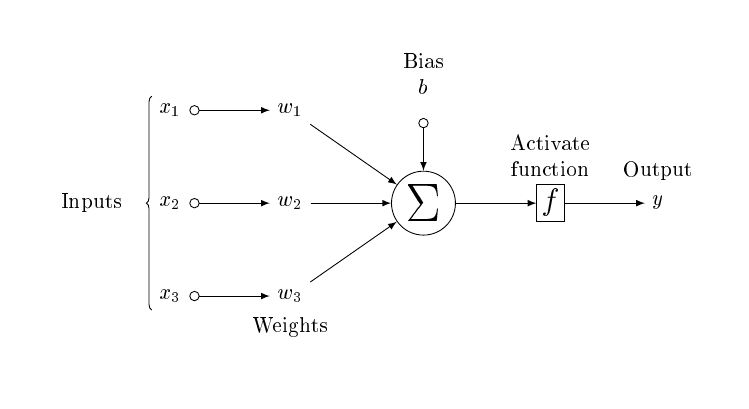
\includegraphics[width=12cm]{pics/ArtificialNeuronModel.png}
    \caption{An Artificial Neuron}
    \label{fig:neuron}
\end{figure}

The output of the neuron in the \ref{fig:neuron} would be as follows:

\begin{equation}
y=f(x_{1}w_{1}+x_{2}w_{2}+x_{3}w_{3}+b)
\label{eq:NNformula}
\end{equation}

Although the structure and computation of a single artificial neuron looks simple and easy, but its full potential and power of calculation is realized when they are interconnected and made into an artificial neural network. An artificial neural network comprises of an input layer, hidden layers and output layer as shown in \ref{fig:NN}.
\begin{figure}[!ht]
    \centering
    \captionsetup{justification=centering,margin=2cm}
    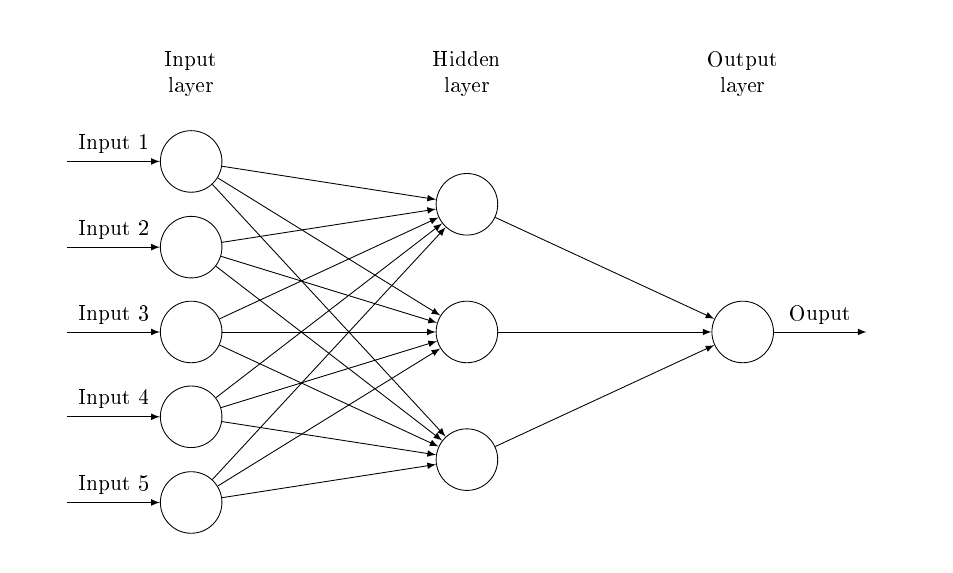
\includegraphics[width=10cm]{pics/neural_network.png}
    \caption{Artificial Neural Network}
    \label{fig:NN}
\end{figure}

A single neuron is not powerful enough to solve big and complex real world problems, but when they are put together in a specified topology or architecture they can be very handy in solving the same task a single neuron fails to do so. Advantage of artificial neural network is that these neurons can process data in distributed way, in parallel, non-linearly and locally \cite{andrej2011introduction}.
\\
\\
\\
\par
The ways in which these neurons are connected is what makes them so powerful. There are basically two main topologies in which these neurons are connected. 
\begin{figure}[!ht]%
\centering
\subfigure[Feed forward neural network]{%
\label{fig:FFRNfirst}%
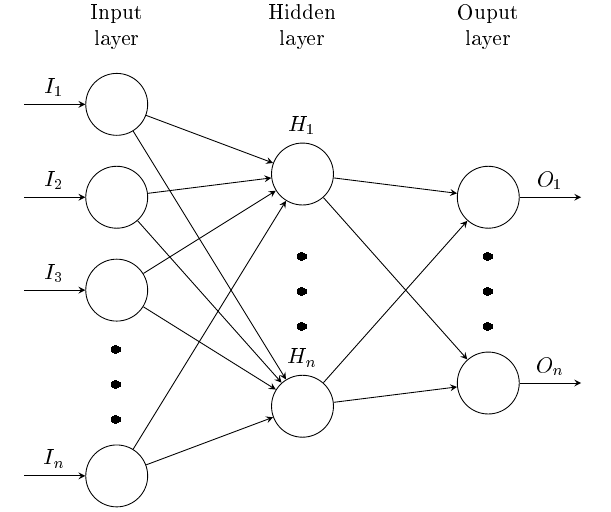
\includegraphics[height=4cm]{pics/nn2.png}}%
\qquad
\subfigure[Recurrent neural network]{%
\label{fig:FFRNsecond}%
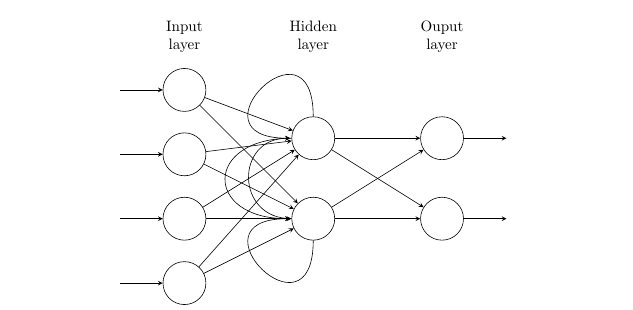
\includegraphics[height=4cm]{pics/rnn.png}}%
\caption{sample}
\label{fig:FFRN}
\end{figure}

As we can see from the \ref{fig:FFRNfirst} that in feed forward neural network the flow of information is only in one direction that is from inputs to the outputs wherein in the recurrent neural network the information flows in many possible directions as show in the  \ref{fig:FFRNsecond}

\subsection*{Activation functions}
Activation functions are important features of artificial neural networks. Activation functions is described as a function which converts the input into outputs. Consider the example of flow of current in an electric circuit as information flow in a neural network, switch in the circuit as activation function in neural network. Hence, an activation function is responsible for \textit{ON} and \textit{OFF} state of the circuit depending on the input. As the artificial neurons are inspired by the biological neuron, the activation function in biological from is either the neuron is firing or not.   

The activation function is a non linear transformation applied to the input. When the non linear transformation is not applied to the input, the output that we get would be a linear transformation, which is rather easy to solve but will not model many real world complex problems. A neural network without the activation is basically a linear regression model. The use of activation function is highly dependent on the problem at hand. Some of the most common activation functions are listed below.

\subsubsection*{Sigmoid activation function}
Sigmoid is one of the most common activation function used in neural networks. This function is widely used because its easy to calculate their derivatives, which makes weights calculation very easy in some cases. Sigmoid activation can suffer from the vanishing gradient problem.\cite{bengio1994learning}. Vanishing gradient occurs when layers of a neural network have gradients of $0$ because layers above them have saturated between -1 and 1. \cite{maas2013rectifier}


%equation of sigmoid
\begin{equation}
S(x) = \frac{1}{1+e^{-x}} \\
\label{eq:sig}
\end{equation}

\begin{figure}[!ht]
    \centering
    \captionsetup{justification=centering,margin=2cm}
    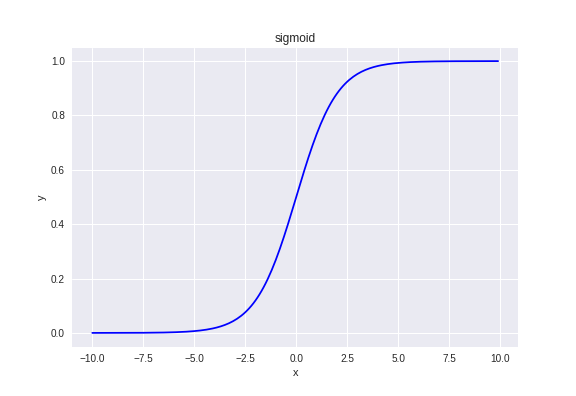
\includegraphics[width=9cm, height=9cm, keepaspectratio]{pics/sigmoid_10.png}
    \caption{Sigmoid activation function}
    \label{fig:sigmoidActivation}
\end{figure}

\subsubsection*{Rectified Linear Unit (ReLU) activation function}
The Rectified Linear Unit function is the most popular activation function from deep neural networks. The Rectified Linear Unit offers alternative nonlinearities compared to sigmoid functions, which mitigates the problem of sigmoids vanishing gradient, however during optimization procedure when these units are inactive the gardient is $0$ which leads to the problem of these units never getting activated as gradient based optimization will never adjust the weights of units which did not activate initially \cite{maas2013rectifier}\\
%equation of relu
\begin{equation}\label{eq:ReLU}
f(x) = \begin{Bmatrix}
0 & x < 0 \\ 
x & x \geq 0 
\end{Bmatrix}
\end{equation}
%graph of relu
\begin{figure}[h]
\centering
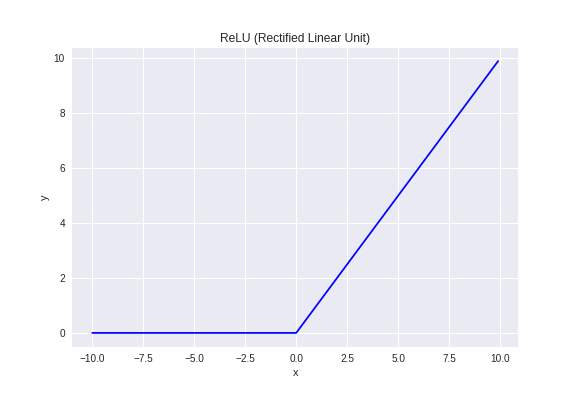
\includegraphics[width=9cm, height=9cm, keepaspectratio]{pics/ReLU_10.png}
\caption{Rectified Linear Unit Activation Function}
\label{fig:ReLU}
\end{figure} 

\subsubsection*{Hyperbolic Tangent}
This function is defined as ratio between the hyperbolic sine and hyperbolic cosine functions. Characteristics of this function is similar to sigmoid function. It outputs the values between -1 and 1 as it can be seen in the \ref{fig:tanh}

%eq 
\begin{equation}\label{eq:tanh}
f(x) = tanh(x)=\frac{2}{1+e^{-2x}} -1
\end{equation}
%fig
\begin{figure}[h]
\centering
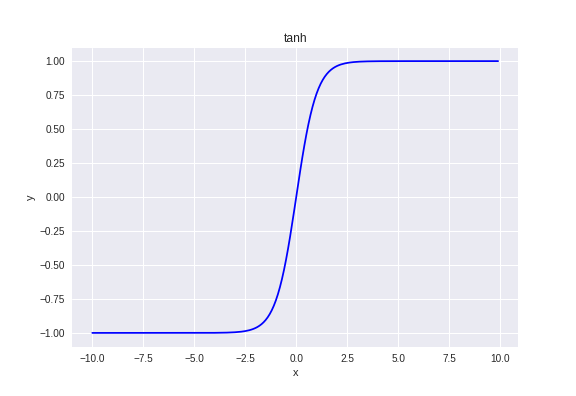
\includegraphics[width=9cm, height=9cm, keepaspectratio]{pics/tanh_10.png}
\caption{TanH Activation Function}
\label{fig:tanh}
\end{figure} 

\subsection*{Softmax activation function}
Softmax activation function is a generalization of the logistic function, in probability theory the output of the softmax function can be used to represent a categorical distribution, that is a probability distribution over \textit{X} possible outcomes. Hence, softmax activation function is used in various multi-class classification in artificial neural networks \cite{wu2016deep}.
%equation forsoftmax
\begin{equation}\label{eq:softmax}
f(x_{i}) =\frac{e^{x_{i}}}{\sum_{N=1}^{J} e^{x_{i}} }     
\end{equation}

Where:
\begin{align*}
    f(x_{i}) &= \text{Probability of $i_{th}$ class}\\
    x_{i} &= \text{$i_{th}$ dimension output}\\
    N &= \text{Total number of classes}\\
\end{align*}

\subsection{Backpropagation}\label{backprop}
\todo{check backprop example in appendix. There is mistak in calculation of backward pass}
Backpropagation is shorthand for ``backward propagation of errors". In feed forward neural network when information flows from input layer to the each hidden layer to produce the output which is refereed to as \textbf{forward propagation} or \textbf{forward pass}. This forward pass continues to produce a scalar cost that is simply the difference between target (what the network should have produced, true target) and output (what network produced). The \textbf{backpropagation} or \textbf{backward propagation} algorithm allows this cost to flow backwards in the network to compute the new weights of the network \cite{goodfellow2016deep}. It is the learning procedure which adjust the weights of the connections in a network in order to minimize the difference between input vector and the desired output vector \cite{rumelhart1988learning}.

Consider a simple neural network with one input layer with 3 inputs namely $x_{1}$, $x_{2}$ and $x_{3}$, one hidden layer consisting of 2 neurons $h_{1}$ and $h_{2}$, and one output neuron, $o_{1}$. The activation function is a sigmoid activation and the cost function is simple Euclidean distance. 

\begin{figure}[!ht]
    \centering
    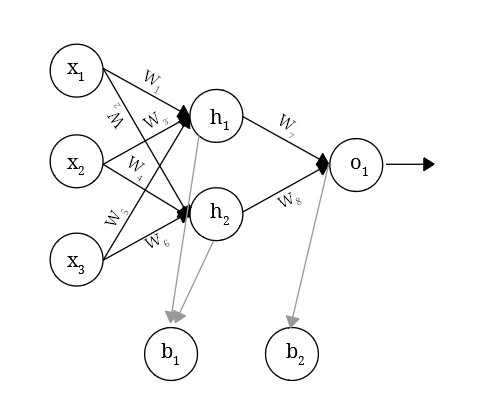
\includegraphics[width=9cm, height=6cm, keepaspectratio]{pics/backprop1.jpg}
    \caption{Single hidden layer neural network with one output}
    \label{fig:backPropExample}
\end{figure}

\subsection*{Forward pass}
In the forward pass the network will calculate the \textit{net} output of the hidden neurons, the apply the activation function to calculate the output of the hidden neurons and continue the process for the output layer neurons in the following way,
\begin{align}
    net_{h_{1}} &= (x_{1}w_{1}+x_{2}w_{3}+x_{3}w_{5}+b_{1})\\
    net_{h_{2}} &= (x_{1}w_{2}+x_{2}w_{4}+x_{3}w_{6}+b_{2})
\end{align}

Applying the activation function (sigmoid activation) to the \textit{net} output of the neurons of the hidden layers,

\begin{align}
    out_{h_{1}} &= \sigma (net_{h_{1}})\\
    out_{h_{1}} &= \frac{1}{1+e^{-net_{h_{1}}}}\\
    out_{h_{2}} &= \frac{1}{1+e^{-net_{h_{2}}}}
\end{align}
Then the \textit{net} output of the output layer is calculated by,
\begin{align}
    net_{o_{1}} &= (h_{1}w_{7}+h_{2}w_{8}+b)
\end{align}

Applying the activation function to the \textit{net} output to calculate the output of the output neuron $o_{1}$
\begin{align}
    out_{o_{1}} = \frac{1}{1+e^{-net_{o_{1}}}}
\end{align}

After the output at the output layer is obtained, the network will calculate the error or the cost function,

\begin{align}
    E_{\text(target, output)} &= \sum\frac{1}{2}(target-output)^2 \label{eq:backpropSUM} \\
    E_{total} &= E_{o_{1}} \\
    E_{total} &= \frac{1}{2}(target_{o_{1}}-out_{o_{1}})  
\end{align}

The error is calculated and this error is then used in the backward pass to calculate the new weights to be updated in order to minimize the error (Summation $\sum$ in the \ref{eq:backpropSUM} indicates that error will be calculated for each output neuron and then summed up).

\subsection*{Backward Pass}
In order to update the weights of the network, the effect to error on those weights is to be calculated, that is $\frac{\partial E}{\partial w}$, which is the rate of change of error function with respect to the weights also referred to as \textit{gradient} with respect to $w$. This is calculated by chain rule of calculus which is used to calculate the derivative of an unknown function by calculating the derivative of known functions.

The derivative of $\frac{\partial E_{total}}{\partial w_{7}}$ using chain rule is as follows,

\begin{align}
    \frac{\partial E_{total}}{\partial w_{7}} = \frac{\partial E_{total}}{\partial out_{o1}} * \frac{\partial out_{o1}}{\partial net_{o1}} * \frac{\partial net_{o1}}{\partial w_{7}} \label{eq:backPass}
\end{align}
Calculating each term individually,
\begin{align}
    \frac{\partial E_{total} }{\partial out_{o_{1}}} &= \text{change in total loss w.r.t output of $o_{1}$}
\end{align}
From , we can write,
\begin{align}
    E_{total} &= \frac{1}{2}(target_{o_{1}} - out_{o_{1}})^{2}
\end{align}

Taking the partial derivative of $E_{total}$ with respect to $out_{h_{1}}$, the part $\frac{1}{2}(target_{o_{2}} - out_{o{1}})^{2}$ becomes 0 because $out_{h_{1}}$ does not effect it and hence it is a constant.
\begin{align}
    \frac{\partial E_{total}}{\partial out_{o_{1}}} &= 2 * \frac{1}{2}(target_{o_{1}} - out_{o_{1}})^{2 - 1} \
\end{align}
Now for the second term in the equation \ref{eq:backPass}, we find out the rate of change of $out_{o_{1}}$ w.r.t $net_{o_{1}}$, hence we need to calculate the partial derivative of the sigmoid function. 
\begin{align}
    out_{o_{1}} &= \frac{1}{1-e^{net_{o_{1}}}}\\
    \frac{\partial out_{o_{1}}}{\partial net_{o_{1}}} &=  out_{o_{1}}*(1-out_{o_{1}}) \\
\end{align}
Finally, how much the $net_{o_{1}}$ changes w.r.t $w_{7}$,
\begin{align}
    net_{o_{1}} &= w_{7} * out_{h_{1}} + W_{8} * out_{h_{2}} + b_{2}   \\
    \frac{\partial net_{o_{1}}}{\partial w_{7}} &=  1 * out_{h_{1}} * w_{7}^{(1 - 1)} + 0 + 0
\end{align}

Calculating the new weight value $w_{7}$ using all the values from \ref{eq:backPass}, 

\begin{align}
    w_{7_{new}} &= w_{7} -\text{learning rate} * \frac{\partial E_{total}}{\partial w_{7}} \\ 
\end{align}

\subsection{Backpropagation Through Time}
The Backpropagation through Time (BPTT) is an extension of Backpropagation which is based on transforming a feedback network to a feedforward network by unfolding it over time \cite{ahmad2004recurrent}. Therefore, when a network processes a sequence which is $t$ times long, then $t$ copies of the network are created and the feedback connections are modified to be feedforward connections from one copy to another. This method is similar to training a large feed forward neural network with weights being modified and treated as shared weights.

\section{Text Representation}\label{backgroundTextRepresentation}

All text based computer systems requires some representation of textual data depending on the type of problem at hand. Unlike other data formats, textual data is semi structured or even unstructured. The representation of text in such system is done by transforming text into numerical form.  Detailed below are two of the most popular text representation techniques, TF-IDF and Word Embeddings.  

\subsection{Term Frequency - Document Inverse Frequency}
TF-IDF is the most common weighting method for describing textual data. Machine learning techniques such as Support Vector Machines and K Nearest Neighbours make use of this weighting scheme for text categorization. This technique works by first calculating \textit{Term Frequency} which is how often a word appears in a particular document and \textit{Inverse Document Frequency} which measure how infrequent a term is in the corpus \cite{soucy2005beyond}.

\textit{Term Frequency} is calculated as follows,

\begin{equation}\label{tf}
tf_{i,j} = \frac{n_{i,j}}{\sum_{k}n_{i,j}}
\end{equation}
where:
\begin{align*}
      & i=\text{word in the document}\\
      & j=\text{document from corpus}\\
      & k=\text{total documents in the corpus}      \\
      & n_{i,j}=\text{frequency of word $i$ in document $j$}      
\end{align*}                

Inverse Document Frequency (IDF) is a measure of importance of a word. In case of \textit{Term Frequency} all the words are considered equally important but in case of Inverse Document Frequency not all words are considered equally. While $IDF$ measures the importance of words in the corpus, some words which are referred to as \textit{stop words} such as \textit{is, of, are, the} which appear quite often in the document are of very little importance. Hence IDF will weigh less the frequently appearing words in the corpus compared to rarely appearing words. \cite{robertson2004understanding}. 

\begin{equation}\label{idf}
idf_{w} = \log\frac{N}{n_{i}}
\end{equation}
where:
\begin{align*}
      & N=\text{number of documents in corpus}\\
      & n_{i}=\text{number of documents with term $i$ in it}\\
\end{align*}     

From equation \ref{tf} and \ref{idf}, $TF-IDF$ score is computed as,

\begin{equation}\label{tf-idf}
w_{i,j} = tf_{i,j} \times \log\frac{N}{n_{i}}
\end{equation}
where:
\begin{align*}
      & tf_{i,j}=\text{number of times $i$ appears in $j$}\\
      & N=\text{number of documents in corpus}\\
      & n_{i}=\text{number of documents with term $i$ in it.}\\
\end{align*}

\subsection{Word Embeddings}
Conventionally, text representation in natural language processing involves techniques like \textit{bag-of-words} model in which a text is represented by the bag (words in the text), \textit{skip-gram} model which is generalization of \textit{n-grams} models where the words do not need to be successive for the text in consideration but can be skipped, hence named \textit{skip-gram} \cite{guthrie2006closer} and  \textit{tf-idf}. These techniques are a simple representation of various features. However, in the bag-of-words approach, grammar and word order are not considered. And in tf-idf only the importance of words is considered, \ref{sec:svm}. Hence, these techniques do not capture the semantics of the text. \cite{maas2011learning}.

Due to the above mentioned limitations, word embeddings were introduced. Word embeddings are a vector representation of the meaning of words in the corpus. This means that words are placed in a high-dimensional vector space where words with the similar meaning are placed close to each other. Neural network-based word vector models are usually trained using stochastic gradient descent where the gradient is obtained by backpropagation \cite{le2014distributed}.

To better understand how word vectors are employed, we consider an example of reviews of cars from 0 to 5 in various categories, where 0 is worst and 5 is best category. Lets say a car ``Volkswagen beetle" scores 3 on comfort (one of the evaluation criteria). Representing it on a scale and converting it from range 0 to 5 to 1 to -1.

\begin{figure}[!ht]
    \centering
    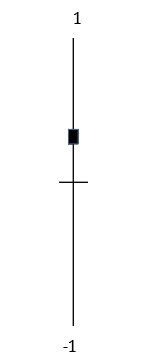
\includegraphics[width=2cm]{pics/wordVec.jpg}
    \captionsetup{justification=centering,margin=2cm}
    \caption{Comfort of ``Volkswagen beetle" on scale of 0-5, rescaled to range -1 to 1}
    \label{fig:volkswagan_example}
\end{figure}

Now this does not consider all the aspect of this approach. So, consider another evaluation criterion leg room (amount of space for your legs). Beetle has scored 4 in the leg room category. hence we represent it on a scale of -1 to 1 and add another dimension which represents the leg room category. 

\begin{figure}
    \centering
    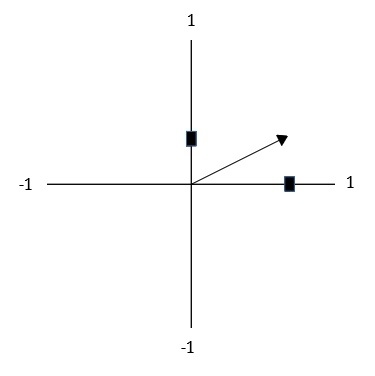
\includegraphics[width=5cm]{pics/wordVec_2.jpg}
    \captionsetup{justification=centering,margin=2cm}
    \caption{Comfort represented on x-axis and leg room on y-axis}
    \label{fig:volkswagan_example_2}
\end{figure}

Adding a few other cars we have a vector representation of those cars in a multi dimensional space (represented here in two dimensional space) \ref{fig:wordVecManyCars}


\begin{figure}[!ht]
    \centering
    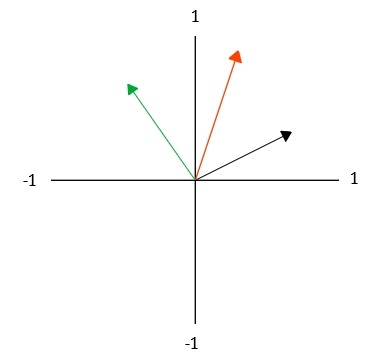
\includegraphics[width=5cm]{pics/wordVec_2_manycars.jpg}
    \captionsetup{justification=centering,margin=2cm}
    \caption{Vector representation of car features in a two dimensional space, black represents Volkswagen, red represents Mercedes and green represents Audi}
    \label{fig:wordVecManyCars}
\end{figure}


Using vectors, we can easily find the similarity between two cars using \textit{cosine similarity}.

\begin{table}[!ht]
\centering
\begin{tabular}{cc}
\hline
\textbf{Cars} & \textbf{Vectors} \\ \hline
Volkswagen    & 0.2, 0.4         \\ \hline
Mercedes      & 0.1, 0.6         \\ \hline
Audi          & -0.3, 0.5        \\ \hline
\end{tabular}
\caption{Vectors of cars}
\captionsetup{justification=centering,margin=2cm}
\label{my-label}
\end{table}

\begin{equation}
        \text{cosine-similarity (Volkswagen, Mercedes)} = 0.955 
\end{equation}
\begin{equation}
    \text{cosine-similarity (Volkswagen, Audi)} = 0.536
\end{equation}
\begin{equation}
    \text{cosine-similarity (Mercedes, Audi)} = 0.761
\end{equation}

Adding more dimensions captures more information and hence increases the quality of the results. These vectors represent the cars with numbers which is necessary for machines to understand and also we can calculate similarities between these vectors. 

One popular algorithm is \textbf{Word2Vec} \cite{mikolov2013efficient}, in this implementation word embeddings are trained using two models, \textit{continuous bag-of-words} model and \textit{continuous skip-gram model}. In continuous bag-of-words, the projection of words into the vector space is not influenced by the order of words and words from the future are also used in this model. In the Continuous Skip-gram model, instead of predicting next word based on the context, it tries to maximize the classification of next word based on other word in the fixed window size sentence.

Consider the following sentence to understand how the aforementioned methods works,

\begin{quote}
    \textit{I am the master of my fate, I am the captain of my soul} - Invictus, William Ernest Henley.
\end{quote}

\subsubsection*{Continuous Bag-of-words Model}
This model works by looking at words not only from a few words in the past but also a few words from the future to predict the target word. 

\begin{figure}[!ht]
    \centering
    
\includegraphics[width=12cm]{pics/bag-of-wordWord2Vec.jpg}
    \caption{Continuous bag-of-words model data set creation}
    \label{fig:word2VecBagOfWords}
\end{figure}

The target word is \textit{``fate"} and we want to predict it so we take a sliding window over the sentence as shown in \ref{fig:word2VecBagOfWords}. 

\begin{table}[!ht]
\centering
\begin{tabular}{ccccc}
\hline
\multicolumn{1}{l}{\textbf{Input 1}} & \multicolumn{1}{l}{\textbf{Input 2}} & \textbf{Input 3} & \multicolumn{1}{l}{\textbf{Input 4}} & \textbf{Output} \\ \hline
i & am & master & of & the \\ \hline
am & the & of & my & master \\ \hline
the & master & my & fate & of \\ \hline
master & of & fate & i & my \\ \hline
of & my & i & am & fate \\ \hline
\end{tabular}
\caption{Dataset for training continuous bag-of-words model}
\label{datasetBagOfWords}
\end{table}

This process will continue for the whole sentence in this case and whole corpus in case we have a big dataset. This dataset will then be feed into neural network for it to learn. 

\subsubsection*{Continuous Skip-gram Model}
This model tries to predict the neighbouring words based on the current word. So the training process for the above mentioned sentence is as follows.

We can take a sliding window over the sentence and construct a dataset for training the skip-gram model, 
\begin{figure}[!ht]
    \centering
    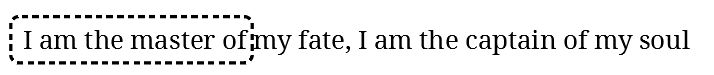
\includegraphics[width=12cm]{pics/skipgramWord2vec.jpg}
    \caption{Continuous skip-gram model dataset creation}
    \label{fig:skipgramWord2vec}
\end{figure}

We take the word \textit{``the"} and then start building the dataset as the word \textit{``the"} as input and the two left neighboring words \textit{``i"} and \textit{``am""} and the two right neighboring words \textit{``master"} and \textit{``of"} as shown in the \ref{fig:skipgramWord2vec}

\begin{table}[!ht]
\centering
\begin{tabular}{cc}
\hline
\textbf{Input} & \textbf{Output} \\ \hline
the            & i               \\ \hline
the            & am              \\ \hline
the            & master          \\ \hline
the            & of              \\ \hline
\end{tabular}
\caption{Dataset for training continuous skip-gram model}
\label{word2vec-skipgram-dataset}
\end{table}

This process will continue for the whole sentence until each and every word of the sentence is in the training dataset against its neighboring words. This dataset is then feed to the untrained neural network to predict the output.  

After the network converges, words with similar meaning are placed together in the embedding space. For example words like "powerful" and "strong" are placed close to each other in the vector space. \todo{Need to work on this, doesn't look good}


\todo{This following paragraph goes into implementation}

The model used in creation of the word vectors is a neural network, and neural networks are data hungry as it requires a lot of data to train them properly. As a result, another domain specific dataset is used in this experiment because dataset used for classification is small. Hence, the whole EUR-Lex dataset was used as it contains 19,348 documents mostly consisting regulations, decisions and directives of European Union \cite{jf:SemanticLaw}.

\subsection{Cross Lingual Word Embedding}\label{backgroundCrosslingual}

Word vectors for different languages are in different vector spaces, hence it can not be combined together, but the classification task involves classifying text from two languages, \textbf{English} and \textbf{German}. Hence, for classifying both languages within a single model is necessary. This not only mitigates the error caused by a language detector in multilingual systems, where a language detector first detects the language and then the respective classifier is invoked. In that affair, error propagates downwards and amplifies. And using multiple languages also increase the amount of data for training if multilingual parallel corpora is available where corpus of single language is low. 

To achieve this Duong et. al \cite{duong-EtAl:2016:EMNLP}, proposed using bilingual dictionaries and monolingual data. The model uses an extension of contextual bag-of-word(CBOW) model \cite{mikolov2013efficient}. This method has benefits as often there no parallel data when working on a domain specific problems, also it is comparatively easy to obtain or create bilingual domain specific dictionaries.

Facebook's MUSE Python library \cite{conneau2017word} aligns word vectors from multiple languages to a single vector space, the author claims that these embeddings state-of-art multilingual word embeddings, they have used Facebook's Fasttext \cite{bojanowski2017enriching} monolingual word embeddings and aligned them in common vector space. They use two sets word embeddings that are trained on monolingual data, and learns the mapping between these two embedding in a common vector space. It exploits the similarities of monolingual embedding space \cite{mikolov2013exploiting} to learn mapping between the two embeddings.

\subsection{Long Short Term Memory}
Neural networks have shown remarkable capabilities in processing and modeling natural language. Recurrent Neural Networks (RNN) and Convolutional Neural Networks (CNN) are common architectures for handling natural language. Long Short Term Memory (LSTM)\cite{hochreiter1997long} is a variant of RNNs, unlike other feed forward neural networks these networks have recurrent connections in them which allow information to persist.

\begin{figure}[!ht]
    \centering
    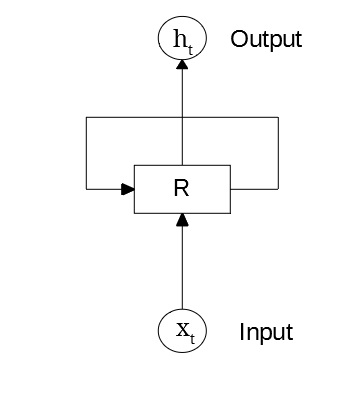
\includegraphics[width=4cm,height=6cm,keepaspectratio]{pics/rnn_cell.jpg}
    \captionsetup{justification=centering,margin=2cm}
    \caption{Single RNN Cell}
    \label{fig:rnn_single_cell}
\end{figure}

The \ref{fig:rnn_single_cell} shows a single RNN cell having a recurrent connection. This recurrent connection allows it to retain the previous state and make use of the context of the previous state \cite{graves2009novel}. Due to this property RNNs are very effective in processing text. 

RNNs are effective but suffer from the problem that the capacity of them to retain the previous states is fairly limited. The problem is that the input influences either diminishes the output or increases it exponentially. This is referred to as the problem of \textit{vanishing gradients}\cite{hochreiter2001gradient}. This problem makes it hard for RNNs to make use of more than a few previous states. LSTMs are a special kind of RNNs which address the problem of vanishing gradients. They contains recurrently connected sub-networks called \textit{memory blocks} and each of these blocks contains three gates; input gate, forget gate and output gate. These gates allows an LSTM to store information for a longer period of time. If the input gate is shut, that is if it has no activation (or close to 0), the activation of a block will not be overwritten for the next incoming inputs. Also, the block activation is only available to the network when the output gate is open. The forget gate switches on and off the recurrent connections.

\begin{figure}[!htbp]
    \centering
    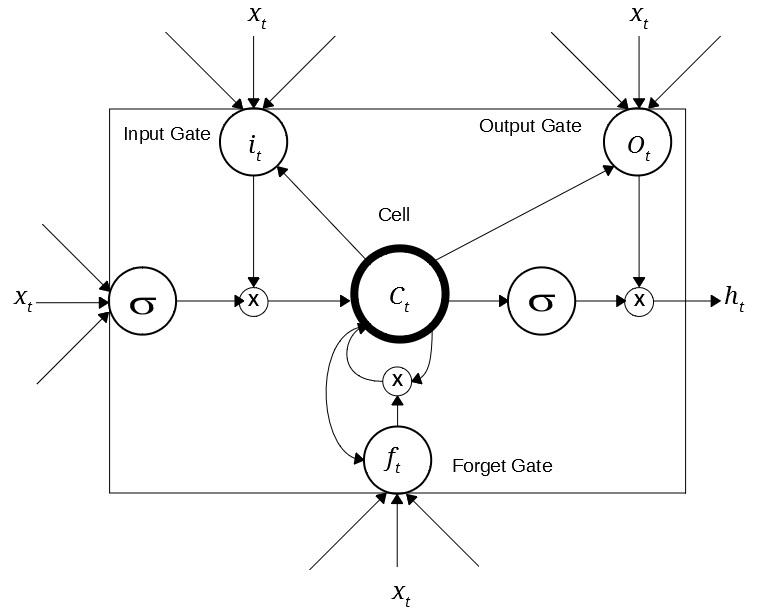
\includegraphics[width=10cm]{pics/lstm.jpg}
    \captionsetup{justification=centering,margin=2cm}
    \caption{LSTM block with a single cell. The cell has recurrent connections with a forget gate. The three gates collect inputs from rest of the network. }
    \label{fig:LSTM_BLOCK}
\end{figure}


Let $X$ $=$ ${x_{1}, x_{2},....,x_{n}}$ be the input sequence and $Y$ $=$ ${y_{1}, y_{2},....,y_{n}}$ be the output sequence. An LSTM network learns the mapping of input sequence to the output sequence using the following equations one by one from time $t$ $=$ 1 to $n$. Hence, the equation for the respective gates and the cell states are as follows:

\begin{equation} \label{eq:lstm_input_gate}
    i_{t} =\sigma(w_{i}[h_{t-1},x_{t}]+b_{i})
\end{equation}
\begin{equation}\label{eq:lstm_forget_gate}
    f_{t} =\sigma(w_{f}[h_{t-1},x_{t}]+b_{f})
\end{equation}
\begin{equation}\label{eq:lstm_output_gate}
    o_{t} = \sigma(w_{o}[h_{t-1},x_{t}]+b_{o})
\end{equation}

where:
\begin{align*}
      & i_{t}=\text{input gate}\\
      & f_{t}=\text{forget gate}\\
      & o_{t}=\text{output gate}\\
      & \sigma=\text{sigmoid function}\\
      & W_{i}=\text{Weight matrix of input gate}\\
      & W_{f}=\text{Weight matrix of forget gate}\\
      & W_{o}=\text{Weight matrix of output gate}\\
      & h_{t-1}=\text{output from previous block at time $t-1$}      \\
      & b_{i}=\text{bias for input gate}    \\
      & b_{i}=\text{bias for forget gate}    \\
      & b_{i}=\text{bias for output gate}\\
\end{align*}

The \ref{eq:lstm_input_gate} is for the input gate which allows whatever new information is to be stored in the cell state. \ref{eq:lstm_forget_gate} is for the forget gate which is responsible for discarding information that is not useful anymore from the cell state. \ref{eq:lstm_output_gate} is for the output gate which is responsible for the activation of the whole LSTM block at time $t$ 


\begin{equation}\label{eq:lstm_newCellState}
    \Tilde{c}_{t} =\tanh(w_{c}[h_{t-1},x_{t}]+b_{c})
\end{equation}
\begin{equation} \label{eq:lstm_CurrentCellState}
    c_{t} = f_{t} \odot c_{t-1} + i_{t} \odot \Tilde{c}
\end{equation}
\begin{equation}\label{eq:lstm_output}
    h_{t} = o_{t} \odot \tanh(c_{t})
\end{equation}
where:
\begin{align*}
      & \Tilde{c_{t}}=\text{new contender for cell state at $t$}\\
      & c_{t}=\text{current cell state at $t$}\\
      & \odot=\text{element wise product}
\end{align*}


% Yes I too thought so but I saw it is being done already
At any given time step, the current cell state knows what is to be forgotten, that is $f_{t}\odot c_{t-1}$ from \ref{eq:lstm_CurrentCellState} and which new cell state to be established from the current time step, that is $i_{t}\odot \Tilde{c}$ form \ref{eq:lstm_CurrentCellState}. This is then passed through a $\tanh$ function to filter out which of the two should be forgotten and which should be the output at the current time step. The output $h_{t}$ can then be passed through a softmax function to get the prediction probabilities for the current block.




\section{Bidirectional LSTM}
Bidirectional LSTMs are  able to access the context of a given sequence in both direction(forward and backward) \cite{schuster1997bidirectional}. In \ref{fig:BiLSTM} we can see that Bidirectional LSTM contains two layers out of which one processes the sequence in forward direction and one processes the sequence in backward direction. The output layer is connected to both layers which enables it to process both forward or future context and backward or past context. Bidirectional LSTMs have show to preformed better then standard LSTMs and RNNs in sequence learning data \cite{baldi2000bidirectional} \cite{fukada1999phoneme}.

\begin{figure}[!ht]
    \centering
    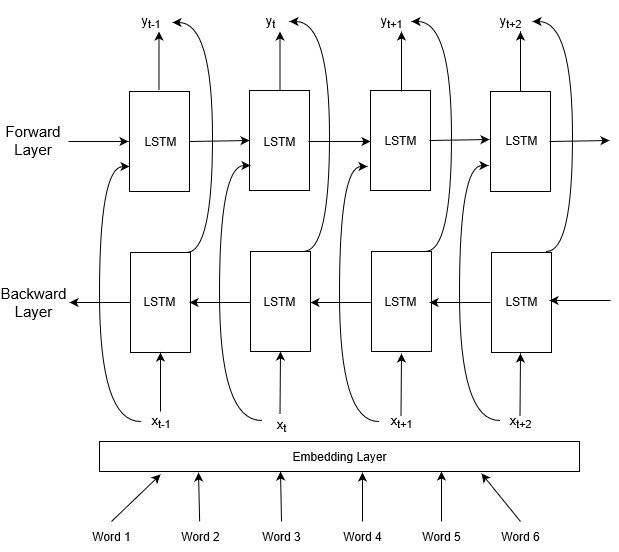
\includegraphics[width=12cm,height=8cm,keepaspectratio]{pics/BiLSTM.jpg}
    \captionsetup{justification=centering,margin=2cm}
    \caption{Bidirectional LSTM }
    \label{fig:BiLSTM}
\end{figure}

From \ref{fig:BiLSTM}, it can be seen that there is no connection between the forward passing layer and backward passing layer, hence outputs from forward pass is not connected to the input of backward class and vice versa, so training a Bidirectional LSTM is same as unidirectional LSTM for the most part.

\section{Data Distribution}
There are many inconsistencies when it comes to the number of documents in the classes. In the class \textit{justice freedom and security} there are \textit{320} documents for English corpus and \textit{314} documents for German corpus. These irregularities are of less importance when it comes to learning them separately, but becomes important when both languages are to be learned together. Information can leak from training to testing set leading to unrealistic results if these inconsistencies are not dealt with earlier. 

\begin{figure}[!ht]
\begin{center}
\makebox[2pt]{
\begin{tikzpicture}
  \centering
  \begin{axis}[
        ybar, axis on top,
        title={},
        height=7cm, width=15cm,
        bar width=0.2cm,
        ymajorgrids, tick align=inside,
        enlarge y limits={value=.1,upper},
        ymin=0, ymax=600,
        axis x line*=bottom,
        axis y line*=left,
        y axis line style={opacity=0},
        tickwidth=0pt,
        ytick style={draw=none},
        enlarge x limits=true,
        legend style={
            at={(1,1)},
            anchor=north east,
            legend columns=-1,
            /tikz/every even column/.append style={column sep=0.1cm}
        },
        ylabel={number of documents},
        symbolic x coords={
        agriculture,
        audiovisual  and  media,
        budget,
        competition,
        consumers,
        culture,
        customs,
        development,
        economic  and  monetary  affairs,
        education  training  youth,
        employment  and  social  policy,
        energy,
        enlargement,
        enterprise,
        environment,
        external  relations,
        external  trade,
        fight  against  fraud,
        food  safety,
        foreign  and  security  policy,
        human  rights,
        humanitarian  aid,
        information  society,
        institutional  affairs,
        internal  market,
        justice  freedom  security,
        maritime  affairs  and  fisheries,
        public  health,
        regional  policy,
        research  innovation,
        taxation,
        transport
        },
       xtick=data,
       x tick label style={rotate=90,anchor=east},
       %nodes near coords={\pgfmathprintnumber[precision=0]{\pgfplotspointmeta}}
    ]
    \addplot [draw=none, fill=blue!30] coordinates {
        (agriculture, 37)
	    (audiovisual and media,54) 
		(budget,36) 
		(competition,101) 
		(consumers,190) 
		(culture,44) 
		(customs,60) 
		(development,164) 
		(economic and monetary affairs,160) 
		(education training youth,190) 
		(employment and social policy,427)
		(energy,150)
		(enlargement,168)
		(enterprise,106)
		(environment,380)
		(external relations,149)
		(external trade,69)
		(fight against fraud,64)
		(food safety,166)
		(foreign and security policy,64)
		(human rights,54)
		(humanitarian aid,45)
		(information society,136)
		(institutional affairs,179)
		(internal market,296)
		(justice freedom security,544)
		(maritime affairs and fisheries,96)
		(public health, 79)
		(regional policy,120)
		(research innovation,98)
		(taxation,16)
		(transport,309)  };
   
\legend{English}
\end{axis}
\end{tikzpicture}
}
\end{center}
\caption{Distribution of documents across English Language for EUR-Lex Summaries}
\label{graph:distribution of data english docs}
\end{figure}


\section{Class Imbalance}\label{backgroundImbalance}
Class imbalance occurs when the number of samples in one class is more than the other. \ref{graph:distribution of data english docs} shows that there is class imbalance in the dataset. This has to be taken into consideration before the selection of learning algorithm. Ideally, the number of samples in each class should be roughly same in order for a leaning algorithm to distinguish between them. If they are not nearly same the learning algorithm will favour the majority class and not learn the minority class. It creates \textit{accuracy paradox} which arise in such situation. For example, in a data set of 100 samples, 90 samples belonging to class $A$ and 10 belonging to class $B$, the training algorithm will naively predict everything in class $A$ which will result in accuracy of $90\%$, which is misleading. These situations are common in most machine learning problems and there are a few ways to tackle them. 


\begin{itemize}
  \item Collect more data, which is impossible in most cases.
  \item Resample the data set, which could be challenge if the data set is limited in the first place.
  \item Changing the performance metric to get more insights of the model.
  \item Penalize the algorithm through class weights.
\end{itemize}

\section{Sentence based approach for training LSTMs} \label{backgroundSlidingWindow}

Documents containing legal text are often very long. To process such documents it can divided into smaller sub-texts which are easy to process. In \cite{volkovich2016text}, authors have divided text into sub-text to consider the dependencies between written text. These long text can be processed and used theoretically by LSTMs \cite{hochreiter1997long} , it is often limited by hardware. Various techniques have been studied and applied on textual data on various levels. Text data has been annotated on different levels, on document level \cite{macdonald2006trec}, on paragraph level \cite{ferguson2009exploring}, on sentence level \cite{santos2009integrating, seki2008overview} and on the phrase level \cite{wilson2005recognizing}

To overcome this, \textit{Sliding Window} based approach is used here. A sliding window algorithm divides a long array or stream into smaller chunks.  

Consider an example to understand how slides are created on a famous quote by Mahatma Gandhi - \textit{``A man is but the product of his thoughts; what he thinks, he becomes.''}

\begin{figure}[!ht]
    \centering
    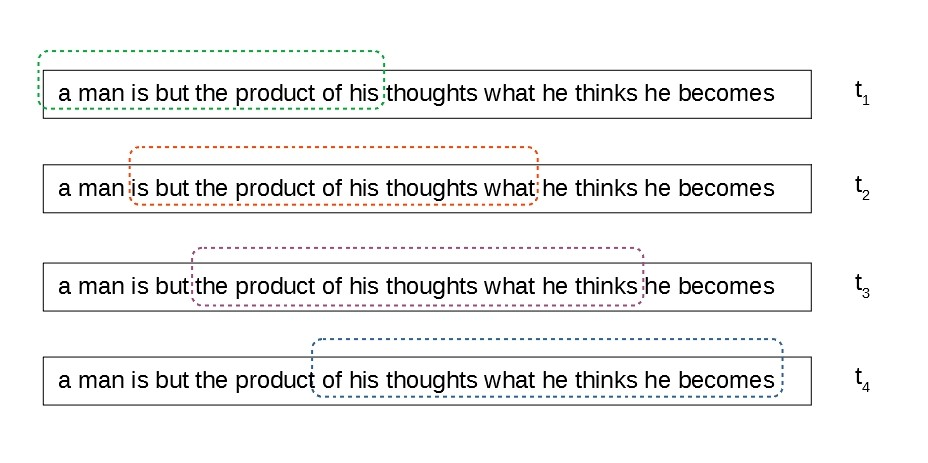
\includegraphics[width=12cm]{pics/SlidingWindow.jpg}
    \captionsetup{justification=centering,margin=2cm}
    \caption{Sliding window at time step $t_{1}$, $t_{2}$, $t_{3}$ and $t_{4}$ with the window size of 10 words per sentence and slide of 2 word per sentence per time step}
    \label{fig:sldingwindow}
\end{figure}

\ref{fig:sldingwindow} shows sliding window, with a window size of 10 words per sentence and slide of 2 words per sentence to create four sentences at time step $t_{1}$, $t_{2}$, $t_{3}$ and $t_{4}$. The following is the list of sentences that the algorithm will create with the above mentioned configuration.

\begin{itemize}
    \item Sentence 1 at time step $t_{1}$: a man is but the product of his
    \item Sentence 2 at time step $t_{2}$: is but the product of his thoughts what
    \item Sentence 3 at time step $t_{3}$: the product of his thoughts what he thinks
    \item Sentence 1 at time step $t_{4}$: of his thoughts what he thinks he becomes
\end{itemize}

In the case when there are less words left than the specified length of the window, then the process will halt with the remaining words in the last sentence.

Here, for training LSTM models, the sliding window based approach is used to create sentences out of the document. The length of slide or the resulting sentence is 30 with slide of 10 words. As each document belongs to one class, the sentences are given the same label as the document is, so if  \textbf{Doc A} $\rightarrow$  \textbf{Class 1} then all the sentences of that corresponding document will be labeled as \textbf{Class 1}. This also helps in mitigation of the problem of less data for training as a single document of 1000 if divided into sentence with sliding window then 98 sentence would be created, which means 98 instances of the class rather than 1 single document. 


\section{Evaluation Matrices}\label{backgroundEvaluationMatrices}

The evaluation of a classification model is very essential. Evaluation of a model gives us insights on how the model will if put to use in production. The following is the list of evaluation measures used in this thesis to evaluate the performance of the models. 

In order to evaluate the performance of any multi-class classification model, we need to first understand the \textit{confusion matrix}.

A confusion matrix describes the performance of a classification model on a set of data where true answers for that data is known.


\begin{table}[!ht]
\centering
\begin{tabular}{ll|l|l|}
\cline{3-4}
 &  & \multicolumn{2}{c|}{Actual Values} \\ \cline{3-4} 
 &  & \multicolumn{1}{c|}{\textbf{P}} & \multicolumn{1}{c|}{\textbf{N}} \\ \hline
\multicolumn{1}{|l|}{} & \multicolumn{1}{c|}{\textbf{P}} & True Positive & False Positive \\ \cline{2-4} 
\multicolumn{1}{|l|}{\multirow{-2}{*}{Predicted Values}} & \textbf{N} & False Negative & True Negative \\ \hline
\end{tabular}
\caption{Confusion Matrix}
\label{table:confMatrix}
\end{table}

\begin{itemize}
    \item \textbf{Positive (P)}:Positive condition (e.g. is mango)
    \item \textbf{Negative (N)}:Negative condition (e.g. is not a mango)
    \item \textbf{True Positive (TP)}: Number of samples that were Positive  (\textbf{P}) and identified and as Positive (\textbf{P}) by the algorithm.
    \item \textbf{False Positive (FP)}: Number of samples that were Negative (\textbf{N}) but identified as Positive  (\textbf{P}) by the algorithm.
    \item \textbf{True Negative (TN)}: Number of samples that were Negative (\textbf{N}) and predicted as Negative (\textbf{N}) by the algorithm.
    \item \textbf{False Negative (FN)}: Number of samples that were Positive (\textbf{P}) but identified as Negative (\textbf{N})
\end{itemize}


\subsection*{Accuracy}
Accuracy of is the ratio of number of correctly identified instances of all classes over the total number of instances in the dataset. 
\begin{align}
    Accuracy &= \frac{\text{Number of correct predictions}}{\text{Total number of predictions}}\\
    Accuracy &= \frac{TP+TN}{TP+TN+FP+FN}
\end{align}

Accuracy in case of unbalanced dataset is not a good measure to evaluate the performance of a model (See \ref{backgroundImbalance}). Hence, other evaluation matrices have to be used in order to get the per class performance of a classifier.

\subsection*{Precision}
Informally, precision indicates how many of Positive conditions were identified correctly. Formally, it is the ratio of True Positive (TP) and sum of True Positive (TP) and False Positive (FP).

\begin{align}
    Precision &= \frac{\text{Correctly identified positive conditions}}{\text{Total number of positive conditions}}\\
    Precision &= \frac{TP}{TP+FP}
\end{align}

\subsection*{Recall}
Recall also known as True positive rate is the amount of positive values that are correctly identified, that is the ratio of True Positive (TP) and sum of True Positive (TP) and False Negative (FN)

\begin{align}
    Recall &= \frac{\text{Correctly identified positive conditions}}{\text{Total number of positive prediction by algorithm}}\\
    Recall &= \frac{TP}{TP+FN}
\end{align}

\subsection*{F-measure (F1-Score)}
F-measure is the harmonic mean of the precision and recall. Harmonic mean is one of the several averaging strategies applicable in situation where average of rates is needed. It is expressed in terms of precision and recall as following,

\begin{align}
    \text{F-measure (F1-Score)} &= \left (\frac{precision^{-1} * recall^{-1}}{2}  \right ) \\
    \text{F-measure (F1-Score)} &= 2 * \frac{precision * recall}{precision + recall}
\end{align}

\subsection*{Macro and Micro Averages}

Precision, Recall and F-measure will give us the performance of the classifier on individual classes and to represent the performance of the classifier on the whole dataset we need to average this values across all the classes. The problem with averaging the values of precision, recall and f-measure across all the classes in case of imbalance of the dataset is misleading as it will weigh each class equally even though the number of samples in some classes were higher and the effect of these classes on precision, recall and f-score will be more. 

Consider the following example:
\begin{itemize}
    \item Class A: 5 TP and 5 FP
    \item Class B: 1 TP and 1 FP
    \item Class C: 20 TP and 90 FP
    \item Class D: 10 TP and 10 FP
\end{itemize}

Calculation precision on these classes we get, $P_{A}, P_{B}, P_{D}= 0.5$ and $P_{C} = 0.2$. 
In macro-average, first the individual precision is calculated and then the average is taken \cite{manning2009introduction}, so macro-average is:
\begin{align}
    \text{macro-average precision} = \frac{0.5+0.5+0.5+0.18}{4} = 0.42
\end{align}
The problem is quite clear as class C which is 84\% of the total dataset is represented in the macro-average precision by $\frac{1}{4}$ ratio \cite{manning2009introduction}.

To mitigate this, in micro-average, we sum up all the prediction of all the classes and then compute the average.
So, micro-average precision for the above example would be:
\begin{align}
    \text{micro-average precision} = \frac{5+1+20+10}{10+2+110+20} = 0.2535
\end{align}
%- Allgemeine Wissensgrundlagen des Fachgebiets
%- Spezielle Grundlagen, die für das Verständnis erforderlich sindhttps://www.overleaf.com/project/5bf3df67d5a222068c001d80
%- Rahmenbedingungen für die Arbeit
%- Ausführungen zum Stand des Wissens / der Technik
%Als Leitprinzip gilt: Nur Informationen erwähnen, die
%- später benötigt werden,
%- notwendig sind, um die Arbeit oder ihre Motivation zu verstehen
%Das heißt insbesondere,
%- keine Inhalte aus Lehrbüchern, außer
%- diese werden benötigt, um Problemstellung oder Lösungsweg zu definieren.

%\hint{The first paragraph should be introduction of things that have been already been done and how the things or techniques that I am using in this thesis may or might have helped  in similar situations. }

%\todots
\chapter{Concept}
\label{ch:concept}

This chapter describes in detail the conceptual aspects of this thesis. The concept is divided into three phases, in the first phase data collection and cleaning will be described, in the next phase resampling of data and clustering will be described and in the last phase, description of machine learning models and the evaluation strategies will be described.

\section{Phase 1: Data Collection and Cleaning}
In the first phase, the data collection techniques are desribed in detail, also how and why the data was cleaned in order to make it suitable for machine learning algorithm is described. 

\subsection*{Data Collection}
Legal laws are written to be applicable in various situations. For example, a law for agricultural products may be applicable in situations where trading of goods happens.  High-level categories of multilingual legal documents provided by the European Union help to navigate in the legislative corpus,  they are also comprised of many languages so that can be used by various Nations. The applicability of these legal texts in various situations makes the classification of these texts on the multi-label classification problem.

To answer the question described in , a dataset has to be acquired. There are many datasets available for legal domains. CFPB Credit Card Agreements DB\footnote{http://www.consumerfinance.gov/credit-cards/agreements/}, EUR-Lex Dataset\footnote{http://www.ke.tu-darmstadt.de/resources/eurlex} are some well known datasets for legal domain specific tasks. However, the CFPB credit card agreements database is not available in German language and also it is about one specific topic in the legal domain. The EUR-Lex Dataset is a large dataset available in both English and German, which was scraped from Publication's office of European Union's website \cite{mencia2010efficient}. This dataset consist of 19,348 documents for a single language divided into 201 topics. This dataset was too large to handle as there are 201 classes and given the amount of resources available to scrap, process and train the models. So instead EUR-Lex summaries were selected. This EUR-Lex Summaries\footnote{https://eur-lex.europa.eu/browse/summaries.html} are also from the Publication office of European Union's Parliament. These summaries are the European Union's laws explained and translated into reader-friendly language. They cover 32 topics which correspond to the activity areas of the European Union.These summaries are available in multiple languages. For this thesis, only \textit{English and German} languages are considered due to their availability across most documents and also the amount of resource available for processing and training the machine learning algorithms were limited. The summaries are not available in easy click to download manner and hence it has to be scraped off of the website of European Union's publication office's website. These summaries changes frequently as the laws of the union changes or if a new law is introduced and as stated above these summaries might belong to multiple classes. 

While scraping the summaries, data from both languages need to be scraped together. This ensures that we are not missing out any summary from either of the language. Saving the summaries from different languages separately would create problem of data leaking, which is result of splitting data randomly for training and testing. For example, \textbf{Doc A} which belongs to \textbf{class 1} in English and \textbf{Doc B} which is same but in German. Now, when spitting the data for training and testing \textbf{Doc A} might end up in training set and \textbf{Doc B} might end up in testing set. 

\subsection*{Data Cleaning}\label{ConceptCleaning}

Text data is unstructured and noisy, meaning that it is not organised in a predefined manner and noisy because it contains a lot of information that may not be of any use for the task at hand. These irregularities makes it difficult for a machine learning algorithm to learn from it. Textual data is non-uniform as the structure and content changes from one document to other, due to these non-uniformity's it is difficult to have a single cleaning mechanism for all machine learning problems involving text. For example, a machine learning task that is designed to detect events might need date and time to effectively predict the event, whereas it would be viable to remove them for a sentiment analysis task.

Legal text is different from other text available because of the style, structure \cite{boella2011using} and the use of special characters which exclusive to the legal text. General text preprocessing techniques becomes feeble, hence during preprocessing of legal text special care must be taken. The data set used here is the summarised version of the original legislation, which contains links to the original documents as well as background information about the law and other information that might not contribute anything in the classification process. These chunks of information can be removed but it is particularly hard to remove them as they do not follow any pattern to where they appear in the document. Due to this reason, even though this information will increase the training time, it was not removed due to its demanding effort.

\section{Phase 2: Data Clustering and Resampling}
%\todo{have to mention clustering first and then resampling}
In the second phase, data was first cluster the data, and then applied the resampling techniques in order to prepare the data for training in the next phase.
\subsection*{Data Clustering}
As the initial step after preprocessing the data, the data was divided into $n$ groups. The division was so that all documents $d$ of a category $C_{l}$ will be grouped together in the same cluster $K_{n}$ via must-link constrains.

%\begin{align}
   % C_{t} = U_{S\in I_{l}}d_{S} \Rightarrow \exists!K_{n}  \forall_{S} \in I_{S} : d_{S} \in K_{n}
%\end{align}

To put it simply, each category $C_{l}$ consisting of documents $d_{s}$ among all other instances with the corresponding class labels $I_{l}$, hence there is only one cluster $K_{n}$ which will have all the instances of the same class (must-link constraints). Each document will be assigned to the closest cluster without violating the must-link constraints. To achieve this, a constrained version of k-means algorithm was applied (see \ref{constrainedKMeans}). Only must-link constraints were available to us in the form of class labels, as each document would belong to one of the 32 classes, however cannot-link constraints, can not be obtained as we do not posses this information or have any prior knowledge about which two documents will not belong together. 

When splitting the data in this manner, the number of classes to be predicted by each multi-class classifier of a cluster is reduced, thus resulting in specialization advantages for each classifier. However, the final classification depends on the results of the previous steps. Each classifier in the chain introduces errors and has less data for training. The classification problem is changed because each classifier has only a subset of classes to predict. Even though the amount of training instances is reduced, the performance effect can still be higher compared to a single multi-class classifier

\subsection*{Data Resampling}

As in many real world applications, data is in skewed distribution and EUR-Lex summaries are no exception. Skewed distribution is when we have more samples in one class then others \cite{wang2012multiclass}. Skewed distribution also know as class imbalance in data is a difficult situation for classifier to learn from as the classifier are biased towards the majority classes and shows poor performance on minority classes. Also, the performance of these classifiers is evaluated using accuracy, which is not a good metric to evaluate the performance of these classifier \cite{chawla2002smote}.  

To handle the imbalances in the dataset various techniques have been proposed. \textit{Oversampling} and \textit{Undersampling} are the two most common ones. Oversampling refers to the process of increasing the number of instances in the minority classes and Undersampling is when we remove instances from the majority class to even out the dataset. Undersampling in our case would mean that we reduce the instances from the majority classes which are as it less to being with. For oversampling the domain specific and limited dataset, I could not find works using artificial techniques such as SMOTE to enhance the data. 
\todo{SMOTE visual on 90 10 dataset}

The EUR-Lex summaries are multi-label, this is generally the case with legal text as a single case may be applicable in many situations. So having multiple labels for a single document can be exploited to alleviate the problem of class imbalance. The sampling of the documents is done in such a way that it reduces samples from the majority classes on the bases of its presence in the minority classes. Hence, a document will be labeled with the class with fewest examples. 

The resampling technique can be better understood with the following example. Consider the dataset in the \ref{table:exampleDataResampling} and the distribution of samples across classes in \ref{table:SamplesDistributionDataResamplingExample}

\begin{table}[!ht]
\centering
\begin{tabular}{cc}

\hline
\textbf{Doc ID} & \textbf{Class Label} \\ \hline
Doc A           & 1,5,2                \\ 
Doc B           & 3,2,5                    \\ 
Doc C           & 4,1,5                  \\ 
Doc D           & 2,3                    \\ 
Doc E           & 2,5                  \\ \hline
\end{tabular}
\captionsetup{justification=centering,margin=2cm}
\caption{An table showing documents and their assignments in their respective classes}
\label{table:exampleDataResampling}
\end{table}

\begin{table}[!ht]
\centering
\begin{tabular}{cc}
\hline
\textbf{Class ID} & \textbf{Number of Samples} \\ \hline
1                 & 2                         \\ 
2                 & 4                          \\ 
3                 & 1                          \\ 
4                 & 1                          \\ 
5                 & 4                         \\ \hline
\end{tabular}
\captionsetup{justification=centering,margin=2cm}
\caption{Distribution of samples in the dataset across 5 classes}
\label{table:SamplesDistributionDataResamplingExample}
\end{table}

When applying the proposed resampling technique to the dataset in \ref{table:exampleDataResampling} and  \ref{table:SamplesDistributionDataResamplingExample}, $Doc$ $A$ which has label 1,5 and 2 will be assigned class 1, similarly $Doc$ $B$ will be assigned to class 3, $Doc$ $C$  to class 4, $Doc$ $D$ to class 2 and $Doc$ $E$ to either 2 or 5. \ref{table:exampleDataResampling} will become

\begin{table}[!ht]
\centering
\begin{tabular}{cc}

\hline
\textbf{Doc ID} & \textbf{Class Label} \\ \hline
Doc A           & 1                \\ 
Doc B           & 3                    \\ 
Doc C           & 4                  \\ 
Doc D           & 2                   \\ 
Doc E           & 2 or 5                  \\ \hline
\end{tabular}
\captionsetup{justification=centering,margin=2cm}
\caption{Document assignment after proposed resampling}
\label{table:exampleDataResamplingAfterResampling}
\end{table}
\clearpage
\begin{table}[!ht]
\centering
\begin{tabular}{cc}
\hline
\textbf{Class ID} & \textbf{Number of Samples} \\ \hline
1                 & 1                        \\ 
2                 & 1 or 2                          \\ 
3                 & 1                          \\ 
4                 & 1                          \\ 
5                 & 0 or 1                         \\ \hline
\end{tabular}
\captionsetup{justification=centering,margin=2cm}
\caption{Distribution of samples in the dataset across 5 classes after resampling}
\label{table:SamplesDistributionDataResamplingExampleAfterResampling}
\end{table}

In \ref{table:SamplesDistributionDataResamplingExampleAfterResampling} class 5 becomes either 0 or 1

This method of resampling has its own limitation. As the samples from majority class is removed and only kept in minority class, the majority class is loosing information about that sample. If the data in a class is diverse, that is, if every sample of that class is unique then applying this technique would result into loss of a that unique representation of the class.


\section{Phase 3: Model Architecture and Training}\label{sec:conceptRQ}
The third phase goes into details regarding the conceptual aspect of the three research questions. It will also detail how the dataset was created for all the research question and what all evaluation strategies were employed for comparison. 

\subsection{Research Question 1:} \label{question1}
The first research question is:
\begin{quote}
    Can \textit{Bidirectional LSTM} achieve better results in terms of evaluation metrics (Precision, Recall and F-Score) than the thoroughly studied text classification methods such as \textit{Support Vector Machines}?
\end{quote}

\ref{fig:FlowResearchQuestion1} shows the approach employed for the above mentioned research question. After the acquiring data from EUR-Lex website, the data was cleaned or prepossessed (see \ref{ConceptCleaning}). Upon preprocessing, the textual data needs to be converted using suitable text representations technique according to the algorithm it will be trained on. Here, there are two algorithms being tested, Support Vector Machines (SVM) and Bidirectional LSTM, and both of them employ different techniques to represent text for training (See \ref{backgroundTextRepresentation}). SVM uses TF-IDF representation whereas LSTM uses Word Embeddings. 
 
Due to hardware limitations training Bidirectional LSTM is difficult if the length of a single instance is very long. Hence each document was divided into sentences using sliding window technique (See \ref{backgroundSlidingWindow}) and document label were assigned to each sentence created from that document. 

\begin{figure}[!ht]
    \centering
    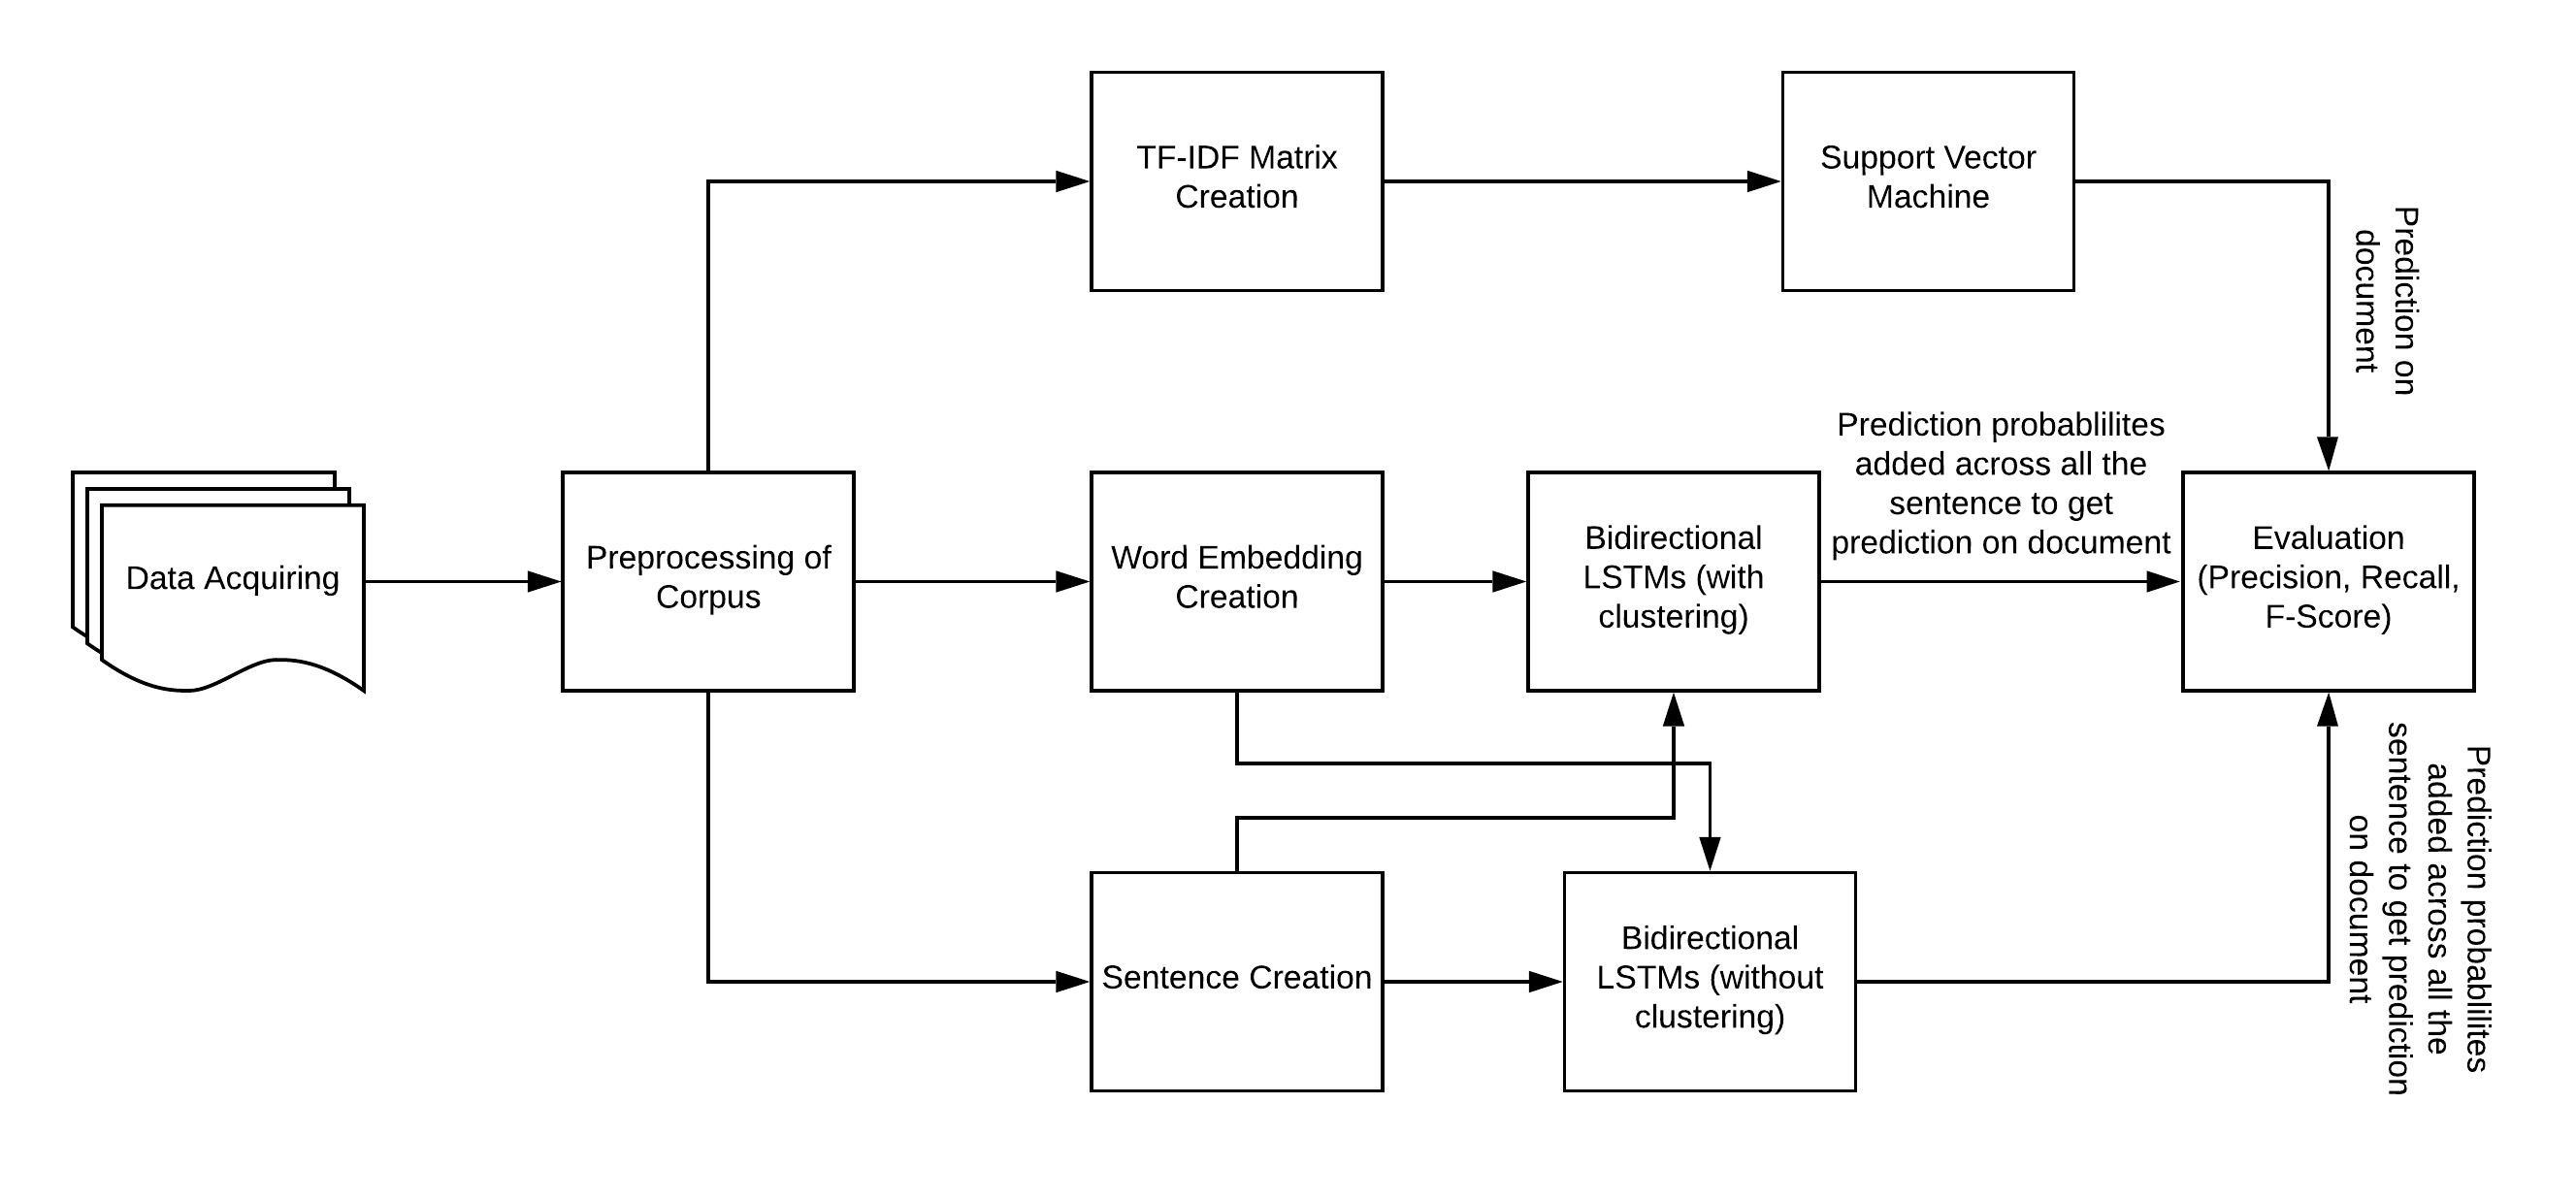
\includegraphics[width=15cm, height=14cm,keepaspectratio]{pics/flowforQuestion1.jpeg}
    \caption{Flow chart representing the workflow for the first research question }
    \label{fig:FlowResearchQuestion1}
\end{figure}

Two LSTM models are trained to see the effects of clustering. The training workflow for the Bidirectional LSTM (with clustering) is shown below in \ref{fig:clusterFlowClassification},

\begin{figure}[!ht]
    \centering
    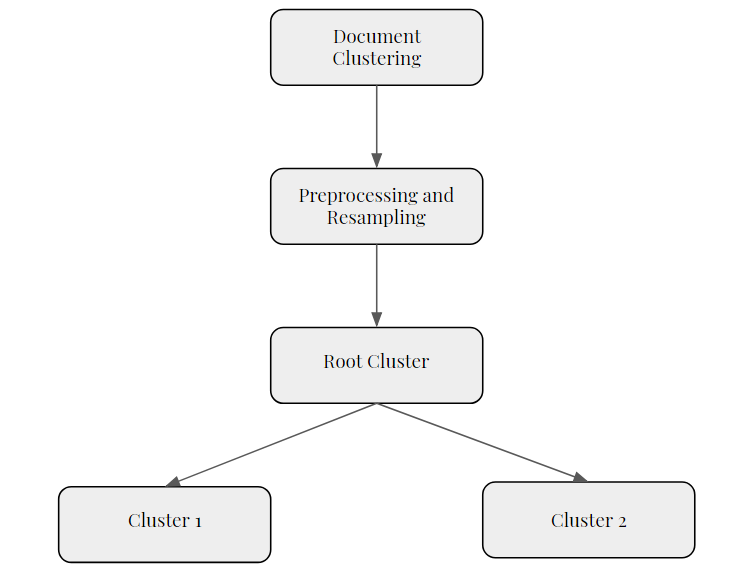
\includegraphics[width=10cm,keepaspectratio]{pics/clusterClassificationFlow.png}
    \caption{Classification workflow for clustered data}
    \label{fig:clusterFlowClassification}
\end{figure}

\subsubsection*{Evaluation} \label{evaluationQuestionOne}
The SVMs are trained on full documents and the LSTMs are trained on the sentences created using the  sliding window technique, for this reason, the results from both the models can not be compared. Ferguson et al.,(2009) \cite{ferguson2009exploring} preformed sentiment analysis of the financial blogs on paragraph-level 
annotated text, they summed up the predictions given by the classifier. In our case, the classifier will give probability to each sentence belonging to each class. As each document comprises of sentences, if we add all the probabilities for each class across all the sentences of a document we get probabilities of each class for that document and then we choose the class with highest probability.
\clearpage
\subsection{Research Question 2:} \label{question2}
The second research question is:

\begin{quote}
    Are general-purpose resources such as \textit{pre-trained word embeddings} in case of \textit{LSTM} applicable to specific legal domain tasks in terms of evaluation metrics? Also, further training them on legal corpus, produces comparable results to the ones only trained on legal texts?
\end{quote}

\begin{figure}[!ht]
    \centering
    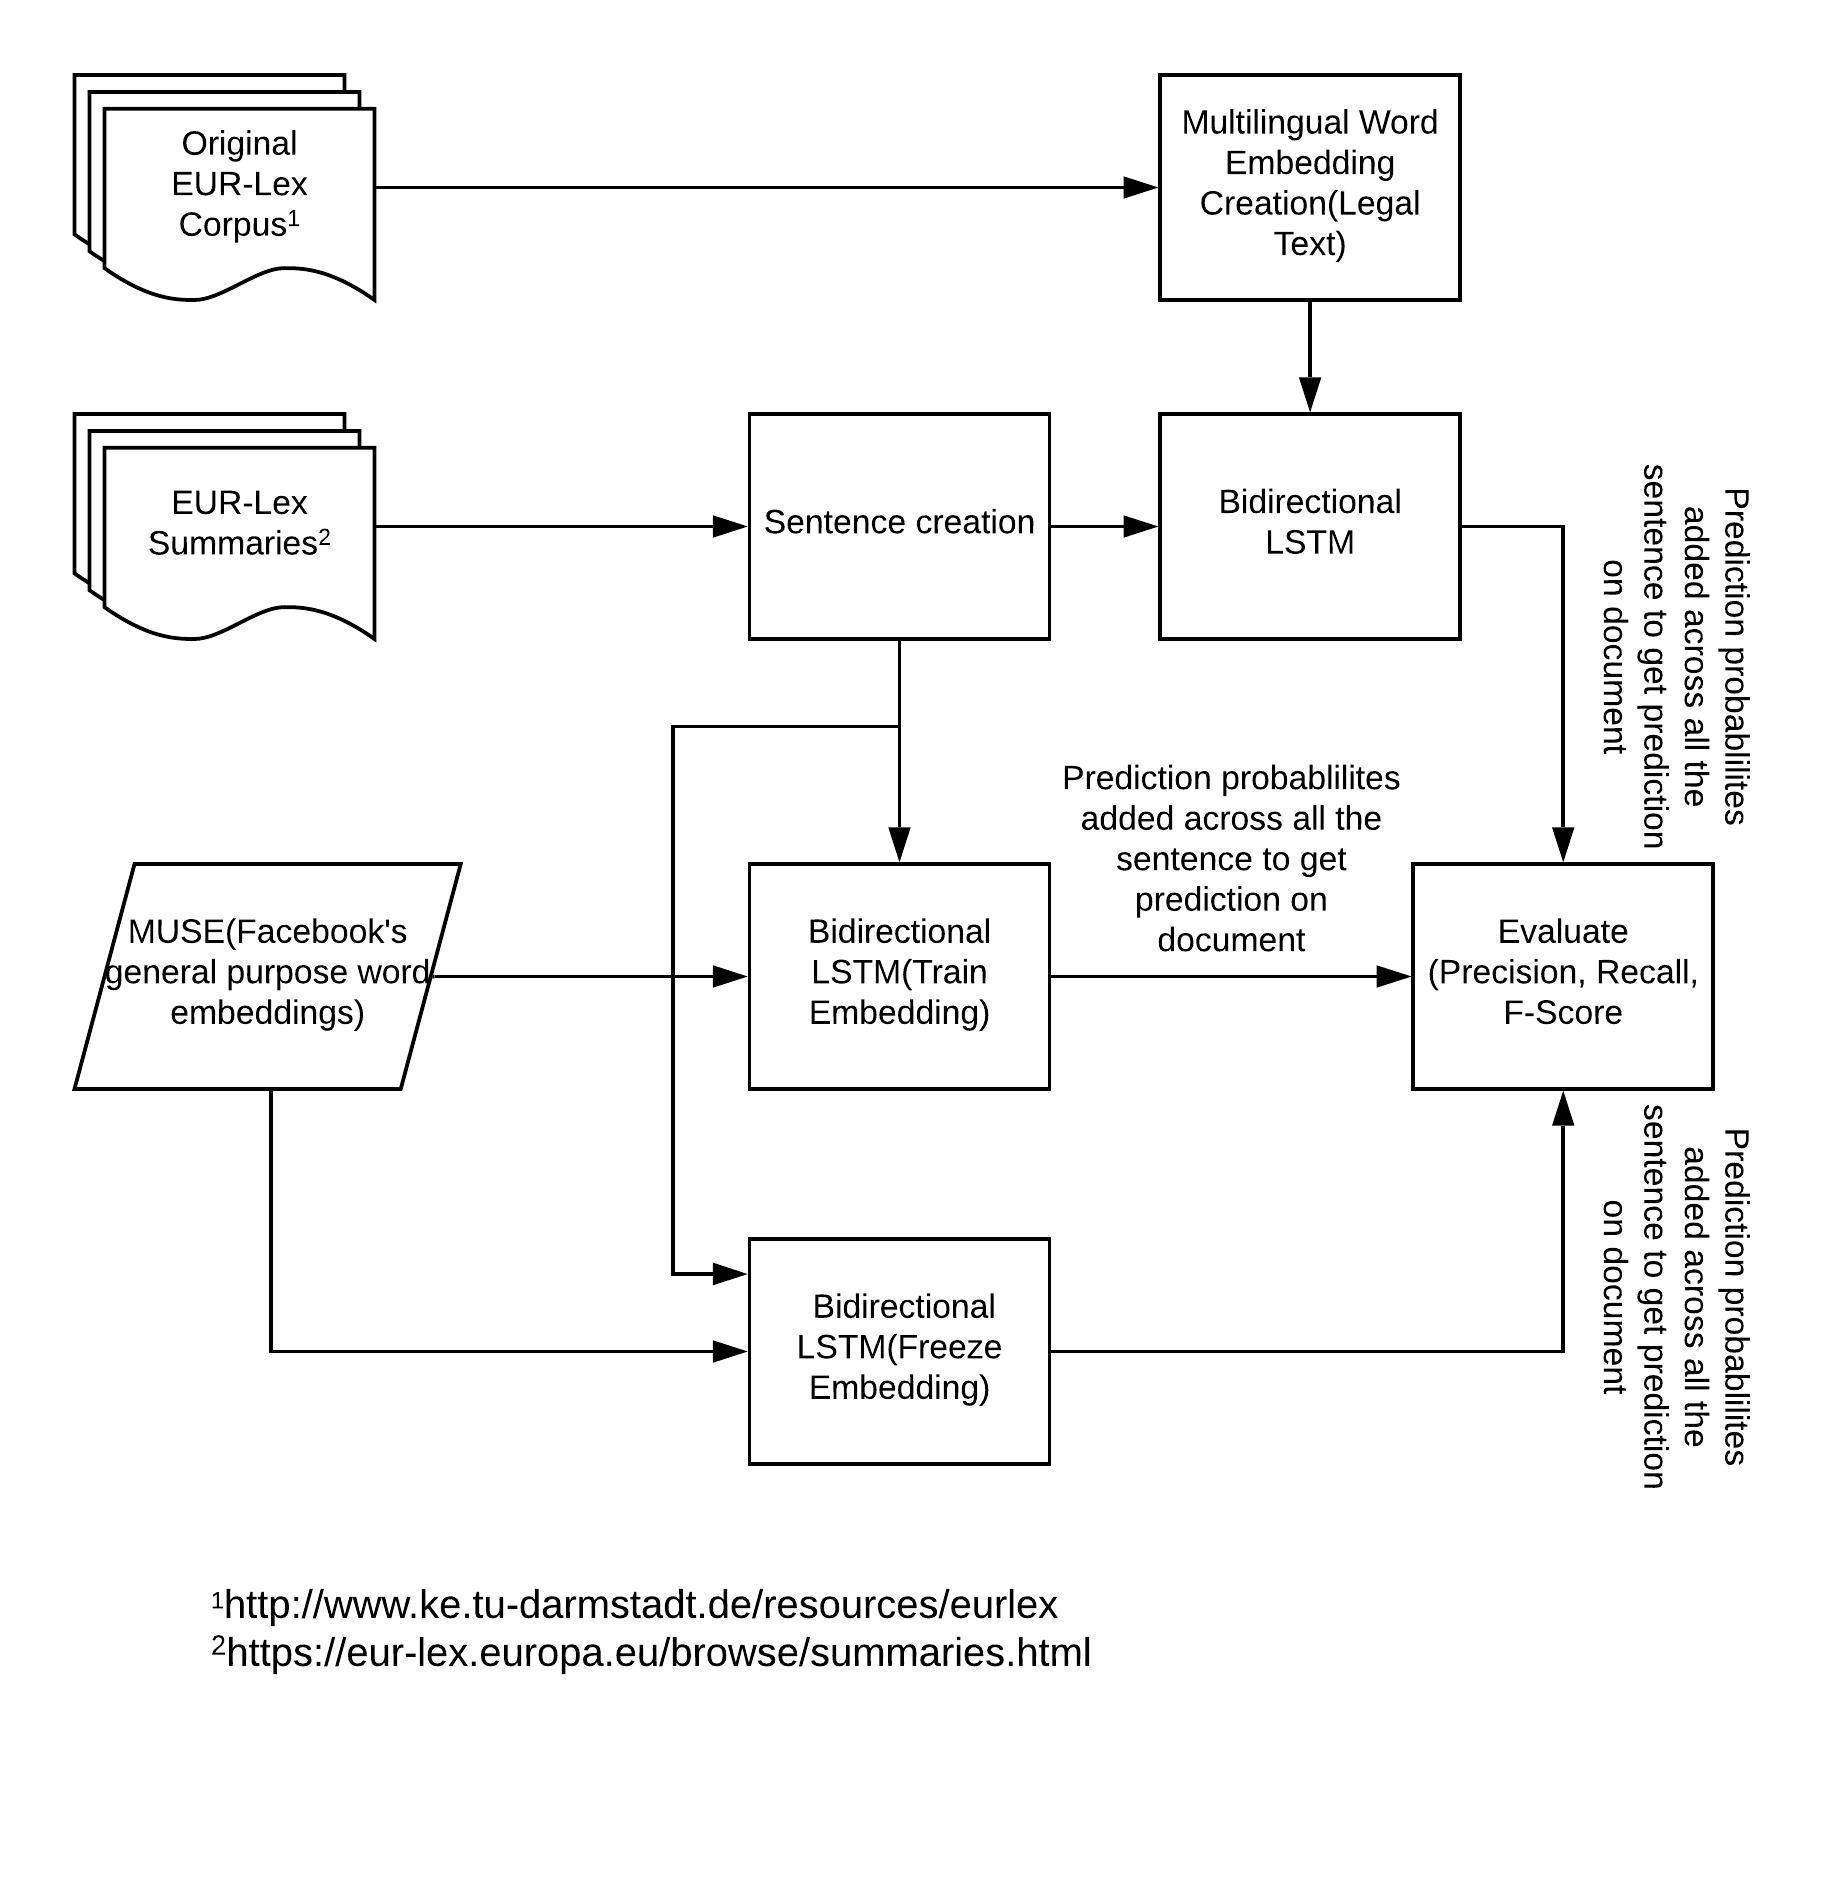
\includegraphics[width=15cm, height=14cm,keepaspectratio]{pics/flowforQuestion2.jpeg}
    \caption{Flow chart representing the workflow for the second research question}
    \label{fig:FlowResearchQuestion2}
\end{figure}

\ref{fig:FlowResearchQuestion2} shows the general workflow for the second question we compare the general purpose resources, that is word embeddings for training LSTM, with the word embeddings trained on legal corpus. Facebook's Fasttext\footnote{https://fasttext.cc/docs/en/crawl-vectors.html}\cite{graves2009novel} provides word vectors in 157 languages on Wikipedia\footnote{https://www.wikipedia.org/} and Common Crawl\footnote{http://commoncrawl.org/} data and is trained using Continuous bag-of-words model in dimension 300, with character n-grams of length 5, a window of size 5 and 10 negatives. But as the word embeddings for multiple languages can not be combined together because they belong in different vector space. Facebook's MUSE\footnote{https://github.com/facebookresearch/MUSE} \cite{conneau2017word} with help of parallel dictionaries was used to align them in a single vector space. After this both embeddings can be simply concatenated and can be used for classification purpose. These word embeddings are created from various sources, it contains text from various domains and hence it will henceforth be refereed to as general purpose word embeddings.

For creating domain specific word embeddings Duong et al.(2016)\cite{duong-EtAl:2016:EMNLP} proposed learning bilingual word embedding without without bilingual Corpora\cite{duong-EtAl:2016:EMNLP}. They also make use of parallel bilingual dictonaries and use Continuous bag-of-word model to create these embeddings. These word embeddings are however in a single vector space.

As the domain specific word embeddings are create using legal domain specific data this word embedding will not be further trained. In case of general purpose word embeddings two models will be trained - one with frozen embedding layer and other model will train the word embeddings. This is done to see if training the general purpose word embeddings produces results comparable to the ones trained on legal data.

Similar to the first question all the models will be trained on clustered data as shown in \ref{fig:clusterFlowClassification} and the as all the models are trained on same data and in same fashion, evaluation will also be done on sentence level and on document level similar to question 1 (See \ref{evaluationQuestionOne}).

\subsection{Research Question 3:} \label{question3}

The third research question is:

\begin{quote}
    Can \textit{LSTM} perform better when training multiple languages in single model, compared to training one model for each language separately?
\end{quote}

\ref{fig:FlowResearchQuestion3} shows the general workflow for the third research question. In this question we explore the possible effects of having data in multiple languages on a classifier. C.-P. Wei et al.(2014)\cite{Wei:2014:EPD:2566999.2567111} suggested that when the training set for a single language is small it is less representative of the target semantic space and a classifier trained on this data set would not yield satisfactory results. However, if the text from another language is available for the predefined category then it can be beneficial and can improve the effectiveness of the classifier for the previous language. The naïve approaches of handling such data is to build separate classifiers for separate languages. This naïve method does not take the benefit of availability of data across different language for a defined category. 

In this research question, first two separate classifiers will be trained on two different languages namely, \textit{English} and \textit{German}. The results from both of them will be combined to get the average performance (we will average the macro-average precision, recall, and f-score across both the models) of classification of these two classifiers. The training and evaluation of these classifiers will be similar to the training done in question 1 and 2. This performance of the two classifiers will then be compared to a single classifiers that will be trained on both the languages with multilingual word embeddings.

The training of all the classifiers for this question will be done in the similar fashion as show in \ref{fig:clusterFlowClassification}.


\begin{figure}[!ht]
    \centering
    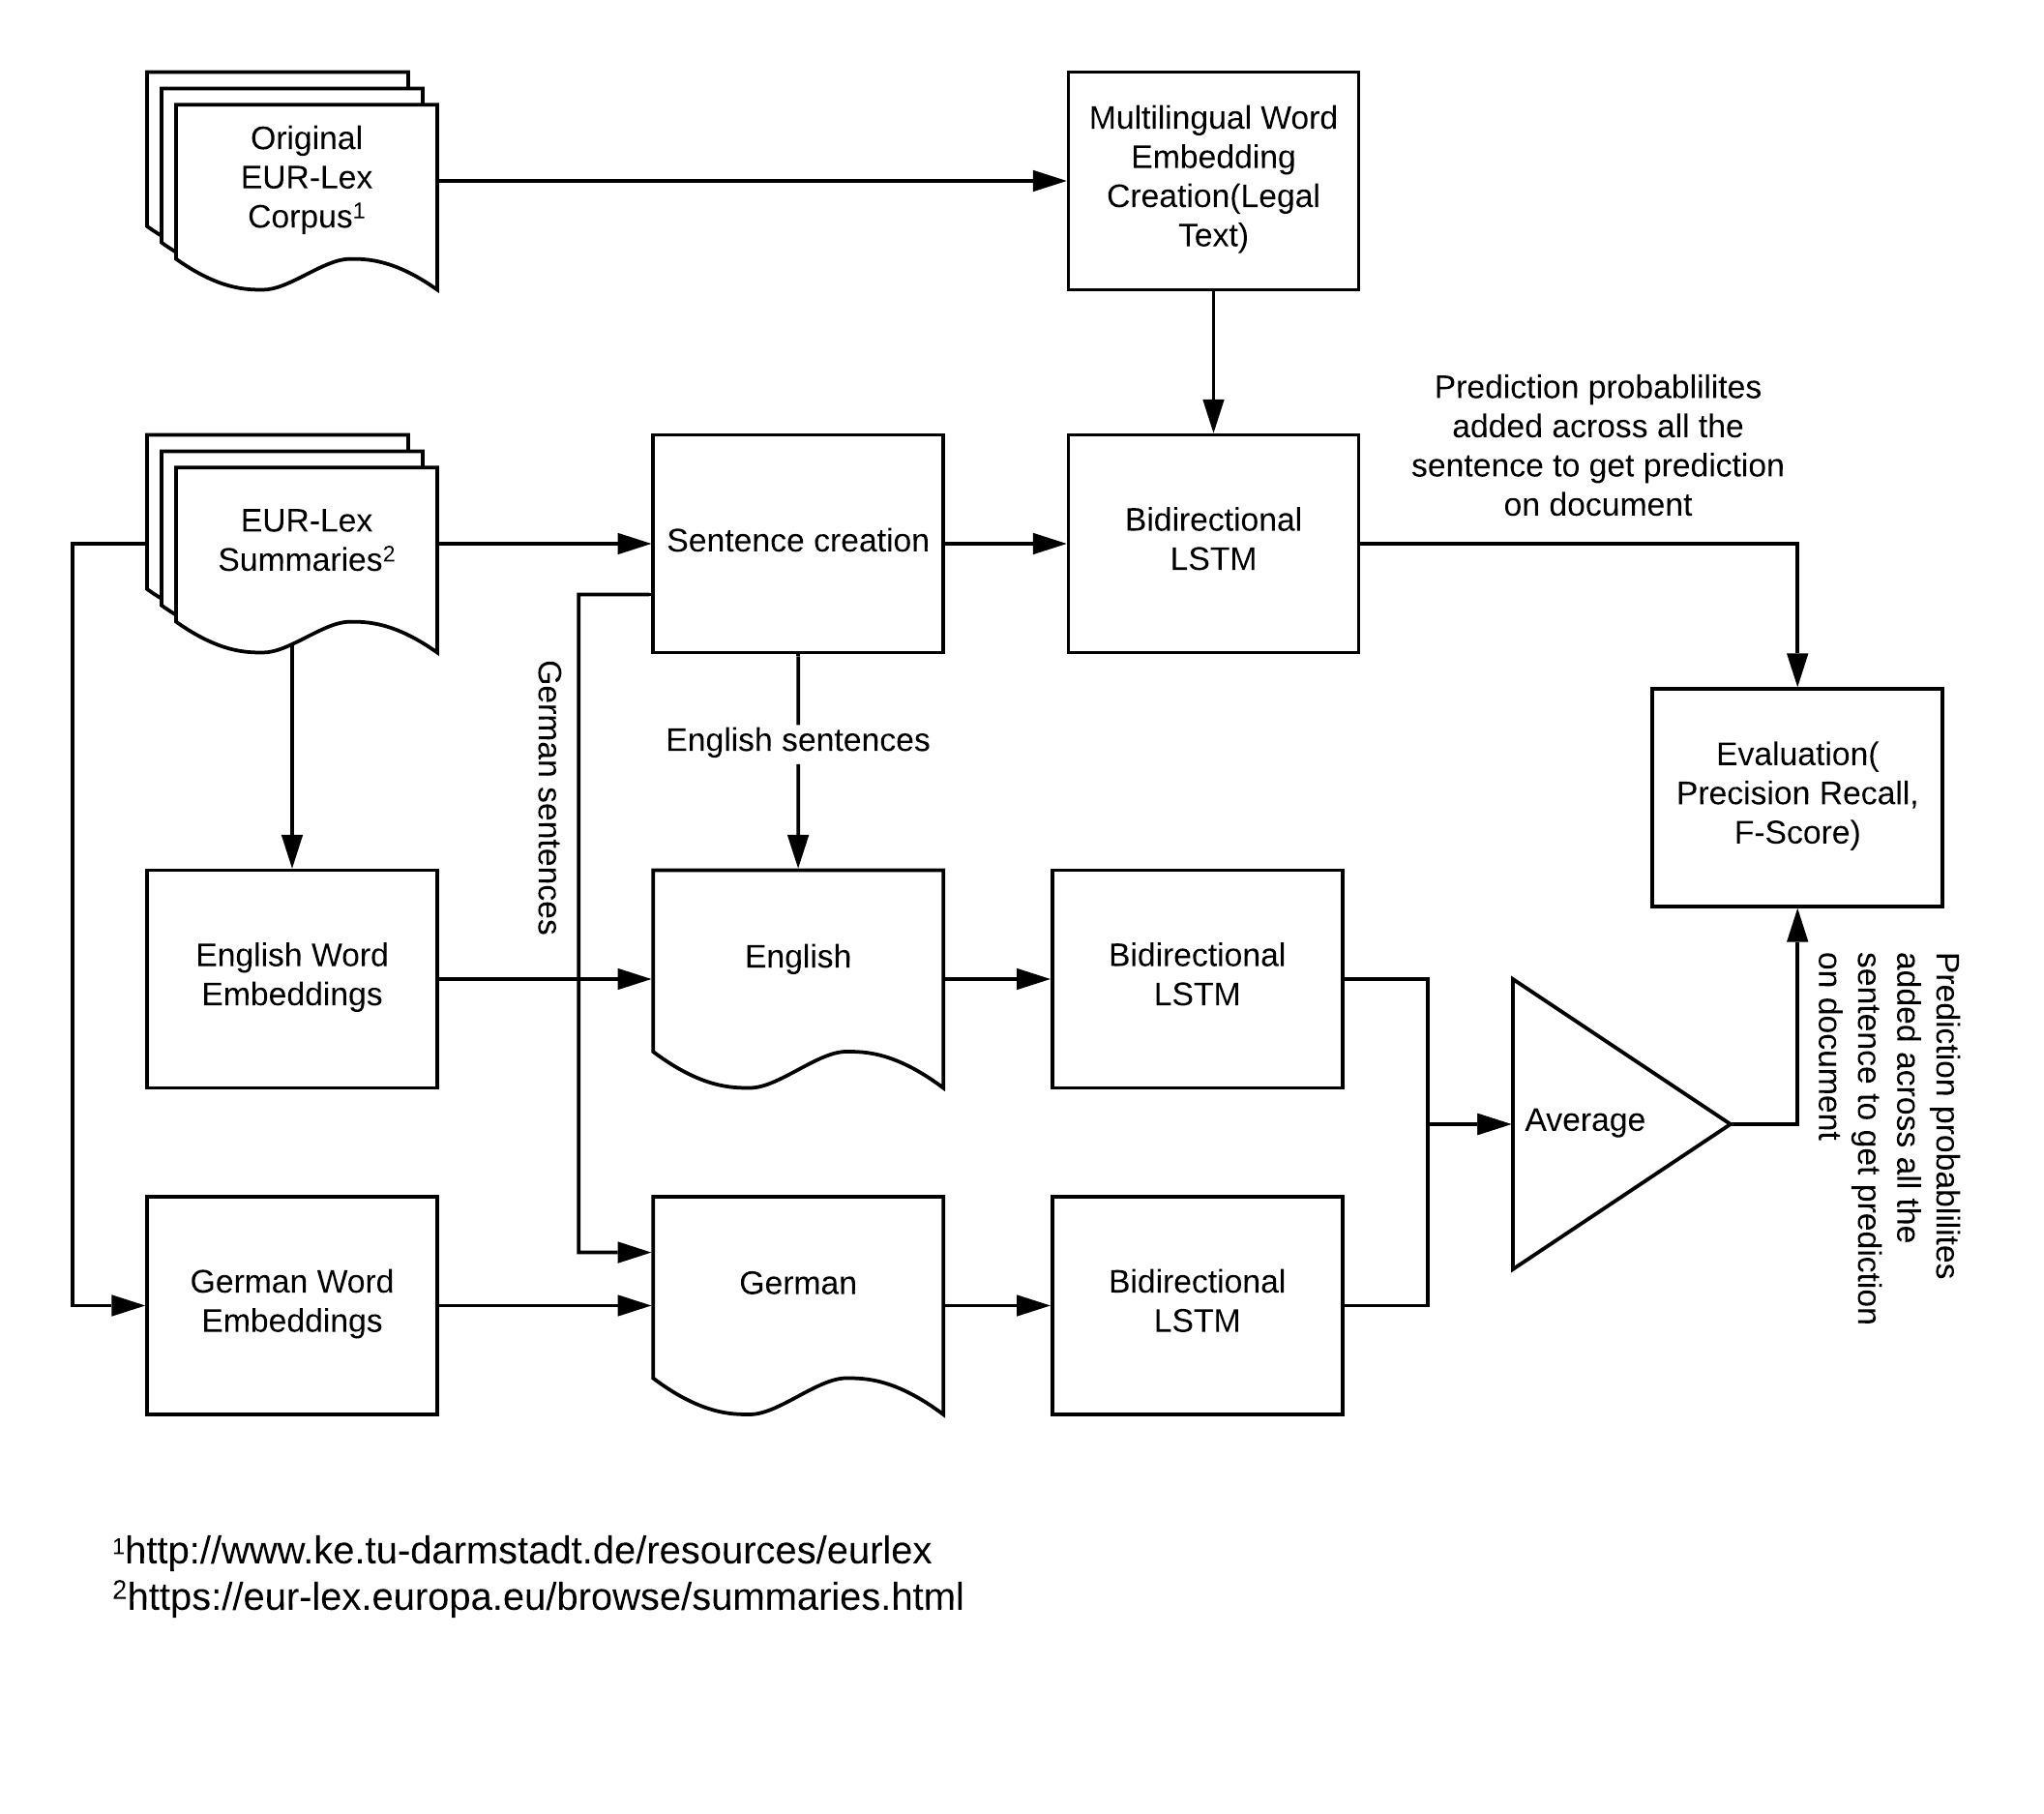
\includegraphics[width=15cm, height=14cm,keepaspectratio]{pics/flowforQuestion3.jpeg}
    \caption{Flow chart representing the workflow for the third research question}
    \label{fig:FlowResearchQuestion3}
\end{figure}

For the evaluation, the multilingual classifier is evaluated on summation of predictions from the sentences of each document for each class. Also, both of the monolingual classifiers will be evaluated on summation of the predictions from the sentences of each document of each class but these results will then be averaged to be able to compare it with the multilingual classifier also to see how they perform on sentence level the evaluation will also consider the results on sentence level.


\ifgerman{\chapter{Implementation}}{\chapter{Implementation}}

This chapter describe in detail about how data was collected, what preprocessing techniques were applied to the data in order to make it fit for machine learning algorithm to learn from, how data was resampled in order to balance it to some extent, how it was clustered and what are the details of the architecture of the models and what are the evaluation strategies applied.

\section{Data Collection}
To begin with the implementation, the first step was to obtain the data. Obtaining the data was particularly  challenging as these summaries were frequently changing, so scrapping the data at different times results in different assignment of a single document in different categories. Also another challenge was that when documents for English and German were scraped separately, it happened quite often that some documents from one language were missing. Due to these challenges, a carefully crafted scraper which scrapes the data only if documents from both the languages are available, this in turn added a time overhead. Even after those considerations, there were some documents missing from one of the language.

For scrapping the data Python library \textit{Beautiful Soup} and \textit{urllib} was used. 

\section{Data Cleaning}\label{preprocessing}

The preprocessing involved removing of \textit{punctuation's}, \textit{numbers}, \textit{currency symbols} as they do not contribute anything in the classification process. The next step is to normalize the text, this step is necessary because of the \textit{inflection} added due to the modification of words.

%\todo{A figure explaining how played, plays and playing is all from the root word \textit{play} }
Stemming and Lemmatization are two techniques used to normalize the text. Both techniques reduces words to its root form. Stemming reduces the word into base but this base may or may not be the morphological root of the word. It should suffice that the related words are mapped to the same base, even if the base is not a valid root. For example, words \textit{argued}, \textit{arguing}, \textit{argue} and \textit{argues} will all be stemmed to \textit{argu}, even though the base \textit{argu} is not a valid term in itself. The process of stemming is more heuristic. It removes affixes such as \textit{-ed,-ize, -s,-de} without taking into account that the base might not be a word in the same language. On the contrary lemmatization reduces the words by ensuring that the base belong to the language. The base word in lemmatization is called a \textit{lemma}. Lemmatization is necessary in the cases where it is necessary to get valid words.This will be clear in the coming section of word embeddings. This is the reason, that instead of stemming, lemmatization is used as word normalization technique.  \todo{example of lemmatization and stemming comparision}

As the last step, \textit{stop words} from both the languages were removed because, first they don't contribute anything, second they increase the training time of the algorithm. For German language, \textit{umlauts - ä, ö and ü} are converted into its base form that is \textit{ä to ae, ö to oe and ü to ue.}

Following are the steps in which the preprocessing was done.

\begin{enumerate}
    \item As a first step, \textit{stop words} are removed.
    \item Next step is to lemmatize the words.
    \item Removal of other unnecessary symbols are removed. For example, § is symbol of paragraph and is extensively used in legal text. • is also another example.
    \item Remove numbers
    \item Punctuation removal
\end{enumerate}

The order of the steps is also important as it will help in reducing the overload on some of the processes. For example, when the stop words are removed in the first step, then the lemmatizer would not have to go through those words and that will decrease the time taken to process the text. There were other Unicode characters which were also removed. 

\subsection{Data Preprocessing for pretrained word embeddings}
Pretrained language models are trained on large corpora and hence they can be used for variety of task in natural language processing. These models are trained on corpora that have no specific domain. Legal text is different from the corpora these models are trained on such that the words we find in legal text are rarely used outside the legal domain. 

For the scope of this thesis, to answer the question \textit{"Can general purpose resource be used for legal domain specific task?"} I am going to use Facebook's MUSE multilingual word embeddings \cite{conneau2017word}. These word embeddings are created by learning a mapping between the two sets of monolingual word embeddings.\todo{have to write what methods were used to create these} The monolingual word embedding used in were created using fastText \cite{bojanowski2017enriching}. These pretrained vectors were trained on Common Crawl and Wikipedia Coprus. There was no preprocessing involved except for lower casing the words. Hence, to use these word embeddings, I need to use the corpus with only lower case words and avoid all the preprocessing mentioned in the section in order to have the classifier learn better. If the preprocessed data is used with the embedding that were created using non processed data then even if the 


\section{Data Resampling} \label{dataResampling}
The EUR-Lex summaries, are the summarised versions of legislations. These summaries are written in an abstract manner to apply for multiple situations, so that one regulation may belong to several categories. Multi-label classifier with very few examples might not be applicable as the classifier will favour majority class because of the imbalance. 

From \ref{graph:distribution of data english docs} it is clear that the data suffers from class imbalance. To mitigate the problem of class imbalance we upsample minority class or downsample majority class. In our case, upsampling minority class is difficult as it is very hard to produce alike documents because of nature of text and downsampling minority class would lessen the already less data. We had to find a way to not only downsample the majority in such a fashion that would result into balancing the data as well as not lessen the data to an extent that is not useful anymore.
\todo{give an example to make it clear}
As the data is multilabeled it can be exploit because of the fact that a sample might belong to more than one class. The documents are transformed in such a way that if a document belongs to two or more class, then it will be kept in the class with minimum number of samples. That is the class label for that document will be the one with the fewest examples. This method will downsample the majority class as only the duplicated documents are removed from it but also make this classification problem a multi-class from a multi-label one. In the testing phase, the predictions are allowed from the set of all the true labels. This method however introduces a bais towards the minority classes but it acknowledges the presence of other possible category assignment in the end result.

\begin{figure}[!ht]
\begin{center}
\makebox[2pt]{
\begin{tikzpicture}
  \centering
  \begin{axis}[
        ybar, axis on top,
        title={},
        height=4cm, width=14cm,
        bar width=0.1cm,
        ymajorgrids, tick align=inside,
        enlarge y limits={value=.1,upper},
        ymin=0, ymax=700,
        axis x line*=bottom,
        axis y line*=left,
        y axis line style={opacity=0},
        tickwidth=0pt,
        ytick style={draw=none},
        enlarge x limits=true,
        legend style={
            at={(1,1)},
            anchor=north east,
            legend columns=-1,
            /tikz/every even column/.append style={column sep=0.5cm}
        },
        ylabel={number of documents},
        symbolic x coords={
        agriculture,
        audiovisual  and  media,
        budget,
        competition,
        consumers,
        culture,
        customs,
        development,
        economic  and  monetary  affairs,
        education  training  youth,
        employment  and  social  policy,
        energy,
        enlargement,
        enterprise,
        environment,
        external  relations,
        external  trade,
        fight  against  fraud,
        food  safety,
        foreign  and  security  policy,
        human  rights,
        humanitarian  aid,
        information  society,
        institutional  affairs,
        internal  market,
        justice  freedom  security,
        maritime  affairs  and  fisheries,
        public  health,
        regional  policy,
        research  innovation,
        taxation,
        transport
        },
       xtick=data,
       x tick label style={rotate=90,anchor=east},
       %nodes near coords={\pgfmathprintnumber[precision=0]{\pgfplotspointmeta}}
    ]
    \addplot [draw=none, fill=blue!30] coordinates {
        (agriculture, 37)
	    (audiovisual and media,54) 
		(budget,36) 
		(competition,101) 
		(consumers,190) 
		(culture,44) 
		(customs,60) 
		(development,164) 
		(economic and monetary affairs,160) 
		(education training youth,190) 
		(employment and social policy,427)
		(energy,150)
		(enlargement,168)
		(enterprise,106)
		(environment,380)
		(external relations,149)
		(external trade,69)
		(fight against fraud,64)
		(food safety,166)
		(foreign and security policy,64)
		(human rights,54)
		(humanitarian aid,45)
		(information society,136)
		(institutional affairs,179)
		(internal market,296)
		(justice freedom security,544)
		(maritime affairs and fisheries,96)
		(public health, 79)
		(regional policy,120)
		(research innovation,98)
		(taxation,16)
		(transport,309)  };
   \addplot [draw=none,fill=red!30] coordinates {
      (agriculture, 32)
(audiovisual and media, 24)
(budget, 32)
(competition, 86)
(consumers, 131)
(culture, 41)
(customs, 54)
(development, 99)
(economic and monetary affairs, 148)
(education training youth, 148)
(employment and social policy, 222)
(energy, 116)
(enlargement, 103)
(enterprise, 89)
(environment, 161)
(external relations, 104)
(external trade, 57)
(fight against fraud, 41)
(food safety, 116)
(foreign and security policy, 59)
(human rights, 54)
(humanitarian aid, 39)
(information society, 89)
(institutional affairs, 150)
(internal market, 192)
(justice freedom security, 320)
(maritime affairs and fisheries, 89)
(public health, 63)
(regional policy, 100)
(research innovation, 91)
(taxation, 67)
(transport, 193) };
\legend{Original, Resampled}
\end{axis}
\end{tikzpicture}
}
\end{center}
\captionsetup{justification=centering,margin=2cm}
\caption{Class distribution of the EUR-Lex summaries corpus, comparing the original
to the resampled distribution.}
\label{graph:originalVSresampled}
\end{figure}


\section{Clustering} \label{clustering}
Document cluster in information retrieval helps in organization, extraction of topic and text, filtering. The idea here was that given the number of classes and the number of documents per classes as it is a unbalanced dataset,it will be difficult for a classifier to learn on this data. 

Clustering of documents was only possible provided that all the documents $d$ of a category $C$ belong only to that category. Also, it is important to find out what is the number $n$ that the documents must be clustered into. The number of clusters $n$ is determined bu silhouette score \cite{rousseeuw1987silhouettes} and elbow analysis \cite{thorndike1953belongs}. 

K-Means cluster is used here to cluster the documents. Splitting the documents this way, the number of classes to be predicted by each classifier is reduced thus, resulting in specialization advantage for each classifier. However, the final classification depends on the classification from previous classifiers, so any error introduced will be propagated downwards. This method of division is can be advantageous as we have $32$ classes and it can be a challenge for a single classifier to learn on them given the amount of data.

\clearpage


\section{Training the Word Vectors}

Conventionally, text representation in natural language processing involves techniques like \textit{Continuous bag-of-words} and \textit{if-idf}. These techniques are simple representation of various features. However, in bag-of-words approach, grammar and word order are not considered. And in tf-idf only importance of words is considered, section \ref{sec:svm}. Hence, techniques does not capture the semantics of the text \cite{maas2011learning}.

\todo{already in backgroud, write about just the training part. How you did it}
Due to the above limitations words vectors are used. Word embeddings are vector representation of meaning of words in the corpus. This means that words are placed in high-dimensional vector space where words with similar meaning are placed close to each other. Neural network based word vector models are usually trained using stocastic gradient descent where gradient is obtained by backpropogation \cite{le2014distributed}. One popular algorithm is \textbf{Word2Vec} \cite{mikolov2013efficient},in this implementation word embedding are trained using two models, Continuous bag-of-word model and Continuous Skip-gram model. In continuous bag-of-words, the projection of words into vector space is not influenced by the order of words and words from future are also used in this model. Unlike, standard bag-of-words it uses continuous distributed representation of context. The architecture is similar to Feedforward Neural Net Language model \cite{bengio2003neural}. In Continuous Skip-gram model, instead of predicting next word based on context, it tries to maximize the classification of next word based on other word in the sentence.

After the network converges, words with similar meaning are placed together. For example words like "powerful" and "strong" are placed closed in the vector space. \todo{Need to work on this, doesn't look good}

The model used in creation of the word vectors is a neural network, and neural networks are data hungry as it requires a lot of data to train them properly. As a result, another domain specific dataset is used in this experiment because dataset used for classification is small. Hence, the whole EUR-Lex dataset was used as it contains 19,348 documents mostly consisting regulations, decisions and directives of European Union \cite{jf:SemanticLaw}.

\subsection{Cross Lingual Word Embedding}
Word vectors for different languages are in different vector spaces, hence it can not be combined together, but the classification task involves classifying text from two languages, \textbf{English} and \textbf{German}. Hence, for classifying both languages within a single model is necessary. This not only mitigates the error caused by a language detector in multilingual systems, where a language detector first detects the language and then the respective classifier is invoked. In that affair, error propagates downwards and amplifies. And using multiple languages also increase the amount of data for training if multilingual parallel corpora is available where corpus of single language is low. 

To achieve this \cite{duong2016learning}, proposed using bilingual dictionaries and monolingual data. The model uses an extension of contextual bag-of-word(CBOW) model \cite{mikolov2013efficient}. This method has benefits as often there no parallel data when working on a domain specific problems, also it is comparatively easy to obtain or create bilingual domain specific dictionaries. \todo{Write about the method}

I will be using the technique suggested by \cite{duong2016learning}. For creating bilingual dictionary, \textit{EuroVoc} thesaurus \cite{steinberger2002cross} provided by Publication office of European Union will be used. It is available in 24 official languages recognised by European Union. This thesaurus is domain specific hence it does not involve common words that might occur in the documents. Due to this reason, this thesaurus is combined with bilingual dictionaries that are available from \textit{Facebook MUSE} \cite{conneau2017word}. This bilingual dictonaries were created using Facebook's internal translation tools. The authors claims that these dictionaries handle the polysemy of the words better. This combined bilingual dictionary with the original EUR-Lex dataset was used to create the legal domain specific bilingual word embeddings. 

For creating General purpose word embedding using the above mention method is time and resource consuming, as a lot of monolingual data needs to be obtained and also large bilingual dictonaries need to be obtained as well. This would also mean that there would be bais in creation of these embeddings as we would have prior knowledge about what works well with algorithms and the data we are using, also this would beat the purpose of comparing General Purpose resources to one created using domain specific resources. Hence, we are using Facebook's MUSE word embeddings \cite{conneau2017word}, the author claims that the embeddings are state-of-art multilingual word embeddings, these word embedding are facebooks fasttext \cite{bojanowski2017enriching} which are aligned in common vector space. They use two sets word embeddings that are trained on monolingual data, and learns the mapping between these two embedding in a common vector space. It exploits the similarities of monolingual embedding space \cite{mikolov2013exploiting} to learn mapping between the two embeddings.
The method used by \cite{conneau2017word} is domain adversarial learning. \todo{this needs to go} In this method a model is trained to discriminate between randomly sampled elements from the two embeddings. For example, let $X$ $=$ ${x_{1}, x_{2}...x_{n}}$ be the first of the two monolingual word embedding, and $Y$ $=$ ${y_{1}, y_{2}...,y_{n}}$ be the second monolingual word embedding. $W$ is trained to block the discriminator making right predictions. 


\section{Architecture and Training}

The case of class imbalance is clear from \ref{graph:distribution of data english docs}. Applying the resampling technique proposed in \ref{dataResampling}, we have mitigated the problem of data imbalance to some extent. The \ref{fig:approach} shows the divide-and-conquer philosophy. This approach assumes that the classifier will benefit from the specialization effect from a small number of classes. \\

\begin{figure}[!ht]
    \centering
    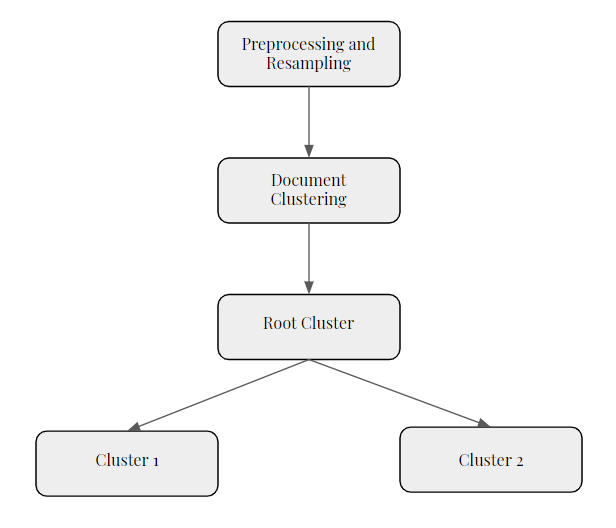
\includegraphics[height=5cm,width=9cm,keepaspectratio]{pics/Approach.PNG}
    \captionsetup{justification=centering,margin=2cm}
    \caption{The workflow of the preparation, resampling and training of the proposed technique.}
    \label{fig:approach}
\end{figure}
\clearpage

First the preprocessing of the documents is done, after that in the resampling phase, class imbalance is tackled to some extent. Then, similar categories are grouped together based on the clustering technique presented in \ref{clustering}. In the data set preparation stage, the English and German documents with labels were pickled together so that during the Train-Test split, no parallel document from either language ends up in both, that is if \textbf{Doc A} from English language and parallel document \textbf{Doc} $\mathbf{\Tilde{A}}$ from German language don't end up in Train set and Test set respectively or vice versa. After ensuring the conformity, the dataset was divided into Train set and Test set with ratio of 70\% and 30\% respectively. This division was done on document level before creating sentences to ensure that sentences from a single document end up in only one of the two sets, This is very important, not conforming to this might create problem of data leakage. Also the train-test split was performed in stratified fashion to ensure that the ratio of number of samples in classes in Train set is same as the ratio of samples of classes in Test set.

















\ifgerman{\chapter{Evaluierung}}{\chapter{Evaluation}}
\label{ch:evaluation}

Evaluating a classification algorithm also known as classification model is necessary to find how competent the algorithm is on data it has never seen. The classification model generates probabilities when given the of predicting on unobserved data. 

\section{Experimental Setup}
Most of the experiments were carried out on \textit{Google Colab} is a free google service that provides Jupyter notebooks with Python environment that stores the notebooks on Google Drive. It provides a GPU (Graphics Processing Unit) or TPU (Tensor Processing Unit) and has pre-installed various popular machine learning and deep learning framework. The exact detail of the system is listed in the \ref{table:HWsetup}

\begin{table}[!ht]
\centering
\begin{tabular}{cc}
\hline
\textbf{Hardware} & \textbf{Specifications} \\ \hline
CPU & 2vCPU Intel(R) Xeon(R) Processors @2.20Ghz \\
GPU & 1xTesla K80 12GB(11.439GB Usable) GDDR5  VideoRAM \\
TPU & \multicolumn{1}{l}{Google's custom developed application-specific integrated circuits} \\
RAM & 12GB \\
DISK & 358.27 GB \\ \hline
\end{tabular}
\caption{Hardware specification for the experimental setup}
\label{table:HWsetup}
\end{table}

All the experiments were performed using \textit{Python 3} environment. \textit{scikit-learn}, an open source machine learning library in Python is used here for data processing and training the SVM. For Bidirectional LSTMs, \textit{Keras} an open source neural network library written in Python is used with \textit{Tensorflow} backend.  

The packages, their version numbers and the purpose are listed below in \ref{tabel:packageList}
\clearpage
\begin{table}[!ht]
\centering
\begin{tabular}{>{\centering\arraybackslash}m{3.4cm}>{\centering\arraybackslash}m{3.4cm}>{\centering\arraybackslash}m{6cm}}
\hline
\textbf{Package Name} & \textbf{Version Number} & \textbf{Description} \\ \hline
scikit-learn & 0.20.3 & An open source machine learning library for data mining and data analysis. \\[0.2cm]
keras & 2.2.4 & An open source neural network library for fast prototyping, uses likes of Tensorflow or Theano. \\[0.2cm]
tensorflow & 1.13.1 & An open source software library for numerical computation using data flow graphs. \\[0.2cm]
beautifulsoup4 & 4.6.3 & A python library for parsing HTML and XML documents. \\[0.2cm]
matplotlib & 3.0.3 & A python library for plotting and visualization. \\[0.2cm]
nltk & 3.2.5 & A python library for statistical Natural Language Processing. \\[0.2cm]
seaborn & 0.7.1 & A python library for statistical data visualization. \\[0.2cm]
spacy & 2.0.18 & An open-source software library for advanced Natural Language Processing. \\[0.2cm]
numpy & 1.14.6 & An python library for creating and manipulating, large and multiple dimensional arrays. \\[0.2cm]
scipy & 1.1.0 & An python library for scientific and technical computing \\ \hline
\caption{List of packages used}
\label{tabel:packageList}
\end{tabular}
\end{table}


\section{Evaluation Approach}
For evaluation, initially 70\% of data is used for training the classification models and then 30\% of the data is used for evaluation. The evaluation is done on sentence 

\begin{figure}[!ht]
    \centering
    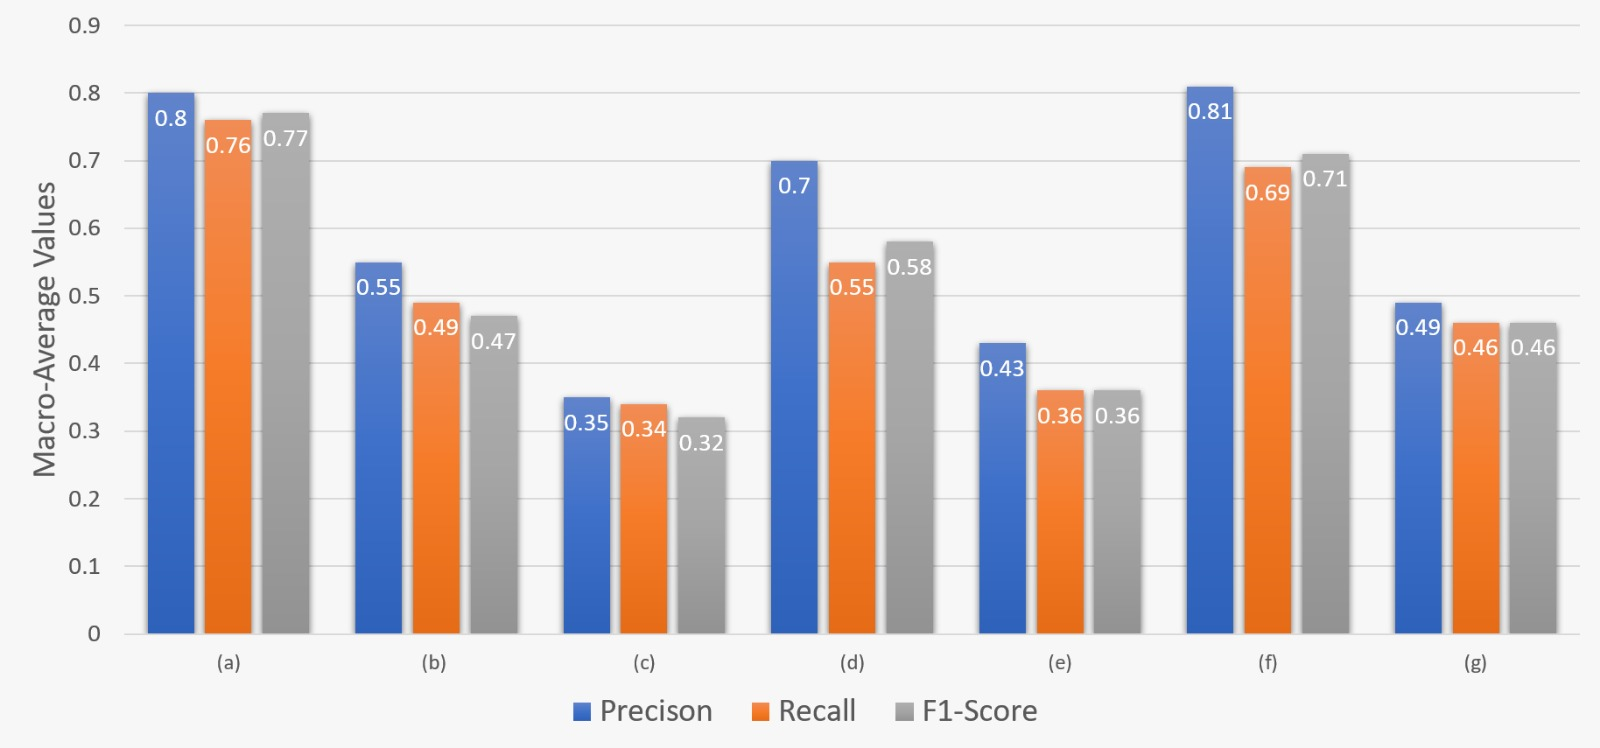
\includegraphics[width=16cm, keepaspectratio]{pics/EvaluationQ1.jpeg}
    \caption{Macro-averaged Precision, Recall and F1-Score of (a) Support Vector Machine on English data, (b) Bidirectional LSTM on English language without clustered data evaluated on document level, (c) Bidirectional LSTM on English language without clustered data, evaluated on sentence level, (d) Bidirectional LSTM on English and German language without clustered data, evaluated on document level, (e)
    Bidirectional LSTM on English and German language without clustered data, evaluated on sentence level, (f)
    Bidirectional LSTM on English and German language with clustered data, evaluated on document level, micro-average precision is the average of micro-average precision from cluster 1 and cluster 2  (g) Bidirectional LSTM on English and German language with clustered data, evaluated on sentence level, micro-average precision is the average of micro-average precision from cluster 1 and cluster 2}
    \label{fig:my_label}
\end{figure}
\ifgerman{\chapter{Verwandte Arbeiten}}{\chapter{Related Work}}
\label{ch:relatedwork}

\todots

\ifgerman{\chapter{Zusammenfassung und zukünftige Arbeiten}}{\chapter{Conclusion, Limitaions and Future Work}}
\label{ch:conclusion}

In this chapter, the summary of this  thesis and the concluding remarks are presented in \ref{sec:conclusion} along with discussion on some limitations about the approaches and methods used in this thesis are presented in \ref{sec:limitations} and future work are presented in \ref{sec:futureWorks}

\section{Conclusion}\label{sec:conclusion}
This thesis shows that although the \gls{SVM} outperforms the \gls{BiLSTM} trained on English and German language in various configurations. However, other characteristics of \gls{BiLSTM} makes it viable in situations where is there is an abundance of data to train as the \glspl{SVM} are not highly scalable compared to the deep learning counterpart. Also, \glspl{BiLSTM} can process multiple languages using a single model; this is however not the case with \glspl{SVM} as it would require the use of language detector which not only adds processing overload but also can be poor results as the error by the language detector propagates downwards in the hierarchy.  \ref{fig:question1Eval} shows that multilingual input helps the \gls{BiLSTM} to achieve comparable results to the SVM. It also concludes that clustering the data affects the performance of the \gls{BiLSTM} due to the specialization effect. 

The results of the second research question exhibit that general-purpose resource can perform equivalent to the domain-specific resources on domain-specific tasks when the weights are allowed to update, however looking closely at the \ref{table:Evaal2} we can see that the overall performance of the classifier with general-purpose resources is quite comparable to the classifier trained on domain-specific embeddings, but when the classes are underrepresented in the training set, the classifier with domain-specific embeddings performs better on those classes than the general-purpose embeddings. \ref{fig:SecondEvalQuestion} shows that the classifier with frozen word embedding layer failed to train correctly and overfitted, the cause for this while looking at the performance of the classifier with trainable general-purpose word embedding layer, can be due to the weight updates. The general-purpose word embeddings are trained on data from various source. These sources might contain data from multiple domains, and the fact that the semantics and syntactics of the language used in the different fields vary extensively, these word embeddings might not have captured the legal domain-specific semantics and syntactics. During the training of the word embeddings, no new words are added to the vocabulary; hence the difference between the performance of trainable and not trainable general-purpose word embeddings is due to the weight update.


From the evaluation of the third research question, it is quite clear that a classifier benefits from multilingual inputs. Hence, the classification performance of a classifier benefits from multilingual input.  The improvement might be an attribute of the fact that the number of samples per class for a monolingual classifier is less compared to the bilingual classifier. Less training data for the monolingual classifier means that it has less representation of the target semantic space and adding more sample in the form of a different language would increase the performance of the classifier.


\section{Limitations}\label{sec:limitations}

During the data resampling phase, exploiting the multi-label property of the dataset, the documents belonging to more than one category were removed from the class with the highest number of samples.  This process introduces bias in the training dataset towards the minority classes. Furthermore, eliminating the samples from the majority class will reduce the representativeness of that class.  

Clustering the data for classification is counter-intuitive. Cluster on one hand groups similar objects or samples together using some form of distance measure calculated using instance attributes. Segregating instance based on similarity produces unfavorable conditions for a classifier to learn patterns to distinguish between similar instances of a group. To illustrate this hypothesis, we would like to present an application use case of classifying different brands of beer and cola when the labels on them are removed. It is apparent to distinguish between beer bottle and cola bottle but if we were to cluster them based on alcohol content, then all the beer bottles will be in a separate cluster, and all the cola bottles will be in a different group. It would be difficult for a classifier to distinguish between a Heineken beer, a Budweiser beer, and a Carlsberg beer as the color, and the shape of all these bottles is same. The color and the shape, however, will not be the only features used for classification but are good enough to make a point.

\section{Future Work}\label{sec:futureWorks}

With the abundance of text data available with their labels, it becomes rather easy to test different approaches to provide a better and target specific solution for some problems in text categorization genre.  This thesis tries to answer a small fraction of those problems.  \glspl{SVM} are thoroughly studied and used in ample of text categorization problems, but other algorithms such as Naive Bayes classifier and k-nearest neighbors also have shown to work well with textual data. Similarly,  Convolutional Neural Networks has been demonstrated to outperform \glspl{BiLSTM} in many classification tasks.

During the data resampling phase, duplicate samples from the majority class were removed, and this created a bias towards the minority class. This can be addressed in the future by having an agnostic evaluation strategy, which is by considering the multi-label aspect of the data during the testing phase.

In the case of general-purpose word embeddings, many different algorithms with their advantages and disadvantages have been shown to perform better than their predecessors. Google's multilingual word embedding \textit{BERT}, Zalando's \textit{Flair} and Allen NLP's \textit{ELMo} word multilingual word embeddings are other few general-purpose word embeddings which can be tested to see if they can perform well for legal domain specific tasks?

Its shown in during the evaluation that multilingual input helps in the betterment of the classifier performance. It would be interesting to know at what point adding more languages becomes futile when considering training cost versus the performance increase.







%*********************************************************************%
% APPENDIX                                                            %
%*********************************************************************%

\appendix
\ifgerman{\chapter{Anhang}}{\chapter{Appendix}}
\label{ch:appedix}
\section{Backpropagation Example}\label{appendix:BackpropExample}

To better understand the backpropagation algorithm mention in \ref{backprop}, consider the following example.

\begin{figure}[!ht]
    \centering
    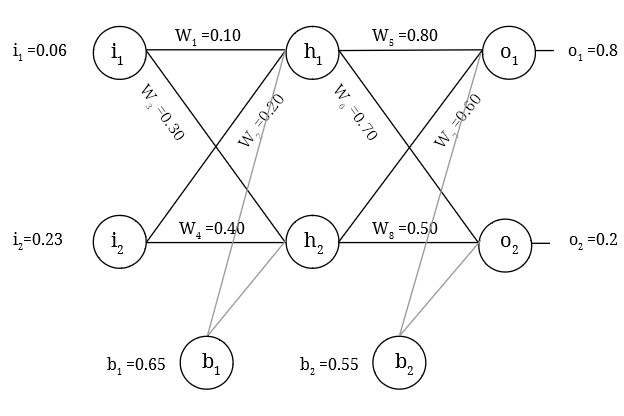
\includegraphics[width=8cm,height=6cm, keepaspectratio]{pics/BackpropExample.jpg}
    \captionsetup{justification=justified,margin=1cm}
    \caption{Basic structure of a neural network with weights and bais initialized}
    \label{fig:bakprop}
\end{figure}

The goal of backpropagation is the adjust the weights such that the neural network can correctly map the input to the output. To begin with consider the neural network in the \ref{fig:bakprop} with inputs to the neural network be $i_{1} = 0.06$ and $i_{2} = 0.23$ to which the neural network should output $o_{1}=0.8$ and $o_{2}=0.2$.

In the forward pass, the neural network is feed in the inputs and given the weights and biases in the \ref{fig:bakprop}, it has to predict the output. It has to figure out the output at each hidden layer neuron, i.e $h_{1}$ and $h_{2}$ and squash each output using activation function and do the same at output layer. The activation function in this case is a \textit{logistic function} of which sigmoid activation is a special case.

To calculate the input at $h_{1}$ as $net_{h_{1}}$ we can use \ref{eq:NNformula} as follows,
\begin{align}
    net_{h_{1}} &= W_{1} * i_{1} + W_{2} * i_{2} +b_{1}\\
    net_{h_{1}} &= 0.10 * 0.60 + 0.20 * 0.23 + 0.65 \\
    net_{h_{1}} &= 0.756 \label{eq:endH1}
\end{align}

And to get the output $out_{h_{1}}$ at $h_{1}$ we apply logistic function to \ref{eq:endH1},
\begin{align}
    out_{h_{1}} &= \frac{1}{1+e^{-net_{h_{1}}}}\\
    out_{h_{1}} &=  \frac{1}{1+e^{0.756}}\\
    out_{h_{1}} &= 0.680 \label{eq:outH1}
\end{align}

Similarly calculating $out_{h_{2}}$ at $h_{2}$ will be:
\begin{align}
    out_{h_{2}} &= 0.681
\end{align}

We can apply same process to output layer neuron, using the output from the hidden layer neuron $h_{1}$ and $h_{1}$ as input.
\begin{align}
    net_{o_{1}} &= W_{5} * h_{1} + W_{7} * h_{2} +b_{2} \label{eq:net_out_1}\\
    net_{o_{1}} &= 0.8 *0.680 +0.6 *0.681 +0.55 \\
    net_{o_{1}} &= 1.50 \label{eq:endO1}
\end{align}
And output $out_{o_{1}}$ at $o_{1}$ we apply logistic function to \ref{eq:endO1}
\begin{align}
    out_{o_{1}} &= \frac{1}{1+e^{-net_{o_{1}}}}\\
    out_{o_{1}} &=  \frac{1}{1+e^{1.50}}\\
    out_{o_{1}} &= 0.8175
\end{align}

Similarly output at $o_{2}$ can be obtained using the same process:
\begin{align}
    out_{o_{2}} &= 0.7957
\end{align}

We have got the output of the final layer, now we can calculate the error. An error function calculates the difference between desired output also known as target and the output predicted by the network. For the purpose of this example we will consider the standard Euclidean distance between the target and the output predicted by the network which we will henceforth refer to as output. 
\begin{align}\label{eq:error}
E_{(target, output)} = \frac{1}{2} (target - output)^{2}    
\end{align}

As we already know the values of the desired output and the predicted output, putting those values in the \ref{eq:error} we can calculate error for $o_{1}$ and $o_{2}$ as follows,

\begin{align}
    E_{o_{1}} &= \frac{1}{2} (0.8-0.8175)^{2}\\
    E_{o_{1}} &= 0.00015  \label{eq:eO1}
\end{align}

Similarly for $E_{o_{2}}$,
\begin{align}\label{eq:eO2}
    E_{o_{2}} &= 0.1774
\end{align}

Combining \ref{eq:eO1} and \ref{eq:eO2} we can calculate total error $E_{total}$ as,
\begin{align}
    E_{total} &= E_{o_{1}} + E_{o_{2}} \label{eq:Etotal}\\
    E_{total} &= 0.17755
\end{align}

Now as the error is calculated we can update the weights so that the predicted outputs are closer to the desired outputs.
Considering the weight $W_{5}$, we want to find out how much change in $W_{5}$ affects the error, i.e the rate of $E_{total}$ w.r.t $W_{5}$, i.e $\frac{\partial E_{total} }{\partial W_{5}}$. 

Applying chain rule, 
\begin{align}
    \frac{\partial E_{total} }{\partial W_{5}} = \frac{\partial E_{total} }{\partial out_{h_{1}}} * \frac{\partial out_{h_{1}} }{\partial net_{h_{1}}} *  \frac{\partial net_{h_{1}} }{\partial W_{5}} \label{eq:backpropMain}
\end{align}

Calculating each term individually,
\begin{align}
    \frac{\partial E_{total} }{\partial out_{h_{1}}} &= \text{change in total loss w.r.t output of $h_{1}$}
\end{align}
From \ref{eq:Etotal}, we can write,
\begin{align}
    E_{total} &= \frac{1}{2}(target_{o_{1}} - out_{o_{1}})^{2} + \frac{1}{2}(target_{o_{2}} - out_{o{1}})^{2}
\end{align}

Taking the partial derivative of $E_{total}$ with respect to $out_{h_{1}}$, the part $\frac{1}{2}(target_{o_{2}} - out_{o{1}})^{2}$ becomes 0 because $out_{h_{1}}$ does not effect it and hence it is a constant.
\begin{align}
    \frac{\partial E_{total}}{\partial out_{o_{1}}} &= 2 * \frac{1}{2}(target_{o_{1}} - out_{o_{1}})^{2 - 1} * -1 + 0\\
    \frac{\partial E_{total}}{\partial out_{o_{1}}} &= -(target_{o_{1}} - out_{o_{1}}) = -(0.8 - 0.8175) = -0.0175 \label{eq:Backprop_2}
\end{align}

Now for the second term in the equation \ref{eq:backpropMain}, we find out the rate of change of $out_{h_{1}}$ w.r.t $net_{h_{1}}$, hence we need to calculate the partial derivative of the logistic function. 
\begin{align}
    out_{h_{1}} &= \frac{1}{1-e^{net_{h_{1}}}}\\
    \frac{\partial out_{h_{1}}}{\partial net_{h_{1}}} &=  out_{h_{1}}*(1-out_{h_{1}}) \\
    \frac{\partial out_{h_{1}}}{\partial net_{h_{1}}} &= 0.8175(1-0.8175) = 0.1491 \label{eq:Backprop_3}
\end{align}
Finally, how much the $n_{o_{1}}$ changes w.r.t $W_{5}$,
\begin{align}
    net_{o_{1}} &= W_{5} * out_{h_{1}} + W_{7} * out_{h_{2}} + b_{2}   \\
    \frac{\partial net_{o_{1}}}{\partial W_{5}} &=  1 * out_{h_{1}} * W_{5}^{(1 - 1)} + 0 + 0 = out_{h_{1}} = 0.680 \label{eq:Backprop_4}
\end{align}

Puttinng \ref{eq:Backprop_2}, \ref{eq:Backprop_3} and \ref{eq:Backprop_4} together, we get:

\begin{align}
    \frac{\partial E_{total} }{\partial W_{5}} &= -0.0175 * 0.1491 * 0.680 = -0.00177429 \label{eq:backprop_6}
\end{align}

To get the new updated weights, we then subtract this the value obtained in \ref{eq:backprop_6} from the old weight multiplying it with learning rate which is 0.1 in our case:

\begin{align}
    W_{5_{new}} = w_5 - \text{learning rate}* \frac{\partial E_{total}}{\partial w_{5}} = 0.8 - 0.1 * (-0.00177429)= 0.800177429
\end{align}

Similarly, we can calculate all the weight updates for $W_{1_{new}}$, $W_{2_{new}}$, $W_{3_{new}}$,$W_{4_{new}}$,\\$W_{6_{new}}$,$W_{7_{new}}$,$W_{8_{new}}$ using the method mentioned above.

\clearpage

\section{Calculating Micro-average Precision Recall and F1-Score}\label{MicroMacroCalculation}
% Please add the following required packages to your document preamble:
% \usepackage{multirow}
% Please add the following required packages to your document preamble:
% \usepackage{multirow}
% Please add the following required packages to your document preamble:
% \usepackage{multirow}

The \ref{tab:precisionRecallF1Score} and \ref{table:Confmatrix1} shows the precision, recall and f1-scores of \gls{BiLSTM} for cluster 1 trained on clustered data show in \ref{fig:question1EvalMacro} and \ref{fig:question1EvalMicro} as BiLSTM-D-ED-C evaluated on document level.

\begin{table}[!ht]
\centering
\begin{tabular}{ccccc}
\textbf{Classes} & \textbf{Precision} & \textbf{Recall} & \textbf{F1-Score} & \textbf{\# Samples} \\ \hline
Agriculture & 0.90 & 0.86 & 0.88 & 50 \\
Audiovisual and Media & 1.00 & 0.10 & 0.18 & 10 \\
Competition & 0.96 & 0.83 & 0.89 & 30 \\
Consumers & 0.59 & 0.65 & 0.62 & 74 \\
Employment and Social Policy & 0.71 & 0.88 & 0.79 & 94 \\
Energy & 0.97 & 0.64 & 0.77 & 56 \\
Enterprise & 0.65 & 0.42 & 0.51 & 26 \\
Environment & 0.70 & 0.84 & 0.76 & 88 \\
Food Safety & 0.93 & 0.82 & 0.87 & 76 \\
Information Society & 0.71 & 0.84 & 0.77 & 80 \\
Internal Market & 0.72 & 0.75 & 0.74 & 148 \\
Public Health & 0.86 & 0.43 & 0.58 & 44 \\
Taxation & 0.95 & 0.71 & 0.82 & 28 \\
Transport & 0.76 & 0.86 & 0.81 & 94 \\ \hline
\textbf{micro avg} & \textbf{0.76} & \textbf{0.76} & \textbf{0.76} & \textbf{898} \\
\textbf{macro avg }& \textbf{0.81} & \textbf{0.69} & \textbf{0.71} & \textbf{898} \\ \hline
\end{tabular}
\captionsetup{justification=centering,margin=1cm}
\caption{CLass-wise precision, recall and f1-score}
\label{tab:precisionRecallF1Score}
\end{table}



\begin{table}[!ht]
\centering
\begin{tabular}{lccccccccccccccccl}
 & \multicolumn{16}{c}{Predicted Values} &  \\
\multicolumn{1}{c}{} &  & \textbf{1} & \textbf{2} & \textbf{3} & \textbf{4} & \textbf{5} & \textbf{6} & \textbf{7} & \textbf{8} & \textbf{9} & \textbf{10} & \textbf{11} & \textbf{12} & \textbf{13} & \textbf{14} & \textbf{} &  \\ \cline{3-16}

\multirow{14}{*}{\rotatebox[origin=c]{90}{Actual Value}} 

& \multicolumn{1}{c|}{\textbf{1}} & \multicolumn{1}{c|}{\hlc[petrol]{43}} & \multicolumn{1}{c|}{0} & \multicolumn{1}{c|}{0} & \multicolumn{1}{c|}{\hlc[yellow]{1}} & \multicolumn{1}{c|}{\hlc[yellow]{2}} & \multicolumn{1}{c|}{0} & \multicolumn{1}{c|}{0} & \multicolumn{1}{c|}{\hlc[yellow]{2}} & \multicolumn{1}{c|}{\hlc[yellow]{2}} & \multicolumn{1}{c|}{0} & \multicolumn{1}{c|}{0} & \multicolumn{1}{c|}{0} & \multicolumn{1}{c|}{0} & \multicolumn{1}{c|}{0} & 50 & \multirow{14}{*}{\rotatebox[origin=c]{270}{Total Samples}} \\ \cline{3-16}

 & \multicolumn{1}{c|}{\textbf{2}} & \multicolumn{1}{c|}{0} & \multicolumn{1}{c|}{1} & \multicolumn{1}{c|}{1} & \multicolumn{1}{c|}{0} & \multicolumn{1}{c|}{0} & \multicolumn{1}{c|}{0} & \multicolumn{1}{c|}{0} & \multicolumn{1}{c|}{0} & \multicolumn{1}{c|}{0} & \multicolumn{1}{c|}{8} & \multicolumn{1}{c|}{0} & \multicolumn{1}{c|}{0} & \multicolumn{1}{c|}{0} & \multicolumn{1}{c|}{0} & 10 &  \\ \cline{3-16}
 
 & \multicolumn{1}{c|}{\textbf{3}} & \multicolumn{1}{c|}{0} & \multicolumn{1}{c|}{0} & \multicolumn{1}{c|}{25} & \multicolumn{1}{c|}{0} & \multicolumn{1}{c|}{0} & \multicolumn{1}{c|}{0} & \multicolumn{1}{c|}{0} & \multicolumn{1}{c|}{0} & \multicolumn{1}{c|}{0} & \multicolumn{1}{c|}{0} & \multicolumn{1}{c|}{1} & \multicolumn{1}{c|}{0} & \multicolumn{1}{c|}{0} & \multicolumn{1}{c|}{4} & 30 &  \\ \cline{3-16}
 
 & \multicolumn{1}{c|}{\textbf{4}} & \multicolumn{1}{c|}{\hlc[red]{2}} & \multicolumn{1}{c|}{0} & \multicolumn{1}{c|}{0} & \multicolumn{1}{c|}{48} & \multicolumn{1}{c|}{1} & \multicolumn{1}{c|}{0} & \multicolumn{1}{c|}{0} & \multicolumn{1}{c|}{2} & \multicolumn{1}{c|}{2} & \multicolumn{1}{c|}{2} & \multicolumn{1}{c|}{11} & \multicolumn{1}{c|}{0} & \multicolumn{1}{c|}{0} & \multicolumn{1}{c|}{6} & 74 &  \\ \cline{3-16}
 
 & \multicolumn{1}{c|}{\textbf{5}} & \multicolumn{1}{c|}{0} & \multicolumn{1}{c|}{0} & \multicolumn{1}{c|}{0} & \multicolumn{1}{c|}{0} & \multicolumn{1}{c|}{83} & \multicolumn{1}{c|}{0} & \multicolumn{1}{c|}{1} & \multicolumn{1}{c|}{0} & \multicolumn{1}{c|}{0} & \multicolumn{1}{c|}{3} & \multicolumn{1}{c|}{7} & \multicolumn{1}{c|}{0} & \multicolumn{1}{c|}{0} & \multicolumn{1}{c|}{0} & 94 &  \\ \cline{3-16}
 
 & \multicolumn{1}{c|}{\textbf{6}} & \multicolumn{1}{c|}{0} & \multicolumn{1}{c|}{0} & \multicolumn{1}{c|}{0} & \multicolumn{1}{c|}{1} & \multicolumn{1}{c|}{0} & \multicolumn{1}{c|}{36} & \multicolumn{1}{c|}{0} & \multicolumn{1}{c|}{14} & \multicolumn{1}{c|}{0} & \multicolumn{1}{c|}{1} & \multicolumn{1}{c|}{2} & \multicolumn{1}{c|}{2} & \multicolumn{1}{c|}{0} & \multicolumn{1}{c|}{0} & 56 &  \\ \cline{3-16}
 
 & \multicolumn{1}{c|}{\textbf{7}} & \multicolumn{1}{c|}{\hlc[red]{3}} & \multicolumn{1}{c|}{0} & \multicolumn{1}{c|}{0} & \multicolumn{1}{c|}{0} & \multicolumn{1}{c|}{3} & \multicolumn{1}{c|}{0} & \multicolumn{1}{c|}{11} & \multicolumn{1}{c|}{2} & \multicolumn{1}{c|}{0} & \multicolumn{1}{c|}{3} & \multicolumn{1}{c|}{4} & \multicolumn{1}{c|}{0} & \multicolumn{1}{c|}{0} & \multicolumn{1}{c|}{0} & 26 &  \\ \cline{3-16}
 
 & \multicolumn{1}{c|}{\textbf{8}} & \multicolumn{1}{c|}{0} & \multicolumn{1}{c|}{0} & \multicolumn{1}{c|}{0} & \multicolumn{1}{c|}{6} & \multicolumn{1}{c|}{2} & \multicolumn{1}{c|}{0} & \multicolumn{1}{c|}{0} & \multicolumn{1}{c|}{74} & \multicolumn{1}{c|}{0} & \multicolumn{1}{c|}{0} & \multicolumn{1}{c|}{2} & \multicolumn{1}{c|}{0} & \multicolumn{1}{c|}{0} & \multicolumn{1}{c|}{4} & 88 &  \\ \cline{3-16}
 & \multicolumn{1}{c|}{\textbf{9}} & \multicolumn{1}{c|}{0} & \multicolumn{1}{c|}{0} & \multicolumn{1}{c|}{0} & \multicolumn{1}{c|}{6} & \multicolumn{1}{c|}{0} & \multicolumn{1}{c|}{0} & \multicolumn{1}{c|}{0} & \multicolumn{1}{c|}{4} & \multicolumn{1}{c|}{62} & \multicolumn{1}{c|}{0} & \multicolumn{1}{c|}{4} & \multicolumn{1}{c|}{0} & \multicolumn{1}{c|}{0} & \multicolumn{1}{c|}{0} & 76 &  \\ \cline{3-16}
 & \multicolumn{1}{c|}{\textbf{10}} & \multicolumn{1}{c|}{0} & \multicolumn{1}{c|}{0} & \multicolumn{1}{c|}{0} & \multicolumn{1}{c|}{0} & \multicolumn{1}{c|}{2} & \multicolumn{1}{c|}{0} & \multicolumn{1}{c|}{0} & \multicolumn{1}{c|}{0} & \multicolumn{1}{c|}{0} & \multicolumn{1}{c|}{67} & \multicolumn{1}{c|}{7} & \multicolumn{1}{c|}{0} & \multicolumn{1}{c|}{0} & \multicolumn{1}{c|}{4} & 80 &  \\ \cline{3-16}
 & \multicolumn{1}{c|}{\textbf{11}} & \multicolumn{1}{c|}{0} & \multicolumn{1}{c|}{0} & \multicolumn{1}{c|}{0} & \multicolumn{1}{c|}{12} & \multicolumn{1}{c|}{7} & \multicolumn{1}{c|}{1} & \multicolumn{1}{c|}{4} & \multicolumn{1}{c|}{1} & \multicolumn{1}{c|}{0} & \multicolumn{1}{c|}{4} & \multicolumn{1}{c|}{111} & \multicolumn{1}{c|}{1} & \multicolumn{1}{c|}{1} & \multicolumn{1}{c|}{6} & 148 &  \\ \cline{3-16}
 & \multicolumn{1}{c|}{\textbf{12}} & \multicolumn{1}{c|}{0} & \multicolumn{1}{c|}{0} & \multicolumn{1}{c|}{0} & \multicolumn{1}{c|}{7} & \multicolumn{1}{c|}{15} & \multicolumn{1}{c|}{0} & \multicolumn{1}{c|}{0} & \multicolumn{1}{c|}{0} & \multicolumn{1}{c|}{1} & \multicolumn{1}{c|}{0} & \multicolumn{1}{c|}{2} & \multicolumn{1}{c|}{19} & \multicolumn{1}{c|}{0} & \multicolumn{1}{c|}{0} & 44 &  \\ \cline{3-16}
 & \multicolumn{1}{c|}{\textbf{13}} & \multicolumn{1}{c|}{0} & \multicolumn{1}{c|}{0} & \multicolumn{1}{c|}{0} & \multicolumn{1}{c|}{0} & \multicolumn{1}{c|}{2} & \multicolumn{1}{c|}{0} & \multicolumn{1}{c|}{0} & \multicolumn{1}{c|}{1} & \multicolumn{1}{c|}{0} & \multicolumn{1}{c|}{2} & \multicolumn{1}{c|}{1} & \multicolumn{1}{c|}{0} & \multicolumn{1}{c|}{20} & \multicolumn{1}{c|}{2} & 28 &  \\ \cline{3-16}
 & \multicolumn{1}{c|}{\textbf{14}} & \multicolumn{1}{c|}{0} & \multicolumn{1}{c|}{0} & \multicolumn{1}{c|}{0} & \multicolumn{1}{c|}{0} & \multicolumn{1}{c|}{0} & \multicolumn{1}{c|}{0} & \multicolumn{1}{c|}{1} & \multicolumn{1}{c|}{6} & \multicolumn{1}{c|}{0} & \multicolumn{1}{c|}{4} & \multicolumn{1}{c|}{2} & \multicolumn{1}{c|}{0} & \multicolumn{1}{c|}{0} & \multicolumn{1}{c|}{81} & 94 &  \\ \cline{3-16}
\end{tabular}
\captionsetup{justification=centering,margin=1cm}
\caption{Confusion matrix for cluster 1 of \gls{BiLSTM} trained on English and German corpus}
\label{table:Confmatrix1}
\end{table}


To calculate the micro average precision we first need the values of \gls{TP} and \gls{FP}. These values are available in confusion matrix in \ref{table:Confmatrix1}

As descibed in \ref{backgroundEvaluationMatrices}, we calculate micro-average precision for a classifier by adding values of $\frac{TP}{TP+FP}$ for all the classes.

Hence, for \textit{Agriculture} the value in the \ref{table:Confmatrix1} for \gls{TP} is highlighted in \hlc[petrol]{blue} and \gls{FP} are highlighted in \hlc[red]{red} and \gls{FN} are highlighted in \hlc[yellow]{yellow}.

 \begin{align}
    \text{Micro-Avg Precision for \textit{Agriculture}} = \frac{43}{43+2+3} 
\end{align}

 \begin{align}
    \text{Micro-Avg Recall for \textit{Agriculture}} = \frac{43}{43+1+2+2+2} 
\end{align}
 
 
Similarly, getting the values of all the classes from the \ref{table:Confmatrix1} we get,

\begin{align*}
    \text{Micro-Avg Precision} =& \frac{43+1+25+48+83}{43+2+3+1+0+25+1+48+33+83+34} \\
    & + \frac{36+11+74+62+67+111}{11+6+74+32+62+5+67+27+111+43}\\
    & + \frac{19+20+81}{19+3+20+1+81+26}
\end{align*}

\begin{align}
    \text{Micro-Avg Precision} = \frac{618}{898} = 0.7583 \approx 0.76
\end{align}

Similarly, to calculate the micro-average recall we get all the \gls{TP} and \gls{TN} values from the confusion matrix,
\begin{align*}
    \text{Micro-Avg Precision} =& \frac{43+1+25}{43+1+2+2+2+8+1+1+25+1+4} \\
    & + \frac{48+83}{48+2+1+2+2+2+11+6+83+1+3+7}\\
    & + \frac{36+11}{36+1+14+1+2+2+11+3+3+2+3+4}\\
    & + \frac{74+62+67}{74+6+2+2+4+62+6+4+4+67+2+7+4}\\
    & + \frac{111}{111+12+7+1+4+1+4+1+1+6}\\
    & + \frac{19+20}{19+7+15+1+2+20+2+1+2+1+2}\\
    & + \frac{81}{81+1+6+4+2}
\end{align*}

\begin{align}
    \text{Micro-Avg Recall} = \frac{618}{898} = 0.7583 \approx 0.76
\end{align}


\begin{align}
    \text{Micro-Avg F1-Score} = &2 * \left ( \frac{\text{micro-avg precision} * \text{micro-avg recall}}{\text{micro-avg precision}+\text{micro-avg recall}} \right ) \\
                              = &2 * \left ( \frac{0.76*0.76}{0.76+0.76} \right ) \\
                              = & 0.76  
\end{align}


To, calculate macro average precision, we need to add the per-class precision values from \ref{tab:precisionRecallF1Score}

Macro-avg precision is, 
\begin{align*}
    =\frac{\text{\small 0.90+1.00+0.96+0.59+0.71+0.97+0.65+0.70+0.93+0.71+0.72+0.86+0.95+0.76}}{\text{\small 14}}
\end{align*}
\begin{align}
    \text{Macro-Avg Precision} =  \frac{11.41}{14} \approx 0.81
\end{align}

Macro-avg recall is, 
\begin{align*}
    =\frac{\text{\small 0.86+0.10+0.83+0.65+0.88+0.64+0.42+0.84+0.82+0.84+0.75+0.43+0.71+0.86}}{\text{\small 14}}
\end{align*}
\begin{align}
    \text{Macro-Avg Precision} =  \frac{}{14} = 0.68785714 \approx 0.69
\end{align}


\section{Visualization of word embeddings} \label{visualEmb}

The visualization of the ten randomly selected words \textit{industrie, alike, customary, siting, thailand, multidisciplinarity, sites, transaktions, hauskatze, formetanate} is given below.

The first step in visualization is to reduce the dimension, for this we are using t-Distributed Stochastic Neighbor Embedding (t-SNE) dimensionality reduction technique. Reducing the dimension is necessary because these words are in 300 dimensional vector space and it would be impossible to consider all the dimension during visualization.

\begin{figure}[!ht]
    \centering
    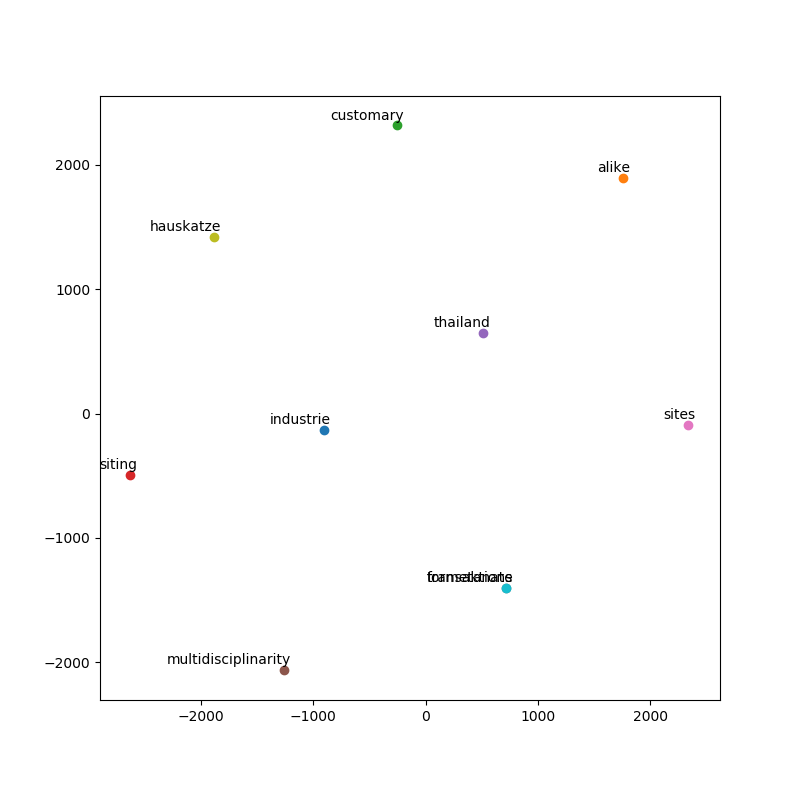
\includegraphics[width=10cm,height=10cm,keepaspectratio]{pics/before_selected_embedding.png}
    \captionsetup{justification=centering,margin=1cm}
    \caption{Visualization of ten randomly selected words for frozen word embedding}
    \label{fig:frozenAppendix}
\end{figure}

As it is clear from the \ref{fig:frozenAppendix} that words like \textit{transaktions} and \textit{formetanate} are not present in the general-purpose embedding and hence their embedding weights are zero and they are coinciding with one another in the \ref{fig:frozenAppendix}.

\begin{figure}[!ht]
    \centering
    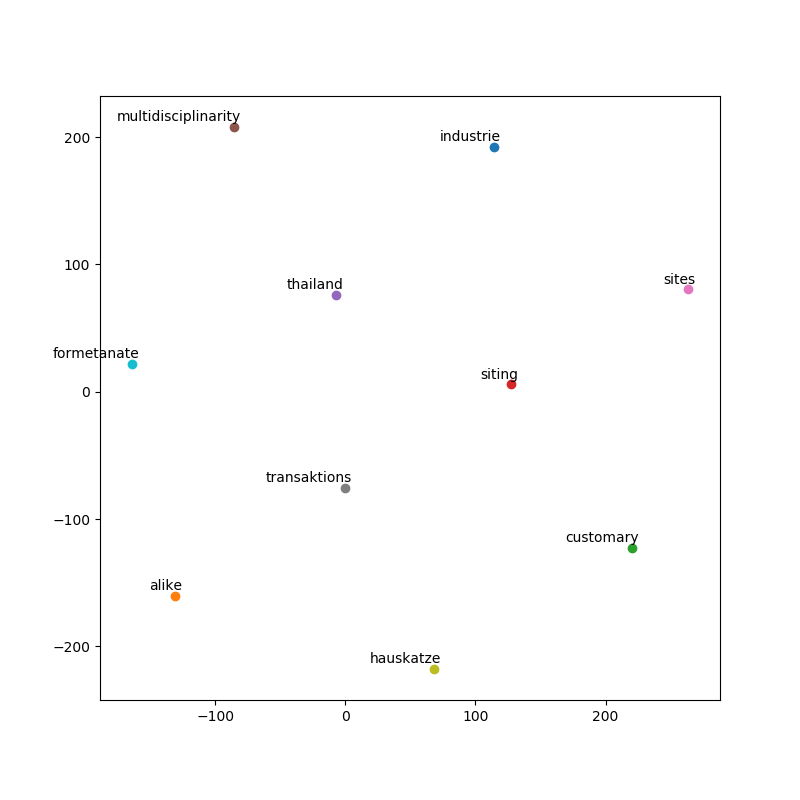
\includegraphics[width=10cm,height=10cm,keepaspectratio]{pics/after_selected_embedding.png}
    \captionsetup{justification=centering,margin=1cm}
    \caption{Visualization of ten randomly selected words for trained word embedding}
    \label{fig:trainedAppendix}
\end{figure}

So we can see that after training \textit{transaktions} and \textit{formetanate} now are at different position \ref{fig:trainedAppendix}. To see the effect of training on these words, we added two new words (\textit{katze},\textit{normal}) and visualized it.

\begin{figure}[!ht]
    \centering
    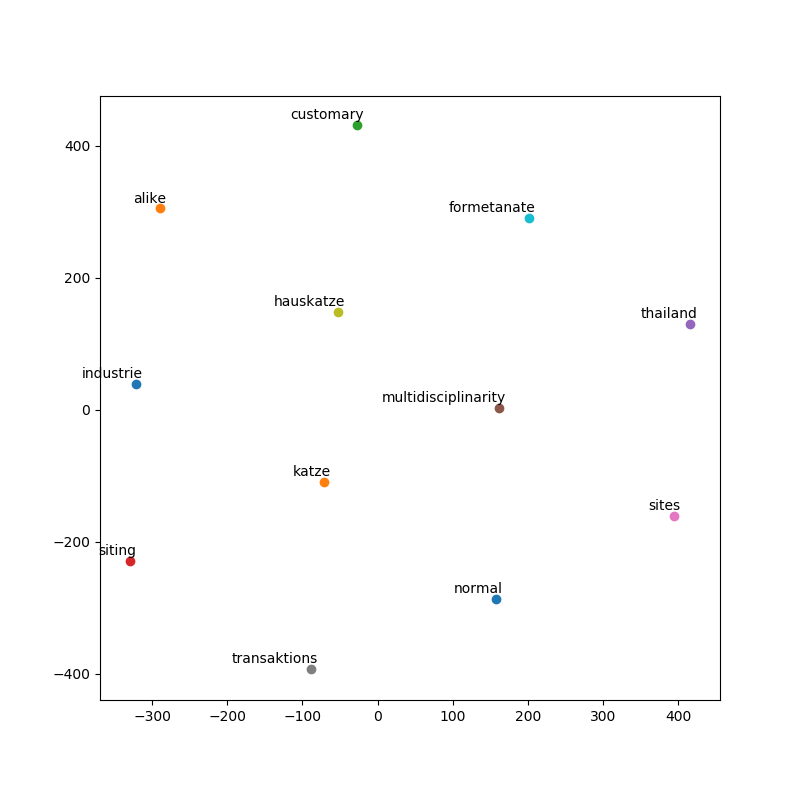
\includegraphics[width=10cm,height=10cm,keepaspectratio]{pics/before_selected_added_embedding.png}
    \captionsetup{justification=centering,margin=1cm}
    \caption{Visualization after adding word \textit{katze} and \textit{normal} to the frozen embeddings}
    \label{fig:frozenAppendixAdded}
\end{figure}

\begin{figure}[!ht]
    \centering
    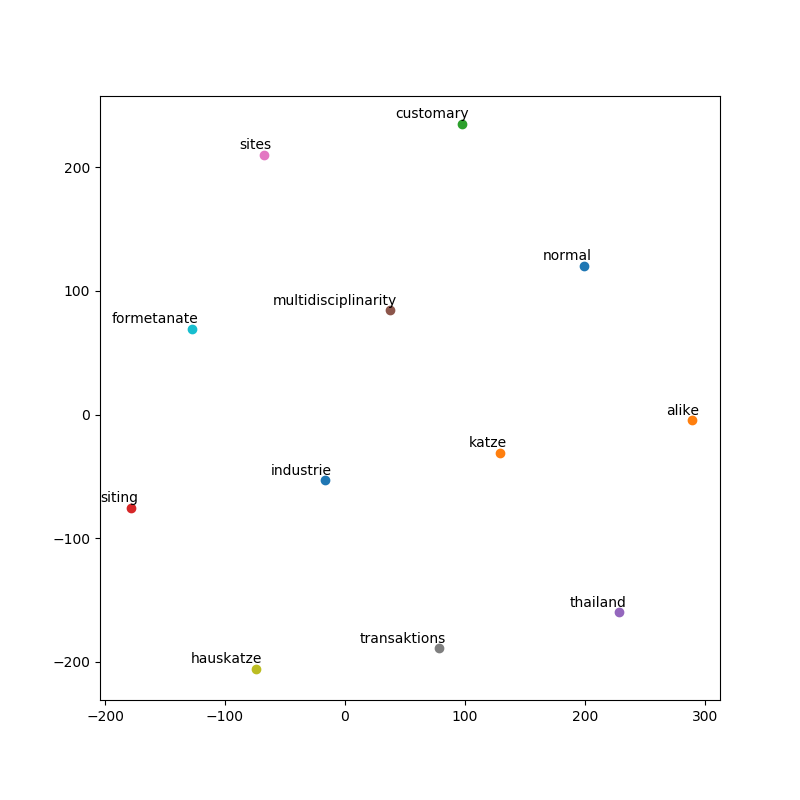
\includegraphics[width=10cm,height=10cm,keepaspectratio]{pics/after_selected_added_embedding.png}
    \captionsetup{justification=centering,margin=1cm}
    \caption{Visualization after adding word \textit{katze} and \textit{normal} to the trained embeddings}
    \label{fig:trainedAppendixAdded}
\end{figure}

\clearpage
The figure \ref{fig:frozenAppendixAdded} shows the added two words before the training of the word embeddings, as we can see that the word \textit{katze} and \textit{hauskatze} are not that far from each other. We can calculate the cosine similarity between these two words before training as follows 
\begin{align}
    \text{cosine similarity before training}_{(katze, hauskatze)} &= \frac{\textbf{katze} \cdot \textbf{hauskatze}}{\left \| \textbf{katze}\right \| \left \| \textbf{hausekatze} \right \|}\\\\
    &= 0.78172445
\end{align}

and the cosine similarity after the embedding is trained is as follows,

\begin{align}
    \text{cosine similarity after training}_{(katze, hauskatze)} = 0.8065112
\end{align}

Similarly, for the words \textit{customary} and \textit{normal} which are synonyms, the cosine similarity before training the embedding and after training embedding 

\begin{align}
    \text{cosine similarity before training}_{(customary, normal)} = 0.18904422
\end{align}

\begin{align}
    \text{cosine similarity after training}_{(katze, hauskatze)} = 0.28809269
\end{align}



Hence, training the embedding further is necessary.
\ifgerman{\chapter*{Erklärung}}{\chapter*{Statement of Authorship / Selbstständigkeitserklärung}}


% ATTENTION: Here are some manual word breaks.

Hiermit erkläre ich, dass ich die vorliegende Masterarbeit selbstständig und außschließlich unter Verwendung der angegebenen Literatur und Hilfsmittel angefertigt habe.\\
Die aus fremden Quellen direkt oder indirekt übernommenen Stellen sind als solche kenn-tlich gemacht.\\

Die Arbeit wurde bisher in gleicher oder ähnlicher Form weder einer anderen Prüfungsbehörde vorgelegt oder noch anderweitig veröffentlicht.
\vspace{100pt}

\doublesignature{Unterschrift}{Datum}

\newpage
%*********************************************************************%
% LITERATURE                                                          %
%*********************************************************************%

\cleardoublepage
\phantomsection
\addcontentsline{toc}{chapter}{\bibname} % 
\bibliographystyle{alpha} % plain gerplain abbrvnat unsrtnat alphag alpha
% in a thesis you have space... use full names
\bibliography{literature/IEEEfull,literature/MYfull,literature/literature}
% in a paper, space is limited. use abreviations
%\bibliography{../literature/IEEEabrv,../literature/MYabrv,../literature/literature}

%*********************************************************************%
% ERKLÄRUNG                                                           %
%*********************************************************************%

\ifnotdraft{
	\cleardoublepage
	\phantomsection
	\printindex
	\thispagestyle{empty}
\vspace*{38\baselineskip}
\hbox to \textwidth{\hrulefill}
\par
Hiermit erkl\"are ich, dass ich die vorliegende Arbeit selbst\"andig verfasst und
keine anderen als die angegebenen Quellen und Hilfsmittel verwendet habe.

\signatureplace, den \signaturedate

%%%%%%%%%%%%%%%%%%%%%%%%%%%%%%%%%%%%%%%%%%%%%%%%%%%%%%%%%%%%%%%%%%%%%%%%
%% Hinweis:
%%
%% Diese Erklärung wird von der Prüfungsordnung für Diplomarbeiten 
%% verlangt und ist zu unterschreiben. Für Studienarbeiten ist diese
%% Erklärung nicht zwingend notwendig, schadet aber auch nicht.
%%%%%%%%%%%%%%%%%%%%%%%%%%%%%%%%%%%%%%%%%%%%%%%%%%%%%%%%%%%%%%%%%%%%%%%%
\clearpage

}

\end{document}